% Package obligatoire : type de document
\documentclass[a4paper,12pt,twoside]{book}

% Encodage
\usepackage{fontspec}

% Annexes (à déclarer avant hyperref)
\usepackage{appendix}

% Le package hyperref avec des options, si en local
\usepackage[pdfusetitle, pdfsubject ={Mémoire TNAH}, pdfkeywords={les mots-clés}]{hyperref}

% Langues
\usepackage[english,french]{babel}
% Commande personnalisée pour la typographie des langues
\newcommand{\langue}[1]{\emph{#1}}

% Configurer le document selon les normes de l'école
\usepackage[margin=2.5cm]{geometry} % marges
\usepackage{setspace} % espacement qui permet ensuite de définir un interligne
\onehalfspacing % interligne de 1.5
\setlength\parindent{1cm} % indentation des paragraphes à 1 cm

% Table des matières
\addto\captionsfrench{
\renewcommand*\contentsname{Contenu de la documentation}
}
\usepackage[nottoc]{tocbibind}% Pour ajouter la biblio à la TDM sans numérotation de chapitre

% Bibliographie
\usepackage[backend=biber, sorting=nyt, style=enc, maxbibnames=10]{biblatex}
\addbibresource{./biblio.bib}
\defbibnote{sources-cds}{Cette liste contient les cotes de l'inventaire numérique de la correspondance, \cite{KorrespondenzConstanceSalm2022}~:}

%\nocite{*}

% Sigles et acronymes
\usepackage[automake,acronym,toc]{glossaries}
\makeglossaries
% Acronymes
\newacronym{alto}{ALTO}{\textit{Analyzed Layout and Text Object} (format XML pour la description des textes et de leur mise en page)}
\newacronym{atilf}{ATILF}{Analyse et Traitement Informatique de la Langue Française (Centre National de la Recherche Scientifique-Universié de Lorraine)}
\newacronym{bnf}{BnF}{Bibliothèque nationale de France}
\newacronym{cds}{C.~de Salm}{Constance de Salm}
\newacronym{cg2c2v}{Corr.~g., 2e copie, 2e vol.}{long}
\newacronym{cremma}{Cremma}{Consortium Reconnaissance d’Écriture Manuscrite des Matériaux Anciens}
\newacronym{dahn}{DAHN}{Dispositif de soutien à l’Archivistique et aux Humanités Numériques (partenariat entre l’Inria, l’Université du Mans et l’EHESS)}
\newacronym{dhi}{DHIP}{Deutsches Historisches Institut, Paris}
\newacronym{enc}{ENC}{École nationale des chartes}
\newacronym{fud}{FuD}{Die Virtuelle Forschungsumgebung für die Geistes- und Sozialwissenschften (système de gestion de bases de données, Trèves)}
\newacronym{galcor}{Gallic(orpor)a}{Gallic(orpor)a (projet financé par Huma-Num et le BnF DataLab)}
\newacronym{htr}{HTR}{\textit{Handwritten Text Recognition} (reconnaissance automatique d'écriture manuscrite)}
\newacronym{json}{Json}{\textit{JavaScript Object Notation} (format standard de représentation de données structurées)}
\newacronym{lai}{LAI}{Lettre Absente de l'Inventaire en ligne}
\newacronym{lectaurep}{Lectaurep}{Lecture Automatique de Répertoires (initiative conjointe du Minutier central des notaires de Paris des Archives Nationales, de l’Inria et de l’EPHE, en partenariat avec le Ministère de la Culture)}
\newacronym{ocr}{OCR}{\textit{Optical Character Recognition}}
\newacronym{odd}{ODD}{\textit{One Document Does it all} (schéma de validation d'une édition nativement numérique au format \gls{tei})}
\newacronym{segmonto}{SegmOnto}{SegmOnto~: A Controlled Vocabulary to Describe the Layout of Pages}
\newacronym{tei}{TEI}{Text Encoding Initiative}
\newacronym{xml}{XML}{\textit{Extensible Markup Language} (standard du W3C pour l'expression de données en arborescence)}
% Glossaire
\newglossaryentry{prédiction}{name=prédiction,description=Transcription automatique de lignes d'écriture par un algorithme de reconnaissance des caractères.}
\newglossaryentry{segmentation}{name=segmentation,description=Analyse optique d'une image permettant d'obtenir la reconnaissance des régions et des lignes d'écriture.}

% Images
\usepackage{graphicx}

% Citations
\usepackage{csquotes}

% Blocs de code
\usepackage[cache=false]{minted}%  fait disparaître le message d'erreur mais le contenu ne s'affiche plus
%\usepackage{pifont}



% Schéma d'arborescence de dossiers
\usepackage[edges]{forest}
\usepackage{array}
\definecolor{folderbg}{RGB}{124,166,198}
\definecolor{folderborder}{RGB}{110,144,169}
\newlength\Size
\setlength\Size{4pt}
\tikzset{%
	folder/.pic={%
		\filldraw [draw=folderborder, top color=folderbg!50, bottom color=folderbg] (-1.05*\Size,0.2\Size+5pt) rectangle ++(.75*\Size,-0.2\Size-5pt);
		\filldraw [draw=folderborder, top color=folderbg!50, bottom color=folderbg] (-1.15*\Size,-\Size) rectangle (1.15*\Size,\Size);
	},
	file/.pic={%
		\filldraw [draw=folderborder, top color=folderbg!5, bottom color=folderbg!10] (-\Size,.4*\Size+5pt) coordinate (a) |- (\Size,-1.2*\Size) coordinate (b) -- ++(0,1.6*\Size) coordinate (c) -- ++(-5pt,5pt) coordinate (d) -- cycle (d) |- (c) ;
	},
}
\forestset{%
	declare autowrapped toks={pic me}{},
	pic dir tree/.style={%
		for tree={%
			folder,
			font=\itshape,
			grow'=0,
		},
		before typesetting nodes={%
			for tree={%
				edge label+/.option={pic me},
			},
		},
	},
	pic me set/.code n args=2{%
		\forestset{%
			#1/.style={%
				inner xsep=2\Size,
				pic me={pic {#2}},
			}
		}
	},
	pic me set={directory}{folder},
	pic me set={file}{file},
}
\newcommand{\fname}[2]{\begin{tabular}{m{1cm}@{\quad}m{4cm}}#1 & \normalfont#2\end{tabular}}

% Typographie des siècles
\newcommand{\siecle}[1]{\textsc{#1}\ieme}

% DOCUMENT
\begin{document}
	
	\tableofcontents
	
	\chapter*{Présentation}
	\addcontentsline{toc}{chapter}{Présentation}% Ajoute à la table des matières sans numérotation
	
		\section*{Contexte}
			\addcontentsline{toc}{section}{Contexte}
			\gls{cds} (1767-1845), femme de lettres française, a entretenu une vaste correspondance à partir de son mariage avec de nombreux intellectuels en Allemagne, en France, en Russie.
	
			Le projet de publier numériquement sa correspondance est né de l'intérêt pour les relations entre noblesses française et allemande au sein du \gls{dhi}. Il en a résulté la production d'un site \textit{Wordpress} adossé au système de base de données \href{https://fud.uni-trier.de/}{\gls{fud}}. Les notices de plus de 11000 lettres, publiées sur le site \href{https://constance-de-salm.de}{constance-de-salm.de}, associent la reproduction numérique des documents manuscrits (lettres, copies, brouillons, recueils) avec leurs métadonnées descriptives, ainsi qu'une transcription de la première ligne de chaque lettre.
	
		\section*{Objectifs}
			\addcontentsline{toc}{section}{Objectifs}
			L'objectif du stage consiste à mettre en place un flux de production automatisé pour l'édition des lettres au format \gls{tei}. 
			
			On s'appuiera pour cela sur les instruments et la documentation produits dans le cadre du projet \gls{dahn}, fondé sur l'édition de la correspondance de Paul d’Estournelles de Constant (1852-1924)\footcite{chiffoleauDAHNProject}.
			
			Il s'agit en particulier d'identifier les points de difficulté que posent le traitement de ce vaste corpus tant du point de vue de la transcription automatisée des documents que du point de vue de leur encodage au format \gls{tei}. 
			
			Il serait notamment souhaitable, au terme du stage de disposer d'un flux de production pour l'édition d'un volume de recueil de lettres.
				
	\chapter[HTR~: état des lieux]{Reconnaissance automatique des écritures manuscrites \\ \large Un état des lieux}
		
		La reconnaissance automatique des écritures manuscrites (ou \gls{htr}) se fonde sur des principes techniques globalement similaires à la reconnaissance optique des caractères (imprimés) (ou \gls{ocr}), et il est courant de ne pas établir de distinction fondamentale entre ces deux techniques, bien que leur mise en application fasse appel à des logiciels différents (il sera question plus loin de Transkribus et d'eScriptorium)
		\footnote{Certaines publications tentent d'introduire une distinction entre les deux techniques dans la mesure où les techniques d'\gls{ocr} se fondent souvent sur la reconnaissance caractère par caractère et non sur la reconnaissance des lignes (employée par toutes les techniques \gls{htr}), mais ce n'est pas toujours le cas (\cite{stokesEScriptoriumVREManuscript2021}).}.
		
		\section{Principes généraux}
		
			La reconnaissance automatique des écritures manuscrites recouvre quatre phases indissociables et complémentaires~:
			
			\begin{enumerate}
				\item L'import des images dans l'application~: dans le cas présent il s'agit simplement de convertir les images stockées sur un disque dur du format non compressé \textsf{tiff} (qui permet d'archiver des images de la meilleure qualité possible) vers le format compressé \textsf{jpeg} (qui permet de travailler avec une bonne qualité d'image sous la forme de fichiers plus légers)~;
				\item La \gls{segmentation} des pages, au cours de laquelle les textes contenus sur chaque page sont repérés par zone et les lignes qui composent ces zones de texte sont identifiées et numérotées dans l'ordre de lecture (ce sans quoi la transcription produite serait inexploitable~!)~;
				\item La reconnaissance des écritures proprement dite, ou transcription automatique, qui procède à l'identification de chaque caractère sur les lignes précédemment repérées~;
				\item La compilation des lignes transcrites dans un document cohérent pour chaque image traitée et l'export du résultat dans un format exploitable~: on a en l'occurrence retenu le format \gls{alto}, maintenu par la Bibliothèque du Congrès et privilégié par la \gls{bnf}\footcite{TechniquesFormatsConversion2022, stokesEScriptoriumVREManuscript2021}.
			\end{enumerate}
			
			Les phases les plus délicates sont naturellement la troisième et la quatrième en ce qu'elles reposent toutes deux sur l'apprentissage machine (\textit{machine learning}) ou apprentissage supervisé. Cette méthode implique la constitution de données d'entraînement de façon manuelle, données qui sont ensuite analysées de manière statistique par l'outil informatique. Au terme de cette phase est produit un modèle capable, avec un taux d'acuité (ou \textit{accuracy}) exprimé en pourcentage, de reproduire l'opération initialement effectuée manuellement, qu'il s'agisse de la reconnaissance des régions et des lignes d'écriture (\gls{segmentation}) ou de la transcription des caractères.
			
			Ce processus d'entraînement comporte deux phases longues et consommatrices d'énergie~:
			
			\begin{enumerate}
				\item La constitution des données d'entraînement par l'homme~: segmenter et transcrire à la main un nombre de pages suffisamment important pour un entraînement efficace~;
				\item L'entraînement par la machine, qui demande une puissance de calcul très importante (selon le matériel utilisé et la quantité de données, un entraînement peut durer de quelques heures à… quelques semaines) et donc une forte consommation d'électricité.
			\end{enumerate}
			
			Une fois qu'un modèle satisfisant est produit, son utilisation est en revanche rapide et très peu consommatrice~; ainsi, plus la quantité de données pouvant être traitées par un modèle est grande, plus l'opération dans son ensemble est rentable. De plus, un modèle produit à partir de sources déterminées peut être réutilisé dans un contexte différent, et fort heureusement, le développement des projets faisant appel à la reconnaissance automatique des écritures manuscrites a engendré la multiplication des données d'entraînement et des modèles pré-entraînés. Il ne s'agit donc pas de partir de zéro mais d'abord et avant tout d'identifier les meilleurs modèles à partir desquels procéder à de nouveaux entraînements ou affinages, afin de les rendre plus adéquats aux sources sur lesquels on travaille.
			
			Il faut aussitôt mettre un bémol à cet état de faits encourageant~: les deux phases de la \gls{segmentation} et de la transcription ne jouissent pas du tout des mêmes possibilités quant à la réutilisation de modèles. Si les modèles de transcription sont déjà nombreux et, lorsque les écritures ne sont pas trop cursives, peuvent être affinés de façon satisfaisante sur de nouvelles écritures avec seulement une dizaine de page transcrites à la main, il n'en va pas de même des modèles de \gls{segmentation}, comme on aura l'occasion de le voir plus loin
			\footnote{Voir \textit{infra} \ref{lieu-segmentation}, p.~\pageref{lieu-segmentation}.}.
		
		\section{La recherche à l'heure de l'HTR}
		
			Dans le cadre du projet \gls{cremma}-Lab soutenu par le DIM MAP, le centre
			Jean-Mabillon (École nationale des chartes), en partenariat avec le
			LAMOP et le LabEX Hastec, a organisé les 23 et 24 juin 2022 un colloque
			intitulé \textit{Documents anciens et reconnaissance automatique des écritures manuscrites}
			\footnote{Comité d'organisation~: Ariane Pinche et Floriane Chiffoleau. Comité scientifique~: Jean-Baptiste Camps, Alix Chagué, Thibault Clérice, Frédéric Duval, Vincent Jolivet, Benjamin Kiessling, Nicolas Perreaux, Ariane Pinche, Laurent Romary, Peter Stokes. \cite{DocumentsAnciensReconnaissance}}.
			
			Ce colloque a été l'occasion de rassembler une communauté scientifique
			représentant les pays du sud de l'Europe (France, Italie, Grêce,
			Portugal, Suisse) ainsi que quelques équipes nords-américaines autour
			des enjeux, des finalités, des problèmes et des solutions d'avenir de la
			reconnaissance automatique des écritures manuscrites.
			
			Le compte-rendu analytique qui en est donné dans les pages qui suivent constitue un état de l'art des projets et des techniques appliquées à l'HTR.
			
			\subsection{Des finalités et des publics multiples}
		
				Les finalités de l'HTR sont multiples. Elles concernent aussi bien les
				scientifiques qu'un public élargi aux savants et aux curieux des sources
				écrites anciennes. Les projets \textit{Crimes et châtiments}\footcite{paupeCursiveXVIIeSiecle2022} et
				\textit{Lettres en lumières}\footcite{fizaineLettresLumieres2022a} ont démontré l'intérêt de l'HTR pour
				ouvrir la lecture des textes anciens en dehors du monde académique ou
				pour le développement de projets de transcription contributive.
				
				Pour le public scientifique, l'HTR est en mesure de rendre accessibles
				des données selon plusieurs modalités. Le projet POPP (Projet
				d'Océrisation des Recensements de la Population Parisienne) a montré
				comment elle permet de construire de vastes bases de données par
				l'extraction d'informations de recensements historiques\footcite{constumReconnaissanceExtractionInformations2022}. Le projet Sofer
				Mahir a proposé une méthode pour l'établissement d'éditions critiques\footcite{stoklbenezraHTRCriticalEdition2022}, ce qui impose d'ajouter à la
				transcription des documentsune étape de structuration de leur
				hiérarchie, les différents témoins d'un même texte affectant souvent des
				mises en page différentes. Les travaux de thèse de doctorat de
				Christophe Tufféry\footcite{tufferyRetourExperiencesUtilisation2022} ont
				mis en évidence quant à eux un exemple de développement d'application
				visant à proposer, à partir de la transcription de carnets de fouilles
				archéologiques, des visualisations de ces données pour restituer
				l'histoire d'une fouille programmée.
				
				Outre la mise à disposition des sources textuelles ou des données
				qu'elles contiennent, l'HTR offre des possibilités de traitement massif
				de ces données avec plusieurs types d'objectifs. Les
				\textit{Expérimentations pour l'analyse automatique de sources chinoises anciennes}\footcite{bizais-lilligExperimentationsPourAnalyse2022} ont
				montré l'intérêt de l'HTR pour suivre l'utilisation de textes à travers
				les siècles. Dans les domaines épigraphique et paléographique également,
				les algorithmes de reconnaissance d'écriture peuvent servir d'outil à
				l'analyse des mots et des glyphes\footcite{boschettiEpiSearchRecognisingAncient2022}~; l'analyse des erreurs de reconnaissance peut également être exploitée afin dégager des
				caractéristiques d'évolution des écritures\footcite{paraskeviHTRHandwrittenPaleographic2022}.
				
				Enfin le projet CHAMDOC a illustré le fait que l'HTR peut intervenir
				dans la préservation des langues écrites en péril, comme c'est le cas du
				cham ancien, langue véhiculaire utilisée dans des inscriptions gravées
				au Vietnam, du VIe au XVIIe siècle\footcite{schweyerAnalyseReconnaissanceIndexation2022}.
		
			\subsection{eScriptorium et Kraken~: infrastructures et développements}
			
				Le paysage des applications dédiées à l'HTR se partage depuis 2019 entre
				Transkribus (2016) et eScriptorium. Certains projets de recherche ont eu
				l'occasion de tester les deux applications\footcite{leblancTranskribusEScriptoriumRetour2022, paupeCursiveXVIIeSiecle2022} et ainsi fait part de leurs
				expériences. L'entraînement de modèles \gls{htr} est un processus exigeant de
				très grandes capacités de calcul, et donc des infrastructures coûteuses.
				L'infrastructure \gls{cremma} ouvrira bientôt au public des institutions
				académiques partenaires une instance d'eScriptorium\footcite{marguin-hamonDiscoursOuverturePresentation2022} dotée de trois GPU
				(\textit{Graphics Processing Unit} ou unité de traitement graphique),
				chacune représentant en moyenne un coût d'une dizaine de milliers
				d'euros. L'infrastructure FoNDUE de l'université de Genève bénéficie
				quant à elle de la puissance du superordinateur (HPC) de l'université,
				doté de 150 GPU. La recherche des meilleures performances des
				entraînements de modèles consiste généralement à trouver le bon
				équilibre entre temps de calcul par image et nombre de tâches lancées en
				parallèle\footcite{gabayFoNDUELightweightHTR2022}.
				
				Les développements en cours de l'interface eScriptorium donneront lieu
				dans un avenir proche à une fonctionnalité de recherche des termes
				transcrits, à du balisage TEI basique, à la possibilité d'annotation
				graphique des pages, à l'alignement automatique d'un texte existant sur
				une image et à l'intégration de l'ordre des lignes dans l'entraînement
				des modèles de {segmentation}. Quant à l'application Kraken, sur laquelle
				se fonde l'interface eScriptorium, sa dernière version stable (4)
				propose de nouvelles bibliothèques d'entraînement et une meilleure
				accessibilité de son API. Elle affiche en outre une amélioration des
				performances pour les modèles de reconnaissance d'écriture, la
				reconstruction de lacunes et une nouvelle technologie de {segmentation}
				des régions et des lignes d'écriture (\textit{layout analysis})~: grâce à
				l'utilisation de la technologie Transformers, la détection de
				l'orientation des lignes est désormais plus robuste, et il devient
				possible de segmenter des lignes qui se croisent. Cette innovation est
				néanmoins très exigeante sur le plan de l'infrastructure et renchérit le
				coût technologique de l'entraînement de modèles\footcite{kiesslingNewDevelopmentsKraken2022}.
		
		\section{Produire des modèles}
		
			\subsection{Explorer de nouveaux types d'écriture}
			
				Les projets de recherche présentés à l'occasion du colloque s'emploient
				à étendre la zone de compétence des modèles \gls{htr} dans les domaines les
				plus variés. Tandis que les écritures livresques médiévales sont de
				mieux en mieux couvertes du XIe au XVe siècle par les modèles produits
				dans le cadre du projet \gls{cremma}~: Arabica, Bicerin et bientôt Cortado\footcite{campsCremmaLabProjectsTranscription2022}, le projet e-NDP
				s'emploie à travers les sources du chapitre de Notre-Dame de Paris à
				entraîner des modèles pour des écritures nouvelles~: \textit{cursiva},
				\textit{textualis}, prégothique, semihybride\footcite{torresaguilarModelisationAffinageHTR2022}. En effet les écritures
				cursives font actuellement partie des fronts pionniers de l'entraînement
				des modèles, que ce soit pour le Moyen Âge, le XVIIe siècle\footcite{paupeCursiveXVIIeSiecle2022}, ou dans le contexte de projet
				diachroniques comme l'étude des archives inquisitoriales portugaises
				pour la période allant 1536 à 1821\footcite{baudryArchivesInquisitorialesPortugal2022}, ou encore des sources
				très contemporaines comme les carnets de fouilles archéologiques du XXe
				siècle\footcite{tufferyRetourExperiencesUtilisation2022}. Comme l'a montré
				le projet TraPrInq (\textit{Transcribing the court records of the
					Portuguese Inquisition}, 1536-1821), l'entraînement de ces modèles doit
				parfois relever le défi de la variété paléographique, des mélanges de
				langues et de types d'écriture (latine, arabe, hébraïque)~; de la
				variété aussi des types de documents dont découle des mises en pages
				hétérogènes, de la variété des supports également, susceptible
				d'infléchir l'efficacité des entraînements\footcite{baudryArchivesInquisitorialesPortugal2022}. D'autre projets
				tentent de couvrir une diachronie encore plus longue, comme la création
				d'un corpus de fictions littéraires allant du XIe siècle à nos jours\footcite{campsCremmaLabProjectsTranscription2022}. Enfin, les projets HTR
				s'étendent également en direction des écritures non latines, comme l'ont
				illustré des présentations du projet CHAMDOC\footcite{schweyerAnalyseReconnaissanceIndexation2022} ainsi que les
				expérimentations pour l'analyse automatique de sources chinoises
				anciennes\footcite{bizais-lilligExperimentationsPourAnalyse2022}.
			
			\subsection{Méthodes d'acquisition et d'entraînement}
			
				En dehors des projets très pionniers comme ceux portant sur les
				écritures extrême-orientales, l'époque est révolue de la production de
				vérités de terrain \textit{ex nihilo} à chaque nouveau projet, comme l'a
				rappelé Vincent Jolivet\footcite{torresaguilarModelisationAffinageHTR2022}.
				La méthode désormais privilégiée consiste à repérer des modèles
				existants (\textit{transfer learning}). Dans ce contexte, le partage des
				données d'entraînement et des modèles devient essentiel. Les meilleurs
				modèles identifiés sont ensuite affinés (\textit{fine-tuning}) grâce à de
				nouvelles vérités de terrain. Tout le problème consiste à savoir de
				quelle quantité de données d'entraînement l'on aura besoin pour
				atteindre le score nécessaire, et quelle est la meilleure méthode pour
				optimiser cette étape de la production d'un modèle affiné. La réponse ne
				peut être qu'empirique tant les ressources disponibles sont variables
				(les paléographes sont rares !) et les gains d'acuité attendus de ces
				entraînements (qui dépendent de la finalité de chaque projet).
				
				Le projet ETSO (\textit{Estilometría aplicada al Teatro del Siglo de Oro})
				a également montré que l'acquisition des données d'entraînement peut
				procéder par une autre voie que la transcription manuelle, à savoir la
				récupération d'éditions de textes existantes et leur alignement avec la
				reproduction photographique de page manuscrites, une tâche
				d'ores-et-déjà possible grâce à la fonction Text2IMage de Transkribus et
				bientôt développée par eScriptorium\footcite{cuellarModeleOuvertPour2022}.
				
				Les techniques d'apprentissage constituent bien souvent la clé du succès
				pour l'entraînement d'un modèle robuste. La personnalisation de ces
				techniques, possible avec l'application Kraken, a joué un rôle important
				pour un projet comme \og Crimes et châtiments \fg{} \footcite{paupeCursive17eSiecle2022}. La modification du paramètre de la
				vitesse d'apprentissage (le paramètre \textsf{-r}  de Kraken) s'est en effet
				répercutée sur l'acuité du modèle \gls{htr} pour l'écriture cursive du XVIIe
				siècle de l'ancien Évêché de Bâle.
			
			\subsection{Les sources et leurs problèmes}
			
				\subsubsection{Les types d'écriture}
				
				L'entraînement des modèles \gls{htr} implique souvent de trouver des solutions
				adaptées à la complexité des sources, qu'elle soit de nature matérielle
				avec la qualité des reproductions photographiques\footcite{leblancTranskribusEScriptoriumRetour2022}, paléographique (variété
				des types d'écriture, diversité des systèmes de signes) ou qu'elle ait
				trait à la mise en page des documents.
				
				Le projet e-NDP, confronté à une assez large variété d'écritures
				gothiques, s'emploie à développer une méthode de classification
				automatique des écritures. À partir de modèles entraînés pour chaque
				type d'écriture, cette méthode permet d'évaluer automatiquement le type
				d'écriture d'un document selon les performances des différents modèles.
				Une fois le type d'écriture automatiquement identifié, le modèle adéquat
				peut être appliqué\footcite{torresaguilarModelisationAffinageHTR2022}.
				
				L'équipe travaillant sur les sources chinoises anciennes a quant à elle
				proposé une méthode spécifique pour l'entraînement à partir de données
				lacunaires\footcite{bizais-lilligExperimentationsPourAnalyse2022}. En effet
				le chinois ancien comporte environ 54 000 caractères, dont seuls 4000 à
				5000 sont représentés dans le jeu de données retenu~: des textes
				xylographiés de la Chine impériale (50 images). Or tous les caractères
				attestés ne sont pas référencés dans le système Unicode et il peut
				exister plusieurs glyphes valant pour le même caractère. L'ampleur du
				système de signes combinée à la taille réduite du jeu de données a pour
				conséquence que de très nombreux signes contenus dans le jeu de
				validation sont absents du jeu d'entraînement. Une méthode développée
				pour l'étude de l'écriture arabe a ainsi été mise en place~: une fois
				réalisé un premier entraînement classique de modèle \gls{htr}, les glyphes du
				jeu d'entraînement sont utilisés pour forger de faux glyphes à partir
				d'un vaste corpus de textes glané sur le web. Cette méthode permet
				d'affiner le modèle \gls{htr} en l'aidant à reconnaître des séquences de
				caractères. La méthode a prouvé son efficacité en faisant descendre le
				taux d'erreur par caractère (CER pour \textit{character error rate}) à
				14\% seulement pour les glyphes absents du jeu de données primaire.
				
				\subsubsection{Les types de mise en page}
				
				L'étude des écritures chinoises anciennes soulève en outre des problèmes
				ayant trait à la {segmentation} des lignes. L'écriture verticale des
				sources xylographiques étudiées présente deux types de configuration des
				caractères~: des colonnes simples et des colonnes doubles. Dans le
				second cas, de grands caractères servent de rubrique, un peu comme les
				titres chapteautant plusieurs colonnes dans la presse écrite. Cette
				succession verticale de grand caractères centrés et de petits caractères
				sur deux colonnes contrarie l'entraînement d'un modèle de {segmentation}
				fondé sur la principe de la ligne de base (\textit{baseline})~; pour
				répondre à ce problème, la technique de la boîte englobante
				(\textit{bouding-box}) a été appliquée afin d'identifier les types de
				colonnes (double ou simple) et de pouvoir ensuite traiter correctement
				chaque région du texte de manière adaptée\footcite{bizais-lilligExperimentationsPourAnalyse2022}. L'analyse de mises
				en page complexes a également été abordée par l'équipe du Geniza Lab\footcite{stoklbenezraSegmentationModeArchival2022} qui travaille sur une
				très vaste typologie de documents médiévaux en hébreu, judéo-arabe et
				araméen. Certains documents analysés présentent en effet un corps de
				texte disposé en lignes horizontales et une glose marginale disposée de
				manière giratoire autour du premier~; des marges sont en outre écrites
				la tête en bas. Deux méthodes ont été envisagées pour l'entraînement de
				modèles de {segmentation}~:
				
				\begin{enumerate}
					
					\item
					Entraîner huit modèles différents avec une rotation de l'image à 45
					degrés entre chaque entraînement pour reconnaître chaque orientation
					de texte~;
					\item
					Entraîner un seul modèle (sans rotation) avec une annotation (corrigée
					manuellement) des régions et des lignes d'écriture selon leur
					orientation, chaque orientation étant annoté de manière propre.
				\end{enumerate}
				
				C'est finalement cette seconde option qui a été retenue comme la plus
				efficace.
		
		\section{Partager les données}
		
			Pour exprimer leur plein potentiel les avancées technologiques de l'HTR
			supposent, encore plus que l'échange des bons procédés et des méthodes
			innovantes, le partage des données. Les infrastructures d'entraînement
			coûtent cher, mais c'est aussi le cas de la production de vérités de
			terrain qui exige des compétences rares (paléographiques, linguistiques)
			et beaucoup de temps pour les mettre en œuvre soigneusement.
			
			\subsection{Partager les vérités de terrain et les modèles}
			
				Le projet \gls{cremma}-Lab contribue à cet effort de partage selon deux voies~:
				
				\begin{enumerate}
					
					\item
					La production de vérités de terrain pour les écritures latines allant
					du Moyen Âge au XXe siècle (21000 lignes de transcription ont été
					publiées de manière ouverte)~;
					\item
					Le développement du catalogue
					\href{https://htr-united.github.io/catalog.html}{HTR-United} pour
					l'identification des vérités de terrain disponibles en ligne
					\footcite{campsCremmaLabProjectsTranscription2022}
					\footcite{chagueSharingHTRDatasets2022}.
				\end{enumerate}
				
				Le catalogue \gls{htr}-United référence d'ores-et-déjà (au 30 juin 2022) les
				productions de 46 projets, comptabilisant plus de 380 000 lignes. Il
				propose un moteur de recherche permettant d'interroger les types
				d'écriture, les langues, et la chronologie des sources. Un standard de
				description des métadonnées permet à tout projet de signaler ses propres
				vérités de terrain afin d'être correctement référencé dans le catalogue.
			
			\subsection{Pour des données génériques}
			
				La réutilisation des vérités de terrain implique d'en apprécier la
				proximité avec des sources données. Comment choisir les données
				d'entraînement permettant d'obtenir les meilleurs scores de son propre
				projet ? Les expérimentations du projet \gls{cremma}-Lab permettent d'établir
				qu'il n'est pas la peine de trop spécialiser ses données d'entraînement
				par langue ou par type de texte pour obtenir de bons résultats de
				reconnaissance\footcite{campsCremmaLabProjectsTranscription2022}. Mais
				obtenir les meilleurs scores possibles n'est pas sans inconvénient. Si
				ces sources sont trop similaires, l'entraînement devient synonyme
				d'hyper-spécialisation et les scores risquent de chuter pour des sources
				nouvelles. Le modèle
				\href{https://github.com/HTR-United/cremma-medieval/releases/tag/1.1.0}{Bicerin}
				a ainsi pu être \og amélioré \fg{}  par l'ajout de données très différentes et
				ce malgré une diminution de ses scores d'acuité (\textit{accuracy}). La
				robustesse d'un modèle \gls{htr} (on parle également de sa généricité, de sa
				souplesse ou de sa plasticité) signifie sa capacité à reconnaître des
				types d'écritures hétérogènes. Faire varier les langues et les genres
				littéraires ou les types de texte contribue également à cette robustesse
				dans la mesure où les modèles \gls{htr} s'appuient sur un modèle de langue
				susceptible d'influencer les \glspl{prédiction}. Trouver le meilleur équilibre
				entre généricité et acuité particulière est au fond une équation très
				empirique, de même qu'apprécier la proximité ou la distance entre deux
				écritures. Ainsi la notion de \og hors-domaine \fg{} , employée pour
				l'évaluation d'un modèle \gls{htr} sur des données étrangères aux données
				d'entraînement, recouvre une très grande variété de situations selon la
				diversité des sources étudiées, comme cela a été évoqué au sujet du
				projet e-NDP\footcite{torresaguilarModelisationAffinageHTR2022}.
				
				Les présentations ont montré combien la diversité des projets et de
				leurs finalités est irréductible à une méthodologie unique. Pourtant,
				nombre de projets partagent les mêmes enjeux et dépendent du partage des
				mêmes données d'entraînement. C'est pourquoi le projet \gls{cremma}-Lab\footcite{campsCremmaLabProjectsTranscription2022} propose des réflexions
				méthodologiques sur les protocoles de transcriptions des corpus, dans un
				souci d'harmonisation des pratiques. Cet effort passe par la rédaction
				d'un guide de transcription (\textit{guidelines}). Les règles communes de
				transcription ainsi proposées pourront permettre l'entraînement de
				modèles \gls{htr} plus robustes dans la mesure où ces entraînements reposeront
				sur des transcriptions plus homogènes. Il s'agit en l'occurrence
				d'appliquer quelques principes simples~: ne pas imiter les formes de
				lettres lorsqu'elles se rapportent à un même caractère (allographes) et
				conserver les abrévations (dont le développement dépend souvent du
				contexte, de la langue écrite ou \textit{scripta}). Pour les abréviations
				et autres caractères spéciaux, il s'agit de suivre une table de
				caractères Unicode de référence, l'outil ChocoMufin développé par
				HTR-United permettant le contrôle des caractères employés et ainsi
				d'éviter que des caractères Unicode différents ne soient mobilisés de
				manière concurrente pour la résolution d'un signe graphique équivalent.
				
				Du côté de l'analyse de la mise en page et des lignes d'écriture, une
				autre initiative dans le sens de l'harmonisation des vérités de terrain
				a pris forme avec le projet \gls{segmonto}\footcite{gabaySegmOntoControlledVocabulary2022}. D'abord fondé sur l'étude
				des manuscrits médiévaux et des imprimés anciens, \gls{segmonto} propose une
				ontologie complète pour la descrition des régions et des lignes qui se
				veut suffisamment générique pour répondre à l'ensemble des besoins
				d'annotation, quelque soit le type de source ancienne ou contemporaine
				étudié. Ces concepts relèvent par conséquent de la description
				matérielle plutôt que de la fonction sémantique des régions d'écriture
				(la notion de \og marge \fg{} a par exemple été préférée à celle de glose et
				celle d'objet \og graphique\fg{} à la notion de décoration ou d'image). La
				liste des zones est la suivante~:
				
				\begin{itemize}
					\item
					CustomZone
					\item
					DamageZone
					\item
					DigitizationArtefactZone
					\item
					DropCapitalZone
					\item
					GraphicZone
					\item
					MainZone
					\item
					MarginTextZone
					\item
					MusicZone
					\item
					NumberingZone
					\item
					QuireMarksZone
					\item
					RunningTitleZone
					\item
					SealZone
					\item
					StampZone
					\item
					TableZone
					\item
					TitlePageZone
				\end{itemize}
				
				Au niveau des lignes, l'onotologie est plus resserée~:
				
				\begin{itemize}
					\item
					CustomLine
					\item
					DefaultLine
					\item
					DropCapitalLine
					\item
					HeadingLine
					\item
					InterlinearLine
					\item
					MusicLine
				\end{itemize}
				
				Outre des catégories génériques recommandées, une syntaxe a été établie
				afin d'introduire de la modularité~; on pourra par exemple définir des
				colonnes de la façon suivante~: par \textit{MainZone:columnA},
				\textit{MainZone:columnB}. En outre, les catégories \textit{CustomZone} et
				\textit{CustomLine} permettent, de la manière décrite dans l'exemple
				précédent, de définir des catégories personnalisées.
			
			\subsection{Exploiter les données~: pour des solutions
				\textit{open-source}}{Exploiter les données~: pour des solutions open-source}
			
				Atteindre un certain degré d'harmonisation des pratiques ne signifie pas
				nécessairement contraindre les finalités des projets. Au contraire, la
				conciliation de cette double exigence (harmonisation, finalités
				multiples) est rendue possible par le recours à une méthode de travail
				séquentielle~: une chaîne de traitement clairement structurée en étapes
				successives qui procèdent indépendamment les unes des autres. Entraîner
				des modèles d'HTR déjà performants implique d'apporter beaucoup de
				données d'entraînement pour gagner, en définitive, très peu d'acuité.
				Au-delà d'une certaine performance acquise, il peut donc être pertinent
				de répondre aux problèmes de l'HTR (les fautes dans les \glspl{prédiction})
				autrement que par l'entraînement de modèles encore plus performants, à
				savoir en corrigeant les \glspl{prédiction} dans une phase ultérieure de la
				chaîne de traitement\footcite{torresaguilarModelisationAffinageHTR2022}.
				
				Ces étapes ultérieures peuvent être multiples~: lemmatisation des mots,
				normalisation des graphies, annotation des entités nommées, etc. Leur
				utilité est propre aux finalités de chaque projet~: produire des modèles
				HTR robustes ne nécessite aucun traitement particulier, car le partage
				du modèle est une fin en soi\footcite{campsCremmaLabProjectsTranscription2022}~; en revanche, rendre un
				corpus de textes interrogeable sur plusieurs siècles suppose de lui
				appliquer des solutions d'uniformisation éditoriale\footcite{bizais-lilligExperimentationsPourAnalyse2022, torresaguilarModelisationAffinageHTR2022}~; établir une édition
				critique peut encore supposer des traitements particuliers, comme
				séparer les mots (\textit{tokenization}) lorsque la langue de la source
				atteste beaucoup d'agglutinations\footcite{stoklbenezraHTRCriticalEdition2022}, etc. En bout de chaîne, le
				développement de modèles de publication, comme a pu l'illustrer le
				projet \gls{galcor}\footcite{gabaySegmOntoControlledVocabulary2022}, sera à
				n'en pas douter l'un des enjeux importants pour les projets \gls{htr} dans les
				prochaines années.
				
				Dans ce contexte, la mise en œuvre par la communauté scientifique de
				solutions applicatives indépendantes et complémentaires les unes des
				autres comporte plusieurs types de bénéfices. En ne faisant pas dépendre
				les projets de recherche d'un logiciel unique (potentiellement
				défaillant, comme toute application), elle est un gage de sécurité et de
				pérennité de ces projets. Le développement d'applications
				\textit{open-source} rend de plus chaque fonctionnalité perfectible de
				manière contributive au rythme des besoins de la communauté ou d'un
				projet singulier. Enfin et surtout, traiter les sources par étapes
				successives permet l'archivage des états intermédiaires du travail et
				donc le contrôle de ces étapes par des projets ultérieurs ou, encore une
				fois, le partage des données entre des projets n'ayant pas les mêmes
				finalités\footcite{^campsCremmaLabProjectsTranscription2022}.
			
	\chapter[HTR~: mise en œuvre]{Mettre en œuvre l'\gls{htr} \\ \large pour la correspondance de \gls{cds}}
		
		Évaluer la rentabilité de la reconnaissance automatique des écritures manuscrites suppose avant tout d'évaluer les caractéristiques graphiques des sources d'une part (la mise en page des documents et les styles d'écritures permettent-ils d'entraînement facilement des modèles performants ?), et de définir les finalités du travail d'autre part. Il en sera question dans ce chapitre. En outre, on justifiera la sélection des sources sur lesquelles nous avons travaillé, l'intégralité de la correspondance n'ayant évidemment pu être traitée en quatre mois de stage. Enfin, on discutera du choix des applications utilisées pour procéder à la reconnaissance automatique de l'écriture.
	
		\section{Enjeux et tâches préliminaires}
			
			\subsection{Des sources écrites par plusieurs mains}
				Quatre à cinq mains différentes ont été repérées jusqu'à présent dans la correspondance de \gls{cds}, mais aucune enquête paléographique complète n'a été menée et l'on peut donc supposer une bien plus grande variété paléographique dans l'ensemble des dossiers.
				
				Cette variété des écritures est un problème majeur pour l'automatisation des transcriptions. Les réflexions issues du projet \gls{lectaurep} ont permis de guider notre démarche. L'alternative méthodologique a été décrite ainsi par A.~Chagué~:
				
				\begin{quotation}
					Quand on se lance dans une campagne de transcription reposant sur la reconnaissance d’écritures manuscrites, on passe généralement par une série de questions qui sont les mêmes d’un projet à l’autre. Parmi ces questions, il y a celle des modèles de transcription et de leur rapport à la variation des écritures. Doit-on entraîner un modèle pour chaque type d’écriture présent dans un corpus de documents~? Au contraire, peut-on se contenter d’entraîner un seul modèle tout terrain (qu’on appellera mixte ou générique)\footcite{chagueCreationModelesTranscription}~?
				\end{quotation}
			
				Les résultats probants obtenus par le projet \gls{lectaurep} en suivant l'option d'entraînement d'un modèle mixte\footcite{chagueCreationModelesTranscriptiona} nous ont convaincu d'emprunter cette voie. Deux séries de tests méritaient dès lors d'être effectués~:
		
				\begin{enumerate}
					\item Reprendre les tests sur le modèle entraîné de zéro par H.~Souvay lors d'un précédent stage consacré à la correspondance de \gls{cds}\footcite{souvayCorrespondanceConstanceSalm2021}~;
					\item Reprendre un modèle générique entraîné dans le cadre du projet \gls{lectaurep} pour en évaluer les performances.
				\end{enumerate}
		
			\subsection{Finalité~: l'édition des lettres}
				À la différence de l'analyse textométrique ou de l'interrogation du texte brut, finalités très courantes de la reconnaissance automatique d'écriture, l'édition ne peut tolérer que quelques fautes de transcription persistent dans la production finale. Théoriquement, le texte doit être établi à la perfection (bien que l'erreur humaine soit toujours possible). Or, la reconnaissance automatique d'écriture ne parvient jamais à une acuité de 100\%~: la reconnaissance des espaces et des signes de ponctuation est particulièrement problématique, et les variations paléographiques inhérentes à toute écriture manuscrite entraînent fatalement des erreurs de reconnaissance, même avec un modèle particulièrement adapté à l'écriture en question
				\footnote{Une acuité de 99\% est atteignable (\cite{stokesEScriptoriumVREManuscript2021}), mais il a semblé plus raisonnable de ne pas investir trop de temps dans l'entraînement du modèle et de se contenter des excellents résultats atteints.}.
				
				L'évaluation des performances des modèles est donc un élément capital de cette phase du travail, car en-dessous d'une acuité estimée autour de 95\%, la reprise des \glspl{prédiction} automatiques du texte par l'éditeur devient tellement fastidieuse que le bénéfice de la reconnaissance automatique devient caduc, imposant de procéder par une transcription manuelle. Une série de \glspl{prédiction} sera donnée en exemple pour apprécier l'écart entre une \gls{prédiction} d'une acuité voisine de 90\% (insuffisante pour l'édition) et une \gls{prédiction} d'une acuité supérieure à 95\%\footnote{Cf.~\ref{comp-perf-mod}, p.~\pageref{comp-perf-mod} \textit{et passim}.}.
				
			\subsection{Choisir des collections d'évaluation et identifier des mains}
				Afin de donner les meilleurs chances à l'évaluation du modèle déjà entraîné par H.~Souvay, nous sommes repartis des mêmes vérités de terrain, issues de la seconde copie de la correspondance générale.
				
				Ces recueils de lettres constituent la part du corpus la plus normée sur le plan de l'écriture et de la mise en page, leur qualité de conservation assurant en outre de bonnes conditions à la reconnaissance d'écriture. Nous avons particulièrement exploité les trois premiers volumes de cet ensemble qui en compte six\footnote{\cite{CdS02001330}~; \cite{CdS02001369}~; \cite{CdS02001334}.}.
				
				La variété des écritures se partage de manière contrastée entre des mains dominantes et des mains rares. Généralement, deux mains dominantes se partagent un recueil~; leur distribution peut être discontinue. Quant aux mains rares, elles n'occupent que quelques feuillets par recueil~; nous ne les avons pas retenues pour les tests, car la meilleure méthode consiste à transcrire ces pages à la main.
				
				Trois mains principales ont pu être identifiées dans ces trois premiers volumes. La première est la plus représentée des trois.
				
				\begin{figure}[!h]
					\centering
					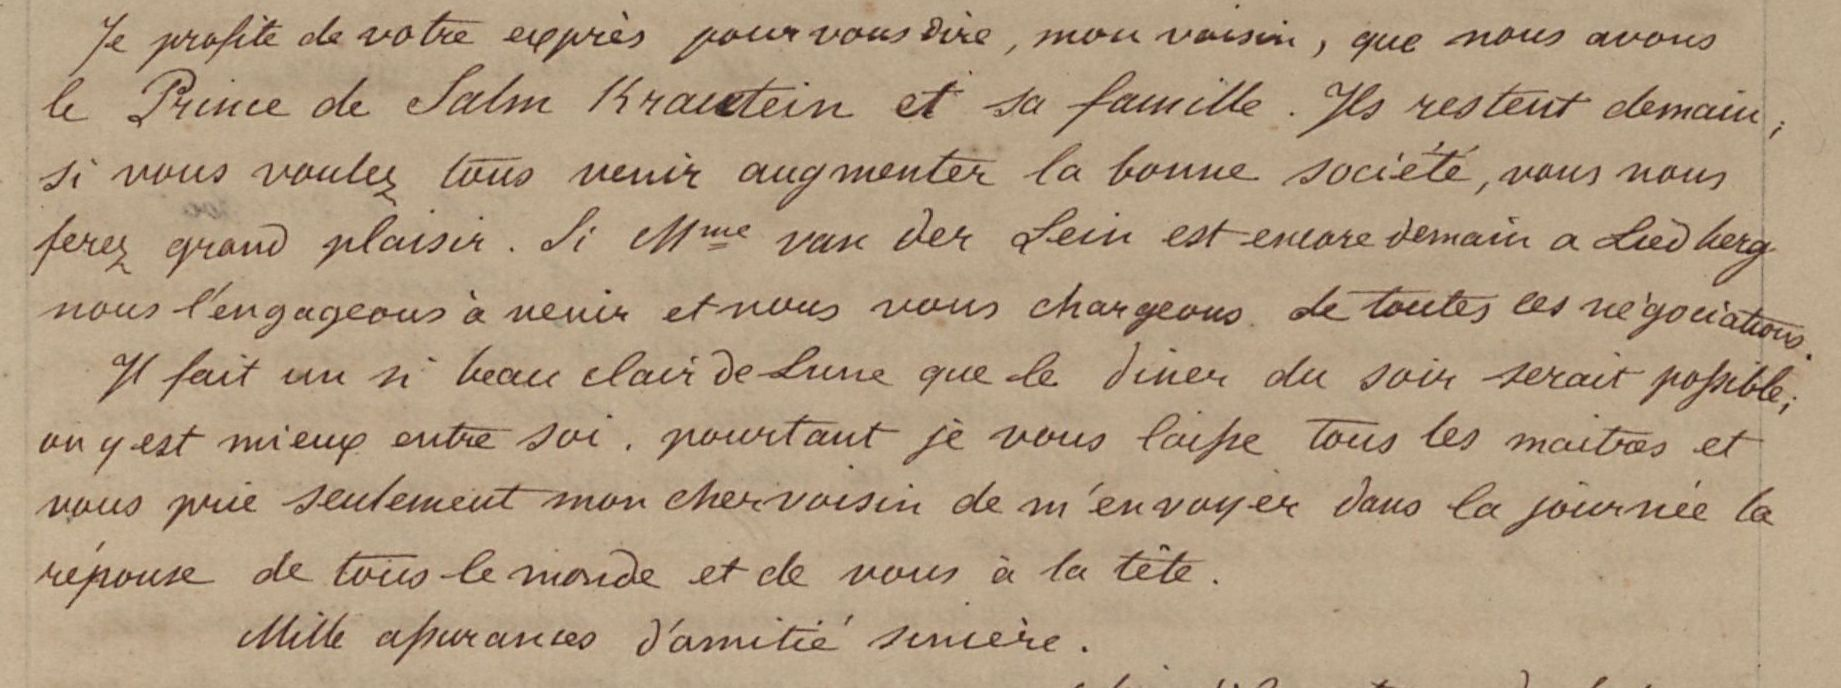
\includegraphics[width=11cm]{img/mainCdS02_Konv002_01-02_0065.jpg}
					\caption{Première main principale des recueils de la deuxième copie (\gls{lai}, détail du cliché CdS02\_Konv002-02\_0065.jpg).}
					\label{}
				\end{figure}
			
				Une main est particulièrement attestée dans la première moitié du premier volume~; elle est ici qualifiée de \og deuxième main principale\fg.
				
				\begin{figure}[!h]
					\centering
					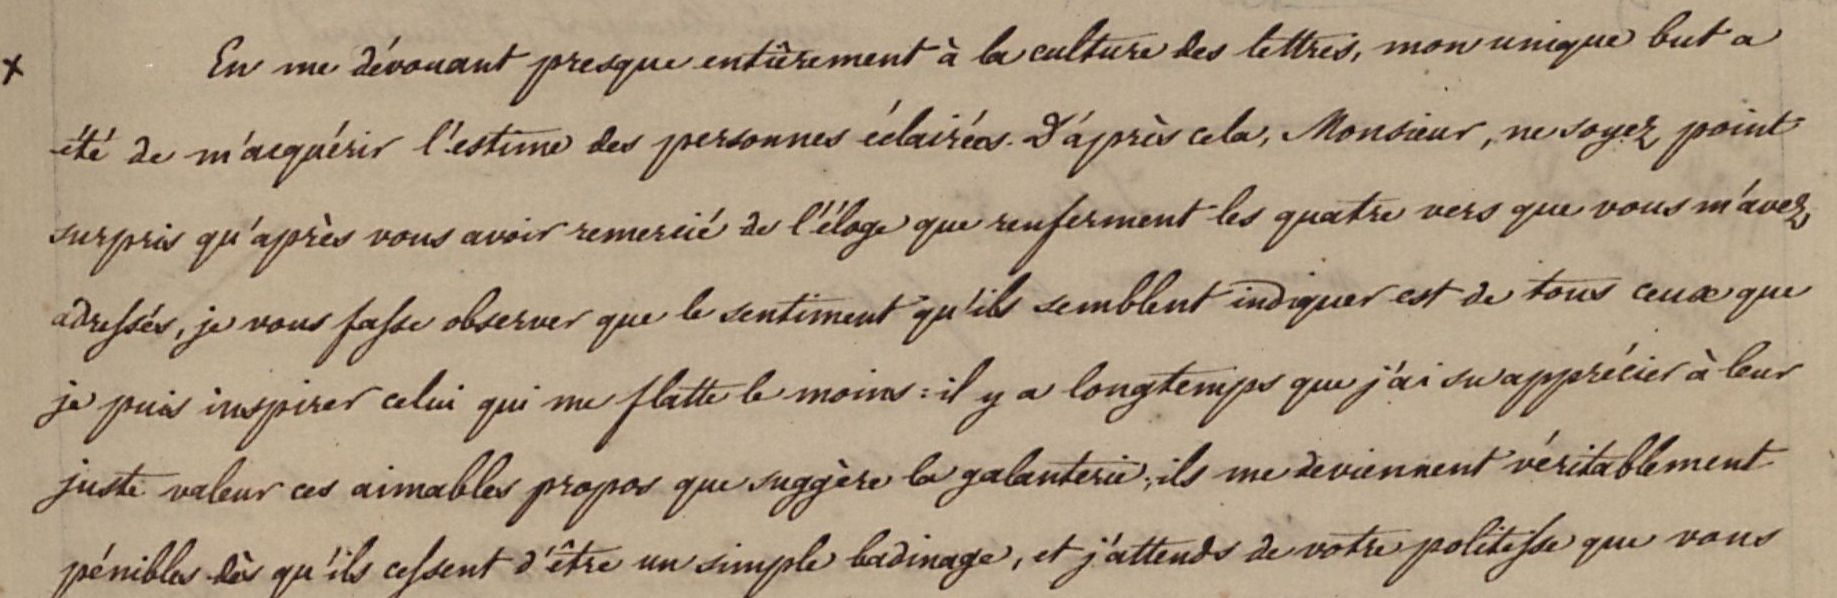
\includegraphics[width=11cm]{img/mainCdS02_Konv002_02-01_0030.jpg}
					\caption{Deuxième main principale des recueils de la deuxième copie (\gls{lai}, détail du cliché CdS02\_Konv002-01\_0030.jpg).}
					\label{}
				\end{figure}
			
				L'écriture qualifiée de \og troisième main principale \fg{} est sporadiquement attestée dans les trois volumes, mais a néamoins été identifiée sur presque 160 pages.
			
				\begin{figure}[!h]
					\centering
					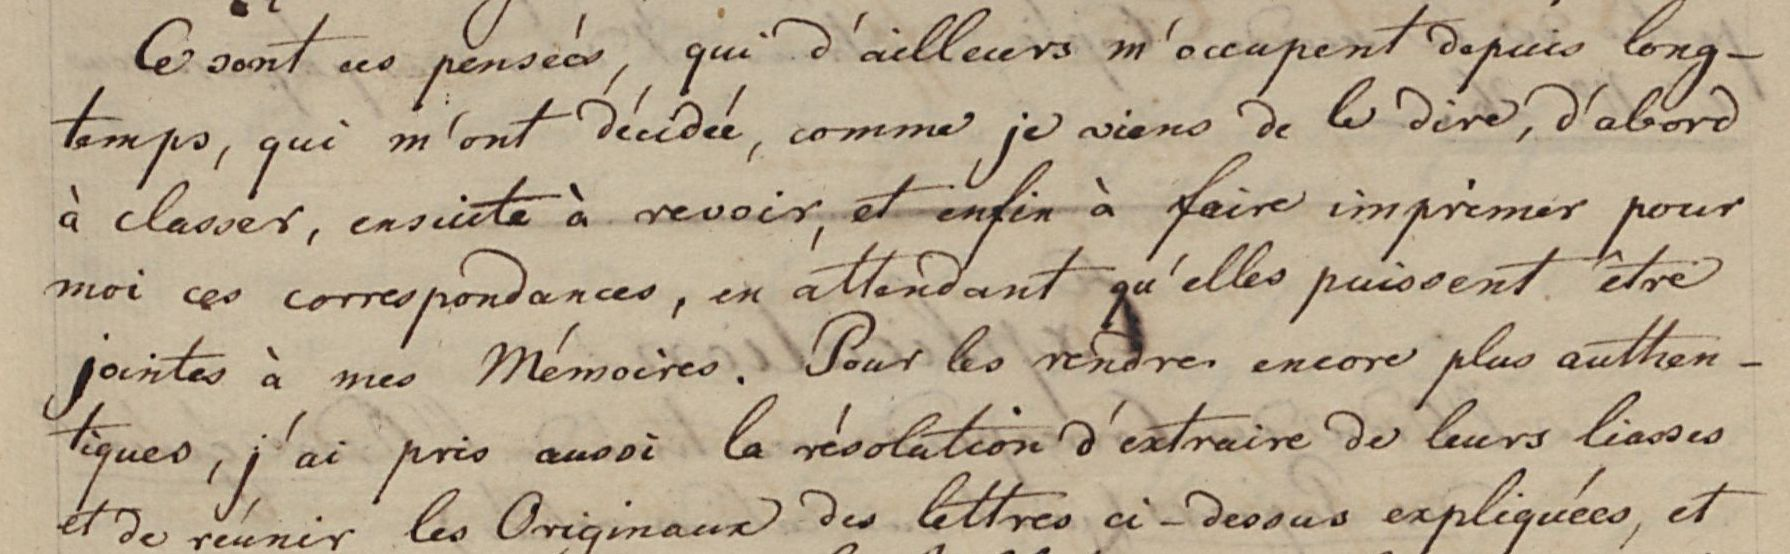
\includegraphics[width=11cm]{img/mainCdS02_Konv002_03-01_0006.jpg}
					\caption{Troisième main principale des recueils de la deuxième copie  (\gls{lai}, détail du cliché CdS02\_Konv002-01\_0006.jpg).}
					\label{}
				\end{figure}
					
				Les écritures du recueil de la correspondance adressée par J.P.E.~Martini à \gls{cds} ont également été analysées afin d'élargir la variété de notre corpus de tests. Deux mains y ont été distingués.
				
				\begin{figure}[!h]
					\centering
					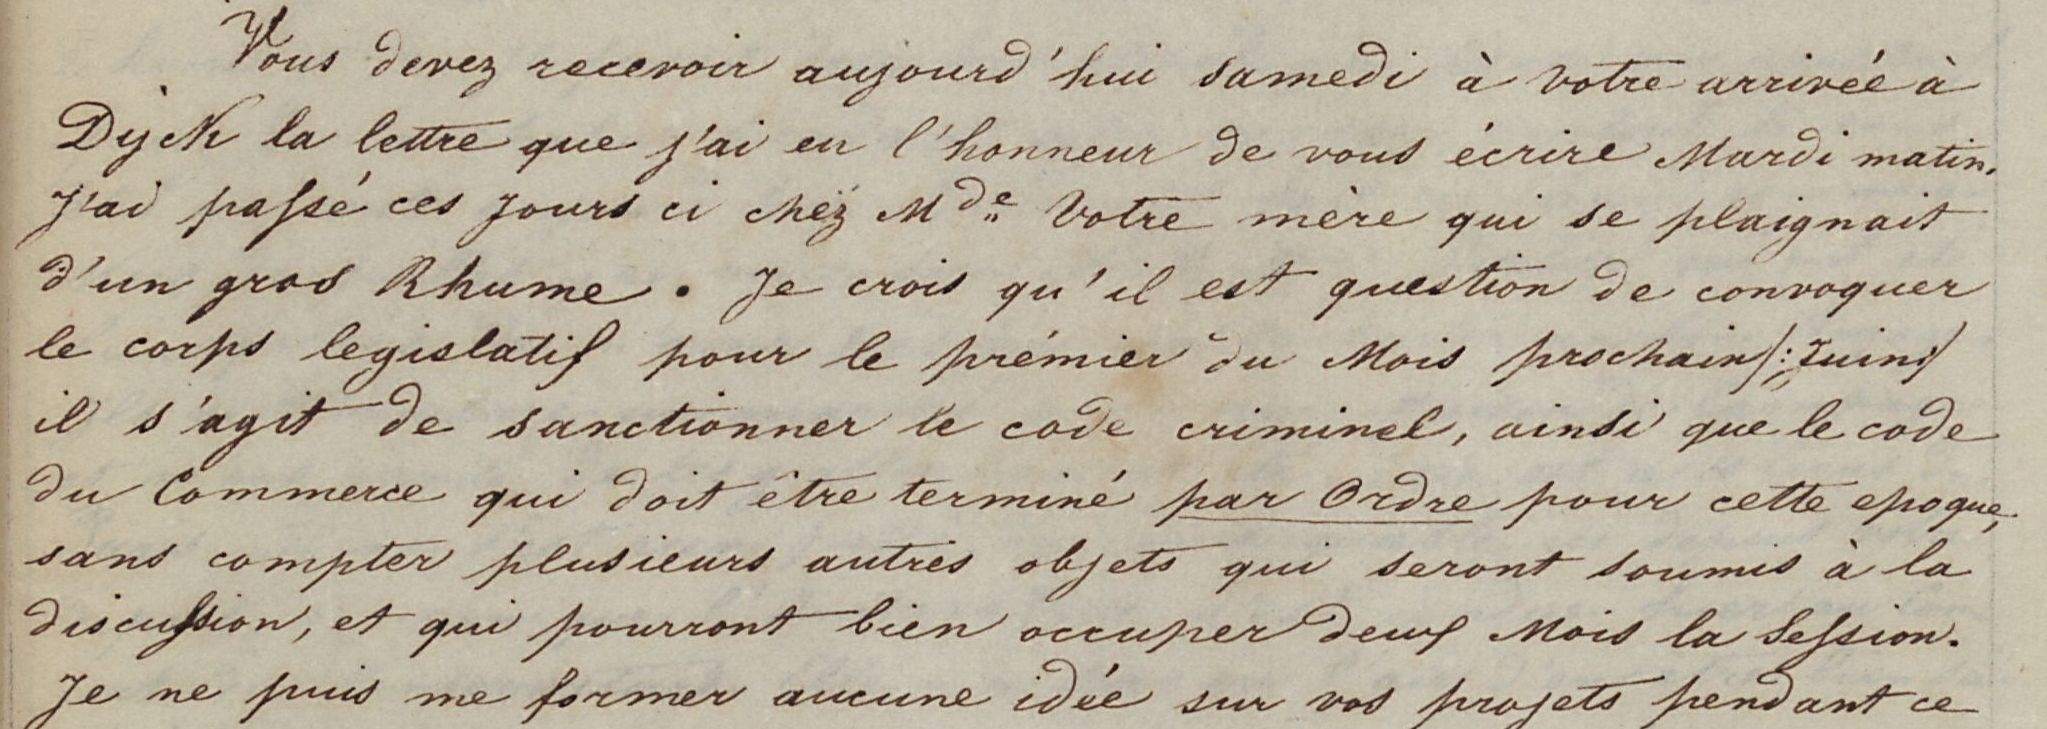
\includegraphics[width=11cm]{img/mainCdS02_Konv019_01-0002.jpg}
					\caption{Première main de la correspondance Martini (\gls{lai}, détail du cliché CdS02\_Konv019\_0002.jpg).}
					\label{}
				\end{figure}
				
				\begin{figure}[!h]
					\centering
					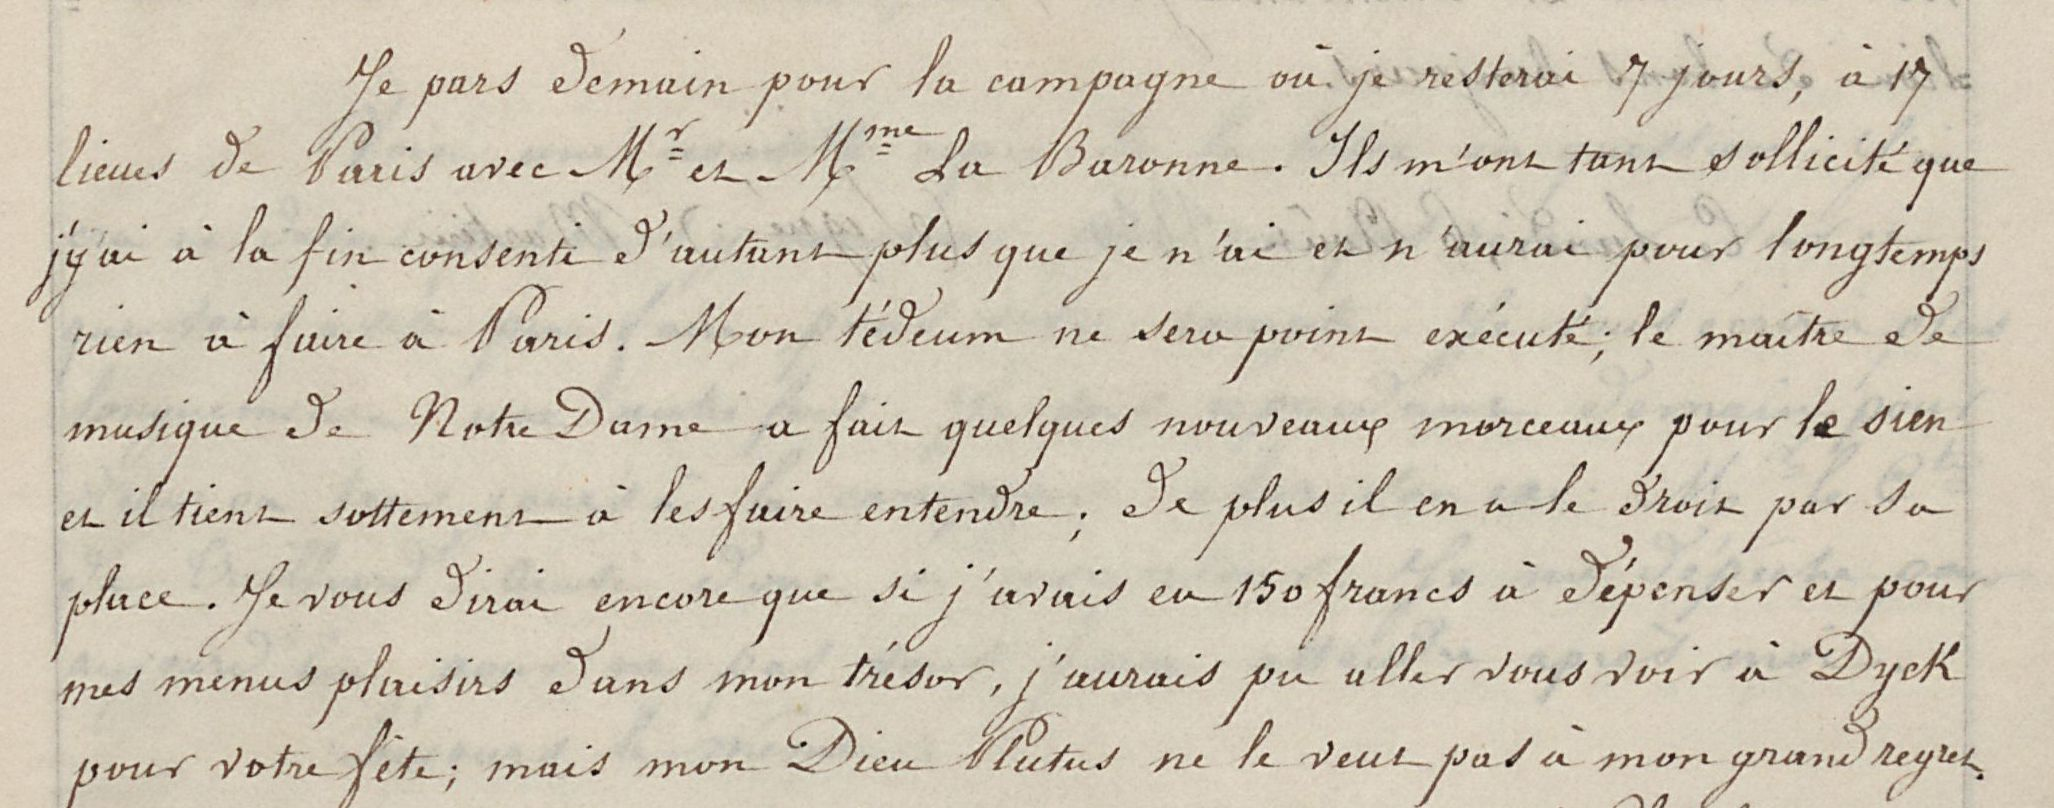
\includegraphics[width=11cm]{img/mainCdS02_Konv019_02-0036.jpg}
					\caption{Seconde main de la correspondance Martini (notice \cite{CdS19036037}).}
					\label{}
				\end{figure}
					
				On a privilégié pour les corpus de test et d'entraînement des modèles des reproductions favorables à une bonne reconnaissance de l'écriture, évitant en particulier les problèmes de transparence qui font ressortir au recto l'encre du verso (un problème assez présent dans la correspondance Martini).

			\subsection{L'écriture personnelle de C.~de Salm~: un défi paléographique}
				Concernant l'écriture personnelle de \gls{cds}, le site ne publie aucune lettre originale de sa main, mais 52 brouillons (\textit{Entwurf}). Entraîner un modèle de reconnaissance sur cette écriture suppose un travail délicat de transcription d'une écriture particulièrement cursive.
				
				\begin{figure}[!h]
					\centering
					\includegraphics[width=15cm]{img/CdS-b1-00k3-0_orig.jpg}
					\caption{Écriture autographe de \gls{cds} (notice \cite{C11S92047049}, transcription \textit{infra}, p.~\pageref{trans-C11S92047049}).}
					\label{}
				\end{figure}
				
				Nous avons tenté l'expérience de produire des vérités de terrain pour l'entraînement d'un modèle de reconnaissance propre à cette écriture, mais les résultats des premiers tests se sont révélés décourageants~: la meilleur acuité obtenue ne dépassait pas 44\%
				\footnote{Résultat obtenu rétrospectivement avec le modèle que nous avons entraîné sur quatre mains~: cds\_lectcm\_04\_mains\_01.mlmodel.}.
				
				Par ailleurs, les difficultés rencontrées pour transcrire des pages de l'écriture de \gls{cds} ont été importantes. Il a donc fallu renoncer à cette expérience, au risque d'y passer un temps long pour un résultat douteux.
				
				Faute de vérités de terrain dignes de ce nom, nous donnons en annexe à ce travail les transcriptions de deux extraits de lettres
				\footnote{Voir infra, \ref{autographes}, p.~\pageref{autographes}.}.
		
			\subsection[Préparer le traitement d'un dossier]{Préparer le traitement d'un dossier~: méthodologie de sélection des pièces publiées}
				L'archive photographique de la correspondance de \gls{cds} comporte des documents non inventoriés et des éléments inventoriés mais non publiés. Un script de contrôle des données a été écrit pour dresser la liste des notices d'inventaire mais dont les données n'ont pas été validées pour la publication\cite{biayDonneesNonPublieesPy2022}~; il permet d'afficher ces données dans un fichier au format \gls{json}, en donnant la liste des images concernées.
				
				À ce titre tous les dossiers ne sont pas logés à la même enseigne. Par exemple des images du premier volume de la seconde copie\cite{CdS02001330} ont été inventoriées sans être publiées. En revanche, pour le deuxième volume\cite{CdS02001369}, les images non publiées n'ont pas non plus été inventoriées~; tout un lot de textes contenus dans les images de ce volume sont donc dépourvus de données d'inventaire. 
				
				Cette situation, certainement fondée sur des critères de pertinence (en particulier celui de ne pas inventorier les copies de lettres dont les originaux ont déjà leur propre notice), représente un obstacle à la gestion automatisée des transcriptions qui peuvent être constituées d'un mélange de pièces non inventoriées (et donc dépourvues de toutes données descriptives) et de pièces inventoriées (ces dernières pouvant être associées à une adresse web déjà publiée et d'autres non). Prenons l'exemple de la figure \ref{non-invent-58}. Cette photographie contient la fin d'une lettre\footcite{CdS02057058}, le début d'une autre\footcite{CdS02058059}, et entre les deux une lettre non inventoriée, dont le titre se situe en haut de la page de droite.
				
				\begin{figure}[!h]
					\centering
					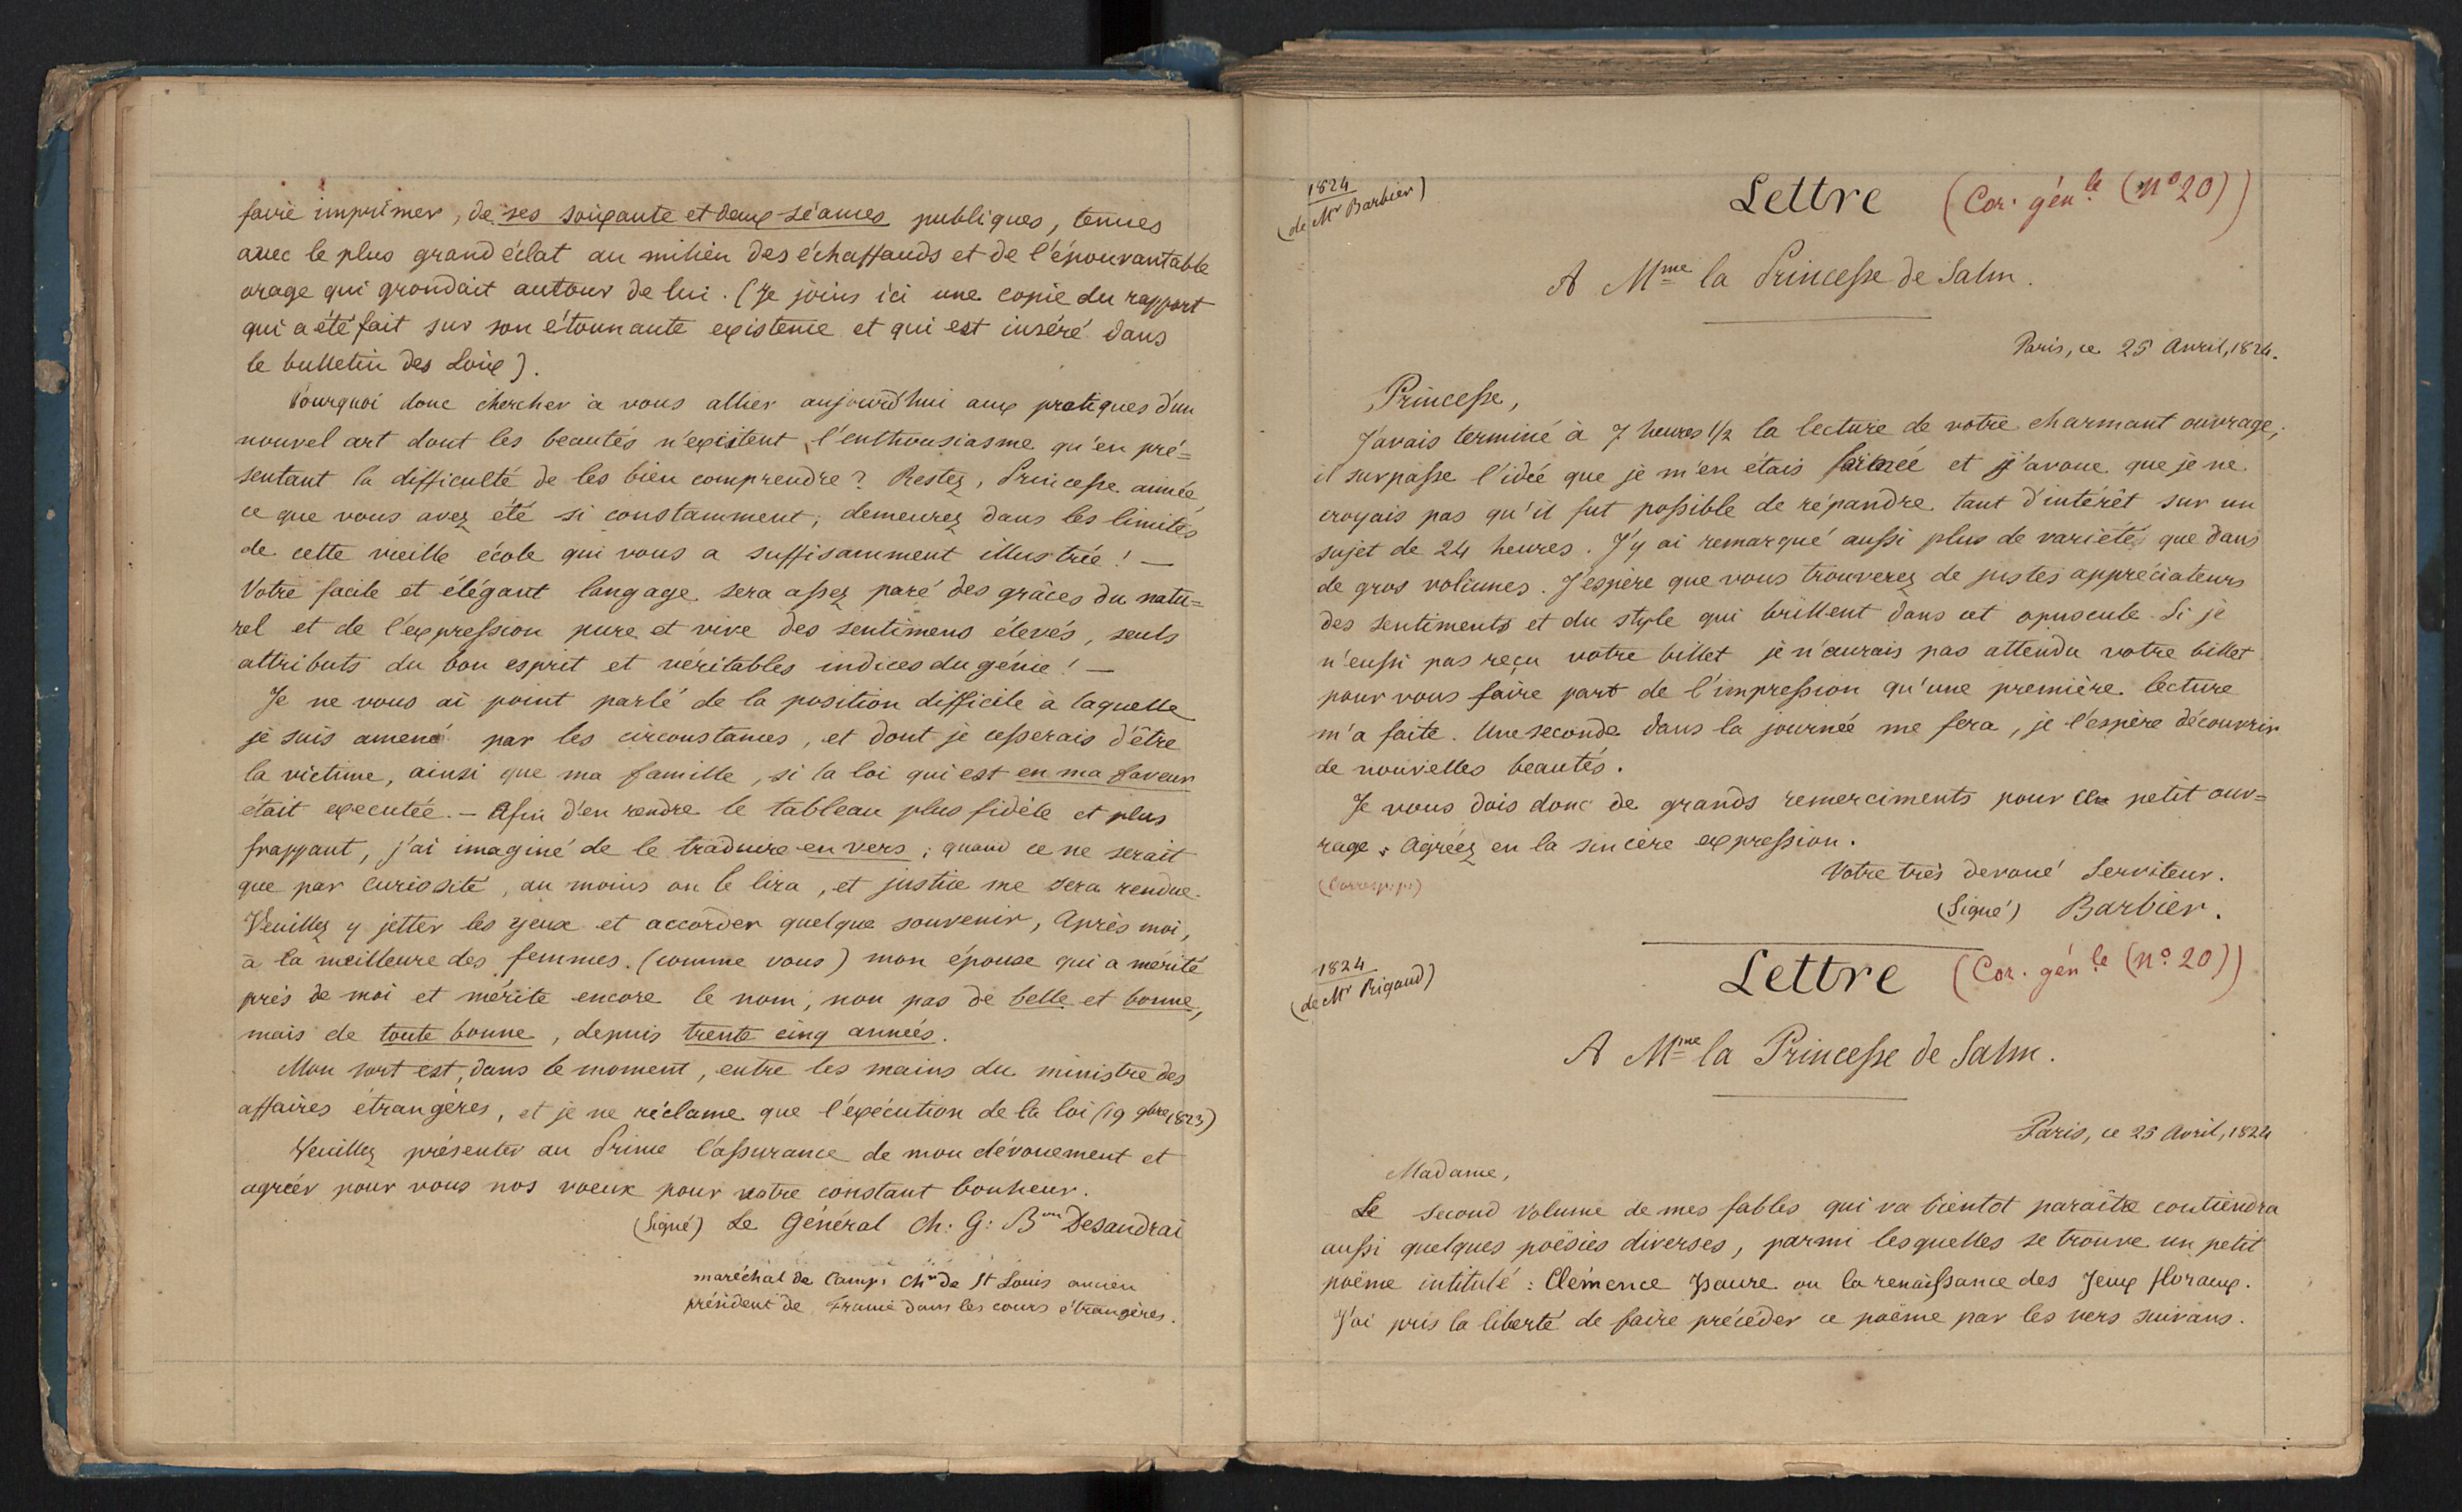
\includegraphics[width=15cm]{img/CdS02_Konv002-03_0058.jpg}
					\caption{Image contenant trois lettres dont l'une n'est pas inventoriée (cliché~: CdS02\_Konv002-03\_0058.jpg)}
					\label{non-invent-58}
				\end{figure}
				
				Admettons que l'on ne souhaite éditer que les lettres inventoriées. Les données de l'inventaire permettent d'établir d'une part que la première lettre attestée dans cette image commence à l'image précédente et que d'autre part l'inventaire connaît une seconde lettre dont le titre se situe dans cette image. Si l'on ne procède pas d'une manière ou d'une autre à l'élimination préalable de la lettre non inventoriée, il faudra non seulement corriger la {segmentation} et la transcription d'une lettre que l'on ne souhaite pas conserver dans l'encodage final (surcroît de travail inutile), mais aussi encoder à la main, pour la transcription de chaque lettre, toutes les données descriptives issues de l'inventaire, car aucun moyen de permettra alors de déterminer si le titre de la seconde lettre inventoriée sur la page est celui situé en haut de la page de droite ou s'il s'agit de celui situé en bas de la page de droite.
						
				Face à ce problème et à la présence (inégale selon les dossiers) de données non publiées dans l'inventaire, le parti a été pris de n'engager dans notre chaîne de traitement que des documents non seulement inventoriés mais dont les notices ont en outre été publiées sur le site \url{http://constance-de-salm.de}.
				
				Il va de soi que la chaîne de traitement peut être conduite sans tenir compte de cette étape de sélection des pièces. Si le parti devait être pris de transcrire l'intégralité d'un recueil sans distinction des pièces inventoriées et de celles qui ne le sont pas, il suffirait simplement de passer outre cette étape.
				
				La sélection des pièces est donc une étape importante du début de la chaîne de traitement que l'on a élaborée dans le cadre de ce stage. Un \textit{notebook} lui a été consacré\footcite{biayPreparerTraitementDossier2022}. Après l'étape préliminaire de l'import local et de la conversion des images au format Jpeg (afin de ne pas travailler avec le format Tiff, trop lourd), il est nécessaire d'établir la liste des images qui sont associées à une notice publiée de l'inventaire. Nous avons pour cela écrit un script python\footcite{biayDonneesImagesPy2022} qui analyse les noms des fichiers convertis et importés localement, croise ces noms avec les données de l'inventaire et écrit en sortie un fichier \gls{json} qui liste (entre autres informations), pour chaque notice l'inventaire contenant l'une des images du dossier, l'URL de cette notice sur le site \url{https://constance-de-salm.de} et la liste complète des images attachées à cette notice
				\label{donnees-images}
				\footnote{Le fichier donne par ailleurs la liste des images qui ne sont liées à aucune notice de l'inventaire, ainsi qu'une présentation des mêmes données d'association image-notice, mais cette fois par image et non par notice, et ce afin de permettre le contrôle visuel des zones de texte à transcrire (cf.~\textit{infra}, \ref{controle-segmentation-lettres-inventoriees}, p.~\pageref{controle-segmentation-lettres-inventoriees})}.
				
				Une fois le dossier analysé et le fichier produit, les commandes que nous avons écrites dans le \textit{notebook} permettent de n'importer dans le dossier de travail que les images correspondant à une notice de l'inventaire. Dans le cas spécifique illustré par la figure \ref{non-invent-58} d'une image contenant un mélange de pièces inventoriées et de pièces non inventoriées, c'est au stade de la {segmentation} que l'élimination des lettres non inventoriées est proposée (voir \textit{infra}, p.~\ref{controle-segmentation-lettres-inventoriees}).
							
			\subsection[Transkribus ou eScriptorium~?]{Transkribus ou eScriptorium~? Fonctionnalités avancées \textit{versus} science ouverte}
				Au moment du présent stage, les deux principales applications permettant de procéder à la transcription automatique des écritures manuscrites sont eScriptorium et Transkribus.
				
				Différentes considérations peuvent conduire à opter pour l'une ou l'autre de ces applications\footnote{Nous avons assisté le 9 mai 2022 à l'atelier organisé au sein du Data-Lab de la \gls{bnf} et dont le programme est détaillé dans le billet d'\cite{jacquotTranskribusEScriptoriumTranscrire}.}. Deux facteurs nous apparaissent particulièrement déterminant pour fonder un tel choix~:
				
				\begin{enumerate}
					\item Sur le plan théorique~: l'observance des principes de la science ouverte~;
					\item Sur le plan pratique~: les compétences d'ingénierie des personnes chargées de mener la campagne de transcription.
				\end{enumerate}
				
				Considérons dans un premier temps le plan pratique.
				
				L'écosystème applicatif Transkribus est celui qui propose le plus grand choix de services, tant pour les utilisateurs ayant des compétences d'ingénierie élevées (logiciel Expert Client) que pour les néophytes (Transkribus Lite). Conjuguées à la facilité de prise en main de Transkribus Lite, les fonctionnalités de gestion des versions de transcription offertes par Transkribus Expert Client rendent cet écosystème le mieux à même d'héberger des campagnes de transcription de grande ampleur, faisant appel à de multiples transcripteurs, voire à de la production participative (ou \textit{crowdsourcing}).
				
				L'application eScriptorium, à un stade de développement moins avancé\footcite{stokesEScriptoriumVREManuscript2021}, avec une interface dotée de moins de fonctionnalités que Transkribus (gestion des versions de transcription, annotation du texte), mobilise davantage de compétences d'ingénierie. En revanche, la gratuité totale de son utilisation et surtout la culture de science ouverte portée par la communauté qui développe et utilise eScriptorium rendent cette application tout à fait adéquate aux projets impliquant un petit nombre de transcripteurs ayant une bonne culture d'ingénierie au préalable, notamment au sein d'institutions désireuses de promouvoir la science ouverte.
				
				En effet, pour approfondir ce dernier point, la communauté active autour du développement et de l'utilisation de l'interface eScriptorium (elle même fondée sur le logiciel libre Kraken\footcite{KrakenDocumentation}), promeut les principes de la science ouverte de multiples manières (développement \textit{open-source}, respects de standards des formats numériques, ouverture des données de modèles, de vérités de terrain, développement d'outils auxiliaires à la transcription, à la gestion de fichiers, propositions de standards d'annotation). La possibilité de réutiliser et modifier librement le code source garantit une grande pérennité d'utilisation de ces applications et donc pour les projets qui y font appel. Un projet dépendant d'un écosystème logiciel clos tel que Transkribus court en effet le risque de ne plus pouvoir être mené en cas de défaillance de cet écosystème. Un logiciel libre installé localement pourra en revanche être maintenu et réparé, et le projet de se poursuivre une fois l'écueil franchi.
				
				L'ouverture des données (en particulier des données d'entraînement des modèles) est également décisive pour une politique de science ouverte appliquée à l'apprentissage machine. Cette technologie repose sur la consitution de données d'entraînement. Il en découle naturellement que ces données déterminent, conditionnent les résultats obtenus par les modèles entraînés (quelles images ont été choisies, quels textes ont été transcrits pour parvenir à tel résultat). Pour comprendre le fonctionnement de ces modèles et leurs performances, il faut donc disposer d'une archive des données d'entraînement~; celles-ci doivent être exposées de manière transparente, et ainsi pouvoir être critiquées, analysées ou réutilisées. Ainsi, le logiciel Kraken permet (techniquement) et la communauté eScriptorium encourage (politiquement) la publication et le partage des vérités de terrain (qui sont les véritables données brutes d'entraînement) ainsi que des modèles eux-mêmes\footcite{chagueHTRUnitedMutualisonsVerite2021}.
				%COMPLPOS Dimension écologique : L'apprentissage machine est un processus long et gourmand en énergie, il est donc essentiel de pouvoir en partager les bénéfices ; or il n'est pas possible d'exporter un modèle entraîné sur Transkribus
				
				On peut ajouter à cette considération sur le transparence des données le haut degré de souplesse requis par les projets d'édition scientifique. Que l'on prenne en considération les spécificités des sources éditées, les critères d'édition choisis par les chercheurs ou encore les finalités de ces projets, ces derniers impliquent une multiplicité de décisions incompatibles avec l'utilisation de solutions logicielles clé en main. Les besoins particuliers de la recherche sont ainsi beaucoup mieux servis par l'emploi de briques logicielles indépendantes, modulables, entre lesquelles peuvent s'échanger les données dans des standards bien établis, plutôt que par le recours à des suites logicielles performantes mais aux fonctionnalités déterminées par une communauté de développement extérieure au projet. Le risque est en effet immense de devoir reconsidérer les attendus du projets à la découverte soudaine d'une fonctionnalité manquante ou plus souvent encore de l'impossibilité de personnaliser un mode d'expression des données\footcite{stokesEScriptoriumVREManuscript2021}.
				
				Pour l'ensemble de ces raisons, nous avons opté pour l'utilisation d'eScriptorium et de Kraken dans le cadre de ce stage. Le flux de travail pourra sembler complexe à un utilisateur peu aguerri en matière d'ingénierie, mais en contrepartie une documentation fonctionnelle pas à pas a été rédigée grâce à la technologie du \textit{Jupyter notebook} qui permet en toute théorie de mener l'intégralité des tâches que l'on a experimentées avec une expertise réduite.
							
				Dans ce genre de configuration, une assistance pourra être requise pour l'étape la plus délicate en termes d'ingénierie~: l'installation des applications nécessaires à la conduite du projet, celle d'eScriptorium étant le point le plus critique et l'installation des applications en langage Python pouvant également poser quelques difficultés. Nous avons en effet utilisé eScriptorium à partir d'une installation locale\footnote{La démarche est expliquée sur la page suivante~: \cite{DockerInstallInstallation}.}, faisant appel aux seules ressources d'un ordinateur portable, à savoir sans serveur ni carte graphique externe\footnote{L'ordinateur utilisé est doté d'un processeur 11th Gen Intel Core i7-1165G7 @ 2.80GHz × 8 et d'une mémoire vive de 15,4 GiB.}. Cette méthode nous a permis de procéder à des entraînements de modèle à partir de petits volumes de vérités de terrain. Si des entraînements plus massifs s'avéraient nécessaires, il serait alors impératif de se tourner vers une infrastructure dotée de plus grandes capacités de calcul, ce que, par exemple, un partenariat entre le \gls{dhi} et le projet \gls{cremma} rendrait possible.
						
		\section[La {segmentation}]{La {segmentation}~: reconnaissance des zones de texte et des lignes d'écriture}
			\label{lieu-segmentation}
			
			La {segmentation} est une étape indispensable à la réalisation d'une reconnaissance automatique de l'écriture manuscrite. Il s'agit de l'étape la plus problématique, car les possibilités d'entraînement de modèles de {segmentation}, permettant d'automatiser le processus, recquièrent beaucoup plus de données d'entraînement pour des résultats souvent médiocres, contrairement à la reconnaissance de l'écriture elle-même.
			
			Cette section décrit les enjeux de cette opération et relate les expériences de {segmentation} qui ont été réalisées à partir des recueils de la correspondance de \gls{cds}.
						
			\subsection{Principes et enjeux}
				Contrairement à certains logiciels d'\gls{ocr}, qui procèdent directement à une reconnaissance optique caractère par caractère, tous les logiciels d'\gls{htr} fonctionnent en appliquant la reconnaissance optique au niveau de la ligne d'écriture (principe dénommé en anglais \textit{line-wise text recognition})\footcite{stokesEScriptoriumVREManuscript2021}. Cette technologie fonctionne sur la base d'un module d'analyse de la mise en page (\textit{layout analysis module}) qui fonctionne indépendamment du type d'écriture rencontré, rendant ainsi possible pour une application comme Kraken de travailler sur tous les types d'écritures (alphabétiques et autres). Les logiciels Transkribus et Kraken reconnaissent les lignes de base des écritures (\textit{baselines}) et peuvent ainsi repérer des zones de texte où qu'elles se situent dans une page et quelque soit leur orientation. 
				
				Les capacités de l'algorithme par défaut de l'application Kraken ont été éprouvées à travers l'utilisation du logiciel eScriptorium. Les recueils de copies de lettres, présentant la particularité d'une mise en page incluant des manchettes aux lignes écrites en diagonale pour chaque lettre, représentaient un intérêt singulier.
				
				\begin{figure}[!h]
					\centering
					\includegraphics[width=15cm]{img/CdS02_Konv002-02_0065-seg-auto-detail.jpg}
					\caption{Segmentation par le modèle par défaut de Kraken (\gls{lai}, détail du cliché CdS02\_Konv002-02\_0065.jpg).}
					\label{seg-defaut-65}
				\end{figure}
			
				On constate la difficulté de ce modèle standard à situer les lignes de base du texte écrit en diagonal, en haut à gauche de la page. En revanche et pour l'essentiel, le modèle a parfaitement détouré (en vert) deux régions d'écriture (la manchette et le corps de la lettre)~; il a en outre très bien repéré toutes les lignes d'écriture horizontales.
				
				Mais si la reconnaissance correcte des lignes d'écriture garantit a propri une bonne transcription des lettres, éditer les lettres d'un tel recueil implique une autre opération~: distinguer les lettres les unes des autres. En effet, et c'est l'une des caractéristiques de la mise en page de ces recueils de copie, les lettres y sont copiées à la suite les unes des autres, séparées par des titres. De plus, une lettre commence souvent sur une double page pour se terminer sur la suivante, son texte se partageant entre deux photographies. Si l'on veut éviter la tâche fastidieuse de reconstituer à la main le texte des lettres à partir des transcriptions automatiques de chaque photographie (en réunissant par copier-coller ces différentes parties dans un fichier commun), il devient crucial de structurer la transcription du texte contenu dans chaque image par le repérage dans le flux de texte d'éléments permettant cette structuration, à savoir les titres.
				
				Rien n'est plus évident à l'œil humain que de voir un titre et de comprendre qu'il marque la fin d'une lettre et le début d'une autre. Or le modèle de {segmentation} par défaut de Kraken ne réalise pas cette coupure par lui-même. On le voit sur l'image suivante, la même zone verte englobe la fin d'une lettre et le début d'une autre.
				
				\begin{figure}[!h]
					\centering
					\includegraphics[width=15cm]{img/CdS02_Konv002-02_0073-seg-auto-detail.jpg}
					\caption{Segmentation par le modèle par défaut de Kraken (notice~: \cite{CdS02073}).}
					\label{}
				\end{figure}
				
				La {segmentation} des pages et des lignes d'écriture pose donc une problématique. Dans quelle mesure est-il possible d'automatiser ce processus sachant qu'il est primordial que les lignes d'écriture soient correctement reconnues, qu'il est très important de pouvoir repérer les titres des lettres et que de surcroît, il n'est pas raisonnablement envisageable de créer un modèle totalement personnalisé. En effet, on a pu faire l'expérience que tenter d'entraîner un modèle à partir de zéro ne permet même pas d'aboutir à une bonne reconnaissance des lignes. La seule méthode efficace consiste donc à tirer le meilleur profit des performances du modèle standard et à tenter d'améliorer ces performances pour le rendre plus spécifique à la mise en page de ces copies de lettres.
				
				Ces considérations générales étant posées, on se soit d'approfondir les problèmes dotn les bases viennent d'être posées~: le comportement du modèle standard de {segmentation} de Kraken à l'égard des particularités de la mise en page des sources du projet d'une part, les possibilités de structuration offertes par cette étape de la {segmentation} en vue de l'encodage de ces lettres au format \gls{tei}, finalité du présent travail.
					
			\subsection{Définir une structure de document idéale en vue de l'édition}
				Il est important de prendre en considération la morphologie que devra prendre l'encodage final des lettres avant même de se lancer dans l'évaluation des possibilités de {segmentation} automatique des pages. En effet, l'étape de la {segmentation} consiste à annoter (manuellement ou, si possible, automatiquement) des zones ou régions d'écriture et les lignes qui y sont comprises. Si l'on associe, par exemple, à la ligne qui dans l'image contient le texte \textit{Signé Constance de Salm} l'information sémantique selon laquelle il s'agit de la signature d'une lettre, il devient possible d'encoder automatiquement le texte comme étant une signature dans l'édition numérique finale.
				
				Des propositions d'encodage extrêmement complètes pour l'édition de correspondances ont été formulées dans les \textit{Guidelines} du projet DAHN\footcite{chiffoleauCorrespondenceGuidelines2022}. En lien avec ces propositions d'encodage, F.~Chiffoleau a en outre élaboré une ontologie des régions d'écriture pour les correspondances en langue française pour le \siecle{xx}~siècle \footcite{chiffoleauCorrespondanceLangueFrancaise2021}, dans le cadre du projet \gls{segmonto}\footcite{gabaySegmOntoCommonVocabulary2021}. Voici les types de régions d'écriture dont l'application aux sources du présent projet pouvait être pertinente~:
				\selectlanguage{english}
				\textit{\begin{itemize}
					\item \textbf{Main};
					\item \textbf{Title};
					\item \textbf{Signature};
					\item \textbf{Numbering}: numbering at the top of the letter;
					\item \textbf{Salute};
					\item \textbf{Dateline}: place and date of writing for the letter;
					\item \textbf{Additions}: handwritten additions outside of the main text.
				\end{itemize}}
				\selectlanguage{french}
				
				Par ailleurs, les réflexions suscitées par ces catégories lors du point d'étape du 22 avril 2022\footnote{On participé à cette discussion Anne Baillot, Floriane Chiffoleau, Pauline Spychala, Evan Virevialle et moi-même.} ont fait émerger l'idée d'une simplification de cette ontologie par régions autour de trois notions principales marquant l'ouverture, le corps et la fin de la lettre:
				\textit{\selectlanguage{english}
				\begin{enumerate}
					\item Opener;
					\item Main;
					\item Closer.
				\end{enumerate}}
				\selectlanguage{french}
				
				Il fallait en outre envisager l'annotation des éléments périphériques (annotations, annotations et systèmes de numérotation divers)~:
				\textit{\selectlanguage{english}
				\begin{enumerate}
					\item Annotations;
					\item Numbering.
				\end{enumerate}
				\selectlanguage{french}}
				
				Restait à savoir (et ça n'était pas la moindre question) si un modèle de {segmentation} serait capable d'identifier ces régions d'écritures de manière automatique.
    
		    \subsection{Problèmes posés par l'espacement des lignes}
				La mise en page des lettres dans les recueils de copie répond à des principes clairs pour l'œil humain~; il présente en revanche d'importantes variations métriques dans l'espace de la page. On a déjà pointé précédemment un problème de taille~: les lettres sont écrites les unes à la suite des autres, et le modèle de {segmentation} par défaut de Kraken ne se montre pas capable de les séparer de lui-même.
				
				Ce modèle procède à l'évaluation de l'espacement entre les régions d'écritures~: il fusionne dans une seule région les lignes qui lui semblent suffisamment proches~; il assigne en revanche à des régions distinctes les lignes qui lui semblent suffisamment éloignées. On a vu que cette appréciation lui permet de distinguer la manchette des lettres, caractéristique de ces recueils de copie (voir \textit{supra}, figure~\ref{seg-defaut-65}, p.~\pageref{seg-defaut-65}). L'exemple illutré par la figure \ref{seg-opener-193} montre la capacité de ce modèle à distinguer l'ouverture de la lettre (\textit{opener}) en réunissant dans une région cohérente et indépendante le titre de la lettre, le lieu et la date (ainsi qu'une annotation de type catalographique écrite en rouge).
				
				\begin{figure}[!h]
					\centering
					\includegraphics[width=15cm]{./img/CdS02_Konv002-02_0193-detail-01.jpg}%
					\caption{Mise en page aérée au début d'une lettre (\gls{lai}, détail du cliché CdS02\_Konv002-02\_0193.jpg).}%
					\label{seg-opener-193}
				\end{figure}
			
				En revanche, dans l'exemple illustré par la figure \ref{seg-glob-46}, les lignes d'écriture sont tellement peu espacées sur l'axe veritcal qu'une seule région de texte réunit le titre, la date et le corps de la lettre.
			
				\begin{figure}[!h]
					\centering
					\includegraphics[width=15cm]{./img/CdS02_Konv002-02_0046-detail.jpg}%
					\caption{Mise en page resserrée au début d'une lettre (\gls{lai}, détail du cliché CdS02\_Konv002-02\_0046.jpg).}%
					\label{seg-glob-46}%
				\end{figure}
				
				La reconnaissance de la fin d'une lettre (dont la signature alignée à droite de la page est l'élément le plus récurrent) est encore plus délicate, car elle ne se manifeste jamais par un élément visuellement massif comme un titre. De plus, les mêmes différences de comportement s'observent selon l'espacement des lignes~: dans quelques cas rares, comme celui illustré par la figure \ref{seg-signaure-71}, la signature peut être distinguée en une région spécifique, mais dans la très grande majorité des cas, elle est perçue comme appartenant à la même région que le corps de la lettre.
				
				\begin{figure}[!h]
					\centering
					\includegraphics[width=15cm]{./img/CdS02_Konv002-03_0071-signature.jpg}%
					\caption{Mise en page aérée en fin de lettre (notice~: \cite{CdS02070071}).}%
					\label{seg-signaure-71}%
				\end{figure}
				
				Ces premières observations suggèrent qu'entraîner un modèle à reconnaître les différentes parties d'une lettre sous forme de régions d'écritures distinctes (catégorisées ci-dessus \textit{opener}, \textit{main} et \textit{closer}) s'annonce difficile. D'autres observations relatives à la numérotation des lignes ont confirmé les inconvénients de cette méthode.
				
			\subsection{Gérer la numérotation des lignes}
				La numérotation des lignes de texte est une opération essentielle de la {segmentation}. Rien ne pourrait être fait de la transcription automatique du texte si les lignes n'étaient pas transcrites dans l'ordre de lecture. L'algorithme de {segmentation} par défaut de Kraken est bien entendu capable de numéroter les lignes selon les préférences de l'utilisateur, et dans le cas présent, de gauche à droite et de haut en bas.
				
				Paramètre important~: la numérotation des lignes dépend de la position des régions qui les englobent dans l'image analysée. Ainsi, la mise en page particulière des documents et le découpage du texte par régions peut jouer un rôle déterminant dans l'ordre des lignes. L'expérience a pu en être faite en remodelant de différentes manières les {segmentation}s automatiquement produites le modèle par défaut de Kraken.
				
				Or les problèmes de numérotation ont été nombreux lors de ces tests. Comme le montre la figure \ref{comp-av-opener-ln-reg-193}, issue du vol.~2 de la seconde copie\footcite{CdS02001369}, obtenir une bonne numérotation des lignes de titre s'est révélé problématique dès lors que l'on souhaitait isoler ces titres dans une région propre (\textit{opener}). On observe en effet dans cet exemple que le titre situé sur la page de gauche est numéroté 23 et 24~; il ne s'intercale donc pas correctement entre les lignes de la manchette (10 et 11) et les lignes du corps de la lettre (à partir de 12). Le même phénomène s'est produit dans cet exemple pour les trois titres de la double page. Sachant que le titre est le seul élément sur lequel on puisse s'appuyer pour distinguer automatiquement le début et la fin des lettres (car il n'y a pas toujours de signature, pas toujours de manchette, pas toujours de date pour borner le texte des lettres), la mauvaise numérotation des lignes de titre est un énorme problème en vue de l'exploitation des \glspl{prédiction}~: sans intervention, les titres de chaque lettre de cette page se retrouveraient disposer à la fin du texte de leur lettre et ainsi passer pour le titre de la lettre suivante…
				
				Il est naturellement possible de corriger ces problèmes de numérotation de façon manuelle dans l'interface eScriptorium, mais il s'agit d'un travail fastidieux (chaque ligne doit être déplacée une par une) et hasardeux (le rechargement de la page peut rétablir la  numérotation d'origine.) Il fallait donc prévenir ce problème.
				
				\begin{figure}[!h]
					\centering
					\includegraphics[width=15cm]{img/comp-av-opener-ln-reg-CdS02_Konv002-02_0193.jpg}
					\caption{Exemple de numérotation à partir d'une {segmentation} distingant \textit{opener} et \textit{closer} (cliché CdS02\_Konv002-02\_0193.jpg).}
					\label{comp-av-opener-ln-reg-193}
				\end{figure}
			
				Une première solution a consisté à envelopper toutes les régions d'écriture dans une sorte de super-région, dessinée autour des autres régions précédemment définie~: la page. En liant les lignes d'écriture à la page qui les englobe, l'ordre de lecture de gauche à droite et de haut en bas assure une bonne numérotation des lignes~: on constate que les titres ont retrouvé leur juste numérotation.
				
				\begin{figure}[!h]
					\centering
					\includegraphics[width=15cm]{img/comp-av-opener-ln-pag-CdS02_Konv002-02_0193.jpg}
					\caption{Exemple de numérotation avec lignes liées à une région \textit{page} (cliché CdS02\_Konv002-02\_0193.jpg).}
					\label{annotation-page-66}
				\end{figure}
				
				Cette solution pouvait sembler prometteuse jusqu'au moment où il s'est agit d'examiner les fichiers \gls{alto} compilés par le logiciel eScriptorium, où la transcription des textes de la page se trouve structurée en fonction des régions d'écriture que l'on a définies. Le choix de lier les lignes d'écritures à la super-région \textit{page} les avait (logiquement) déconnectées de leurs propres régions~: le fichier se présentait avec des régions \textit{page} pleines de lignes d'écriture et des régions \textit{opener}, \textit{main}, etc. entièrement vides. Il devenait dès lors impossible d'exploiter les étiquettes données à ces régions d'écriture en vue de la réalisation de l'encodage des lettres~: les lettres ne pouvaient plus être distinguées les unes des autres. Il a donc fallu renoncer à emboîter des régions d'écriture pour résoudre les problèmes de numérotation. 
				
				La solution finalement apparue comme la seule possible consistait à simplifier la définition des régions d'écriture. Dans la figure \ref{comp-ss-opener-193}, la {segmentation} consiste à séparer les lettres les unes des autres et à distinguer la manchette (un choix que l'on a maintenu dans la mesure où le modèle par défaut de Kraken s'est montré capable d'opérer seul cette distinction). Toutes les parties de la lettre sont réunies dans une même région (sauf si la lettre se prolonge sur l'image suivante, naturellement). Cette option a non seulement permis de résoudre les problèmes de numérotation des titres, mais aussi de résoudre un autre problème de numérotation assez récurrent~: la ligne indiquant le lieu et la date de la lettre (numéros 14, 32 et 46 dans l'exemple en question) s'intercalait assez souvent entre la première et la seconde ligne du texte de la lettre. On a également observé dans un certain nombre de cas les deux premières lignes du texte numérotées en ordre inverse.
				
				\begin{figure}[!h]
					\centering
					\includegraphics[width=15cm]{img/comp-ss-opener-01-CdS02_Konv002-02_0193.jpg}
					\caption{Exemple de numérotation sans région de \textit{page} ni \textit{opener} (cliché CdS02\_Konv002-02\_0193.jpg).}
					\label{comp-ss-opener-193}
				\end{figure}
				
				On le voit dans l'exemple en question, il a également été choisi de ne pas distinguer de région \textit{closer} pour la signature des lettres. Après quelques tentatives d'entraînement de modèle de {segmentation} en ce sens, les résultats très mauvais que l'on a obtenus prouvaient avec assez de force que cette tentative était vouée à l'échec.
				
			\subsection{Définir une ontologie des régions et des lignes}
				Une fois arrêtés les principes généraux de la {segmentation}, il convient de définir une ontologie, à savoir la liste des types de régions et de lignes d'écriture que l'on entend appliquer à cette {segmentation}.
				
				Le choix a été fait d'inscrire cette définition des régions et des lignes suivant les principes de l'ontologie \gls{segmonto}. Déjà cité, le projet \gls{segmonto} propose un cadre conceptuel général pour ce genre de définition. Bien qu'orienté sur la description des manuscrits médiévaux et des premiers imprimés, il met en avant les catégories les plus génériques possibles (\textit{main}, \textit{margin}, \textit{numbering}, etc.) ainsi que des solutions de personnalisation, afin de permettre à tout type de projet d'exprimer ses besoins d'annotation de régions et de lignes d'écriture dans un cadre commun. Ce cadre facilite \textit{in fine} la réutilisation des vérités de terrain et contribue ainsi à l'ouverture des données d'entraînements des projets de reconnaissance automatique d'écriture.
				
				Inscrire le présent projet dans ce cadre communautaire est également bénéfique au projet lui-même. La {segmentation} de nombreuses page de texte, même avec l'assistance d'un bon modèle de {segmentation} automatique, suppose un contrôle et parfois une correction attentive des pages segmentées. Là où l'algorithme ne parvient pas à identifier un type de région ou un type de ligne, il la laisse sans annotation (type \textit{None}). L'outil de validation d'annotation HTRUC\footcite{clericeHTRUCHTRUnitedCatalog2021}, développé selon les catégories de \gls{segmonto}, permet de contrôler de manière très efficace que des lignes ou des régions ne sont pas restées sans annotation~; il permet encore de s'assurer que les principes de nommage des régions et des lignes ont été respectés, que ce soit pour les catégories génériques (que l'on peut mal orthographier en préparant sa {segmentation}) ou pour les catégories personnalisées (qui doivent être regroupées sous les catégories \textit{CustomZone} et \textit{CustomLine}).
				
				En résumé, les types de régions d'écriture que l'on a retenus et conformés à \gls{segmonto} sont les suivants~:
				
				\begin{itemize}
					\selectlanguage{english}% Permet de gérer les deux points sans espace
					\item \textit{CustomZone:header} pour les manchettes des recueils de copies~;
					\item \textit{MainZone} pour le corps de la lettre, regroupant toutes ses parties, du titre à la signature et au post-scriptum~;
					\item \textit{NumberingZone} pour tous les types de numérotation portés sur la page (pagination, numérotation des pièces), qu'ils aient été établis dès la première rédaction où qu'ils aient été ajoutés plus tard (jusqu'aux ajouts des érudits)~;
					\item \textit{MarginTextZone} pour tous les types d'annotation portés sur la page (avec la même indiscrimination que pour les systèmes de numérotation)~;
					\item \textit{RunningTitleZone} pour les titres courants attestés dans certains recueils comme la correspondance Martini (cf.~\cite{CdS19054056} en haut de la page de gauche).
					\selectlanguage{french}
				\end{itemize}
				
				On recommande l'usage de la région \textit{MarginTextZone} pour les annotations portées sur une page qui ne seraient pas spécifiquement attachées à une lettre, car si l'on souhaite préserver le lien entre une annotation et une lettre spécifique, définir cette annotation comme une région d'écriture à part est de nature à poser de nouveaux problèmes de numérotation. On peut constater sur la figure \ref{num-annot-193} que la mention entre parenthèses \textit{Cor(respondance) gén(éra)le (n\textsuperscript{o}~20)} que l'on ici isolée dans une région à part a reçu le numéro 57, ce qui l'inscrit en queue de toute la numérotation de la page. La ligne ne s'inscrit dès lors plus dans la numérotation de la lettre à laquelle on souhaiterait pourtant attacher l'annotation.
				
				En conclusion, les annotations dont on souhaite maintenir le lien à une lettre particulière doivent être incluses dans la (ou l'une des) région(s) \textit{MainZone} de leur lettre (ce que le modèle de {segmentation} par défaut effectue généralement de lui-même), le statut d'annotation étant signalé par le type de ligne qu'on lui attribue, et non par le type de région dans lequel on l'inscrit.
				
				\begin{figure}[!h]
					\centering
					\includegraphics[width=15cm]{img/num-annot-CdS02_Konv002-02_0193.jpg}
					\caption{Problème de numérotation lié à une région de type \textit{MarginTextZone} (cliché~: CdS02\_Konv002-02\_0193.jpg).}
					\label{num-annot-193}
				\end{figure}
				
				Face à l'éventail limité des types de régions que l'on est contraint d'adopter pour éviter les problèmes de numérotation des lignes, l'annotation sémantique des parties de la lettre (qui permettra une automatisation partielle de l'encodage final en \gls{tei}) doit être répercutée sur les types de lignes. Voici la liste de conforme à \gls{segmonto} que l'on propose d'adopter, par ordre général d'apparition dans les lettres~:
				
				\begin{itemize}
					\selectlanguage{english}% Permet de gérer les deux points sans espace
					\item \textit{CustomLine:header} pour les petites lignes des manchettes~;
					\item \textit{HeadingLine:title} pour les lignes de titre~;
					\item \textit{CustomLine:dateline} pour le lieu et la date d'écriture~;
					\item \textit{CustomLine:salute} pour l'éventuelle salutation initiale~;
					\item \textit{DefaultLine} pour les lignes du corps de texte~;
					\item \textit{CustomLine:verse} pour les éventuelles parties écrites en vers~;
					\item \textit{InterlinearLine} pour les éventuelles corrections interlinéaires~;\label{interlinear}
					\item \textit{CustomLine:signature} pour la signature~;
					\item \textit{CustomLine:annotations} pour tous les types d'annotation.
					\selectlanguage{french}
				\end{itemize}
		
    		\subsection{Résultats des entraînements}
    			Les principes de {segmentation} que l'on vient de définir ont été appliqués à un premier lots de 123 doubles pages issues des 2\textsuperscript{e} et 3\textsuperscript{e} volumes des recueils de copies\footcite{CdS02001369, CdS02001334}. Les pages ont été initialement segmentées avec le modèle par défaut de Kraken, puis corrigées et annotées manuellement dans l'interface eScriptorium\footnote{Les fichiers exportés sont les 123 premiers contenus dans le dossier \url{https://github.com/sbiay/CdS-edition/tree/main/htr/entrainements/train-seg-Konv002`}.}. Une fois ces corrections effectuées, les pages ont été exportées au format \gls{alto} et un modèle de {segmentation} affinant le modèle par défaut a été entraîné avec l'application Kraken
    			\footnote{La commande utilisée, qui indique l'architecture d'entraînement qui nous a été conseillée par A.~Pinche, est la suivante~:
    				
    				\selectlanguage{english}
    				\textsf{ketos segtrain -bl entrainements/train-seg-Konv002/*.xml -\,i ./blla.mlmodel -\,-\,resize both -\,-\,f alto -\,o ./sortie/ -\,-\,device cpu -\,-\,augment -\,-\,schedule reduceonplateau -\,s "[1,1800,0,3 Cr7,7,64,2,2 Gn32 Cr3,3,128,2,2 Gn32 Cr3,3,128 Gn32 Cr3,3,256 Gn32 Cr3,3,256 Gn32 Lbx32 Lby32 Cr1,1,32 Gn32 Lby32 Lbx32]" -\,-\,merge-baselines DefaultLine:default -\,-\,merge-regions MainZone:text}.}.
	    			\selectlanguage{french}
	    		
	    		La figure \ref{seg-copie-deux-04-229} montre l'application du modèle entraîné à une nouvelle double page et permet de constater les performances du nouveau modèle
	    		\footnote{Le modèle est déposé à l'adresse suivante~: \url{https://github.com/sbiay/CdS-edition/blob/main/htr/modeles-seg/copie-deux-04.mlmodel}.}.
	    		
	    		\begin{figure}[!h]
	    			\centering
	    			\includegraphics[width=15cm]{img/seg-copie-deux-04-CdS02_Konv002-03_0231.jpg}
	    			\caption{Résultat de l'entraînement d'un modèle de {segmentation} sur 123 doubles pages de recueils.}
	    			\label{seg-copie-deux-04-231}
	    		\end{figure}
    		
    			Celui-ci est parvenu à définir de manière correcte les manchettes (entourées en bleu) et le corps des lettres, réunissant toutes les parties, du titre à la signature, en leur attribuant la bonne typologie de région. En revanche le petit numéro situé en bas de la page de droite, bien que repéré par le segmenteur, n'a pas reçu la bonne annotation, puisqu'il a été catégorisé de la même manière que la manchette. Concernant les lignes d'écriture, on remarque qu'elles ont été globalement bien identifiées. Chose importante, toutes les lignes que l'on souhaitait voir annotées comme \textsf{DefaultLine} l'ont été correctement.
    			
    			En revanche, ce sont les autres types de lignes que le segmenteur n'a pas correctement repéré ni annoté. Seules les lignes de titres ont été correctement annotées \textsf{HeadingLine}, mais on remarque qu'elles n'ont pas été bien repérées, car leur ligne de base est parfois découpée en plusieurs tronçons là où l'on attendrait une seule ligne horizontale. Les lignes de date, de signature, de post-scriptum ou de manchette ont quant à elle été très mal ou pas du tout repérées.
    			
    			Bien que très imparfait, ce résultat n'en constitue pas moins un relatif succès de l'entraînement, dans la mesure où la {segmentation} produite est tout à fait exploitable. Elle peut être corrigée manuellement beaucoup moins de temps qu'une annotation manuelle consécutive à une {segmentation} avec modèle par défaut.
    			
    			On a tenté de confirmé ces résultats encourageants en apportant de nouvelles pages au jeu d'entraînement. Mais contrairement à ce que l'on espérait, avec 61 doubles pages supplémentaires corrigées à la main
    			\footnote{Il s'agit de l'intégralité des fichiers contenus dans le dossier \url{https://github.com/sbiay/CdS-edition/tree/main/htr/entrainements/train-seg-Konv002`}}
    			, les résultats se sont révélés moins bons que lors du premier entraînement, car les lignes de titre ont été encore moins bien reconnu que précédemment. 
    			
    			La préparation des données et les entraînements eux-mêmes demandant beaucoup de temps et d'effort, il a fallu renoncer à de nouvelles expérimentations pour ne pas desservir les autres étapes de la chaîne de traitement.

    			%AVOIR Ajouter des propositions pour relancer l'entraînement des modèles
	    		
	    	\subsection{Contrôler la pertinence de la \gls{segmentation}}
		    	\label{controle-segmentation-lettres-inventoriees}
	    		
	    		Le script python écrit pour permettre l'importation sélective des images inventoriées \footcite{biayDonneesImagesPy2022} permet en outre de contrôler l'association entre les images sélectionnées et les notices de l'inventaire. Plusieurs lettres peuvent en effet être inventoriées dans la même image, mais surtout une image peut contenir un mélange de lettres inventoriées et de lettres non inventoriées.
	    		

	    		
	    		Afin de faciliter ce travail de contrôle, le script en question délivre pour chaque image les informations nécessaires~: le nombre de lettres inventoriées dans l'image (qui permet de contrôler rapidement, en comptant le nombre de titres, si certaines parties de l'image seraient à exclure), ainsi que des informations détaillées sur chaque notice de l'inventaire concerné, dans le but de permettre un contrôle précis en cas d'ambiguïté possible. Par exemple, le cas s'est présenté d'une image contenant quatre lettres dont une seule est inventoriée~; dans ce cas heuresuement rare, c'est la récupération de l'incipit de chaque lettre inventoriée par le script qui permet de repérer précisément dans l'image la ou les lettres pertinentes.
				
		\section{La reconnaissance des caractères}
			Comme énoncé plus haut, les résultats probants obtenus par le projet \gls{lectaurep} en suivant l'option d'entraînement d'un modèle mixte pour l'ensemble des écritures (plutôt qu'une série de modèles propres à une seule main) ont orienté notre démarche \footcite{chagueCreationModelesTranscriptiona}.
			%AVOIR Dire que ce que je fais avec mon stage : c'est PERSONNALISER sur les écritures de CDS.
			
			Les caractéristiques paléographiques des recueils de correspondance traités à l'occasion de ce stage apportaient un argument supplémentaire en ce sens. Les dossiers qui constituent l'archive de la correspondance de \gls{cds} réunissent des documents écrits par plusieurs mains. Dans les cas les plus fréquents, chaque écriture est attestée sur une partie cohérente de recueil. Mais on a également pu constater que certaines écritures sont attestées de manière sporadique, en particulier dans les recueils de copies\footnote{C'est tout particulièrement le cas de la main dénommée mainCdS02\_Konv002\_03, sporadiquement attestée dans plusieurs recueils de la seconde copie des lettres~; la reproduction photographique d'un échantillon de cet écriture ainsi que la liste des fichiers où elle a pu être identifiée se trouvent sur la page \textit{Mains} du dépôt du projet (\cite{biayMains2022}).}. Il était dès lors impossible d'envisager entraîner des modèles particuliers pour chaque écriture en découpant les dossiers par grandes zones.
			
			Aucun modèle de reconnaissance d'écriture préexistant ne permettait d'atteindre une acuité satisfaisante sur aucune des écritures que l'on a pu identifier. La reconnaissance automatique de l'écriture supposait donc la mise en place d'une méthodologie d'entraînement d'un modèle multiple, dont le \textit{notebook} intitulé \textit{Tester et entraîner un modèle de reconnaissance d'écriture} explique la marche à suivre\footnote{\cite{biayTesterEntrainerModele2022}. Une partie de cette méthodologie a été présentée dans le cadre de la réunion mensuelle du \gls{dhi}~: \cite{biayIntelligenceArtificelleIHA2022}.}.
			
			\subsection{Sélectionner des échantillons d'écriture et organiser les fichiers}
				Entraîner des modèles à reconnaître les écritures de plusieurs mains différentes suppose un regard attentif aux variations paléographiques, mais aussi une grande rigueur de gestion des fichiers et de leurs données, car il s'agit d'abord de classer par type d'écriture les reproductions photographiques d'un dossier de la correspondance. Il est en effet essentiel de pouvoir tester les performances de modèles sur chaque main de manière isolée, afin de cibler les écritures pour lesquelles des données d'entraînements (des transcriptions manuelles) doivent être apportées. Apporter des données d'entraînements pour une main qui serait déjà reconnue par un modèle avec plus de 95\% d'acuité ne serait qu'une perte de temps.
				
				Une fois les reproductions photographiques classées par mains, il s'agit de sélectionner, pour chaque main, des échantillons pour réaliser des tests de performance de modèles de reconnaissance d'une part et des échantillons pour réaliser d'éventuels entraînements des mêmes modèles d'autre part.
				
				Un point d'attention doit être porté à la distinction des échantillons de test et des échantillons d'entraînement. Il est en effet important que l'entraînement du modèle ne porte pas sur les mêmes échantillons que le test final de performance, car il ne s'agit pas d'évaluer la capacité du modèle à transcrire un texte qu'il aura déjà transcrit une première fois au cours de la phase d'entraînement, mais bien d'évaluer sa capacité à transcrire des textes qu'il n'aura pas encore croisés. Il est donc nécessaire de ne jamais insérer dans un échantillon d'entraînement une transcription qui servira plus tard à évaluer les bénéfices de cet entraînement.
				
				Une méthode de nommage et de classement des fichiers a ainsi été établie afin d'uniformiser les noms et les emplacements des échantillons de test et d'entraînement (voir le schéma suivant). Ce classement permet d'une part de cibler les échantillons de manière efficace lorsqu'il s'agit de procéder à un test ou à un entraînement~; il permet d'autre part de faire analyser les dossiers de fichiers pour collecter des données sur ces mêmes opérations, comme on le verra plus loin\footnote{Cf. \textit{infra} \ref{journal-test}, p.~\pageref{journal-test}.}.
				
				%AVOIR comment placer les paragraphes pour une bonne articulation avec le saut de page suivant.
				
				\pagebreak
				
				\begin{forest}
					pic dir tree,
					where level=0{}{% folder icons by default; override using file for file icons
						directory,
					},
					[entrainements
					 [\fname{img\_complet\_CdS02\_Konv019}{}
 					 [\fname{CdS02\_Konv019\_0011.jpg}{}, file]
					 [\fname{CdS02\_Konv019\_0012.jpg}{}, file]
					 [\fname{…}{}, file]
 					 ]
 					 [mainCdS02\_Konv019\_01
 					 [test
 					  [\fname{CdS02\_Konv019\_0011.jpg}{}, file]
 					  [\fname{CdS02\_Konv019\_0012.jpg}{}, file]
 					 ]
 					 [train
 					 ]
 					 [\fname{CdS02\_Konv019\_0013.jpg}{}, file]
 					 [\fname{…}{}, file]
					 ]
					 [mainCdS02\_Konv019\_02
					 [test
					 [\fname{CdS02\_Konv019\_0011.jpg}{}, file]
					 [\fname{CdS02\_Konv019\_0012.jpg}{}, file]
					 ]
					 [train
					 ]
 					 [\fname{CdS02\_Konv019\_0033.jpg}{}, file]
					 [\fname{CdS02\_Konv019\_0037.jpg}{}, file]
					 [\fname{CdS02\_Konv019\_0039.jpg}{}, file]
					 [\fname{…}{}, file]
					 ]
					]
				\end{forest}
			
				\pagebreak
				
				Même si une image peut attester plusieurs écritures, on a retenu l'option de ne pas dupliquer l'image en question dans plusieurs dossiers de mains. En effet, les transcriptions produites à l'occasion des tests et des entraînements ont vocation à constituer une \textbf{vérité de terrain} unique~: une fois ces transcriptions effectuées, elles sont ainsi rassemblées dans un seul dossier réunissant toutes les écritures (la distinction des mains n'ayant pas d'intérêt en dehors du cadre strict des tests et des entraînements). Or, si l'on transcrivait différents passages d'une même reproduction photographique pour tester ou entraîner un modèle sur plusieurs mains à partir de la même image (qu'il aura d'abord fallu dupliquer en plusieurs dossiers de mains), la réunion des fichiers dupliqués dans un dossier commun aura pour effet d'écraser les transcriptions d'une main par l'autre. Un script a donc été dédié à la vérification que l'on n'avait pas dupliqué par inadvertance un fichier dans plusieurs dossiers de mains, prévenant ainsi le risque de conflit entre les transcriptions manuelles. Il eut été également possible de prévoir la réunion des transcriptions de ces éventuels doublons en un seul fichier de synthèse, mais considérant que chaque main digne d'être testée et entraînée est attestée dans de nombreuses pages, il a semblé bien plus économique en termes d'ingénierie d'éviter le doublonnement des fichiers plutôt que de travailler à la réconciliation des transcriptions\footnote{Le script Python d'examen des doublons était suffisamment bref pour être écrit nativement dans le \textit{notebook} \textit{Tester et entraîner un modèle de reconnaissance d'écriture} (\cite{biayTesterEntrainerModele2022})~; on le trouve sous le titre \textit{Classer les images par mains}}.

			\subsection{Établir des normes de transcription}
				Il faut évoquer brièvement ici les principes généraux de la transcription des textes, les normes détaillées étant reportées en annexe\footnote{Cf.~\ref{normes-trans}, p.~\pageref{normes-trans}.}.
				
				Il est primordial pour l'établissement de ces principes de rappeler que la reconnaissance automatique des écritures procède caractère par caractère. Elle ne tient compte ni du contexte syntaxique ni du contexte sémantique. Il n'est donc pas possible d'apprendre à un algorithme de reconnaissance à appliquer un accent sur la lettre \textit{a} lorsqu'il s'agit d'une préposition, ni de lui apprendre à reconnaître la lettre \textit{é} avec accent aigu dans le mot \textit{décoration}. Si l'accent a été omis par le scribe, transcrire \textit{é} à la place de \textit{e} consiste à apprendre à l'algorithme que, par ailleurs, le mot \textit{vie} devrait être transcrit \textit{vié}.
				
				La démarche de reconnaissance automatique de l'écriture peut être envisagée de plusieurs manières, soit comme une imitation des caractères écrits de la sources (où l'on respecte les abréviations sans les développer et où l'on imite la forme des lettres\footnote{Cette méthode de transcription est généralement dénommée allographétique~; cf.~\cite[p.~250 \textit{et passim}]{stutzmannPaleographieStatistiquePour2011a}}), soit comme une transcription déjà interprétative de la source qui uniformise les allographes et restitue les abréviations\footnote{C'est le cas de la transcription dite diplomatique~; cf.~\cite{guyotjeanninDiplomatiqueMedievale2006}}. En réalité, aucune de ces options ne peut être appliquée de façon radicale de bout en bout d'une transcription, chacune rencontrant des limites dans son applicabilité.
				
				Par exemple, le projet Notre-Dame de Paris et son cloître (e-NDP) aborde l'entraînement des algorithmes de reconnaissance d'écriture dans l'optique de leur apprendre à restituer les abréviations des scribes des sources du chapitre\footcite{torresaguilarENDPNotreDameParis2022}. Cette démarche, qui permet de faire l'économie d'une phase de développement des abréviations, utile à l'interrogation du texte par un moteur de recherche, trouve néanmoins une limite dans la capacité des modèles de reconnaissance d'écriture à restituer plusieurs lettres pour un seul caractère abrégé\footnote{Le constat d'une incapacité des modèles à restituer plus de deux ou trois lettres a été formulé dans la discussion consécutive à la présentation citée dans la note précédente.}.
				
				A contrario, la volonté d'imiter au plus près les usages scribaux se heurte notamment aux difficultés des modèles à reconnaître les espaces. La tendance de certains scribes à coller certains mots les uns aux autres, ou plus encore à détacher quelque peu les parties d'un même mot entraîne l'omission ou la transcription d'espaces erronée du point de vue de la lecture interprétative du texte. Une stricte imitation des usages scribaux devrait conduire à respecter ces phénomènes lors de l'établissement des transcriptions de test et d'entraînement, et ce avec deux inconvénients de taille~: la difficulté d'apprécier la réalité dimensionnelle d'une espace (à partir de quelle quantité de blanc une espace doit être transcrite) et le travail fastidieux mais indispensable de restituer ultérieurement le juste espacement du texte pour en permettre une restitution propre à la lecture ou à l'analyse.
				
				L'indispensable compromis à trouver sur ce point a été guidé par les réflexions menées dans le cadre du séminaire \textit{Création de modèle(s) \gls{htr} pour les documents médiévaux en ancien français et moyen français entre le \siecle{x}-\siecle{xiv}~siècle}\footcite{pincheSeminaireCreationModele2021b}. On s'est donc efforcé de définir le degré d'imitation de la source manuscrite conforme aux besoins spécifiques de l'édition de la correspondance de \gls{cds}, en suivant autant que possible les choix génériques prônés par la communauté scientifique consistuée autour du projet \gls{cremma} et qui correspondent de manière tendantielle au concept de transcription \textit{graphématique} traduit et expliqué par D.~Stutzmann\footcite[p.~251]{stutzmannPaleographieStatistiquePour2011a}.
				
				Ainsi, la restitution des allographes a été écartée dans la mesure où le seul exemple d'allographe contenu dans les documents du projet est le \textit{s} long. D'autre part, la difficulté et le coût impliqué par l'imitation de l'espacement des mots a été tranchée par la restitution de l'espacement moderne des mots dès lors que l'usage scribal ne caractérisait pas un usage établi~; en revanche, les élisions, agglutinations ou encore les lexicalisations (consacrées ou fautives) ont été respectées~: \textit{d'avantage, Ç'a été, tédeum}. L'usage scribal a également été respecté dans l'accentuation des caractères, l'abréviation des mots, l'usage des majuscules, l'orthographe et la ponctuation.
				
				Ces choix se justifient d'une part en ce qu'ils permettent un bon entraînement de la reconnaissance d'écriture caractère par caractère, d'autre part en raison de leur correspondance avec les critères de l'édition finale du texte, qui respecte les usages scribaux jusque dans l'application non systématique des règles d'accentuation des mots.
				
				Enfin, concernant les passages biffés, les palimpsestes ou encore les passages illisibles, un ensemble de solutions d'encodage a été proposé dans le cadre du projet DAHN\footcite{chiffoleauFewTipsReading}. Plutôt que d'introduire des caractères tels que £, €, etc. dans les transcriptions, ce qui les éloignerait d'une transcription de type graphématique et limiterait les possibilités de réutilisation éventuelles de ces transcriptions, on a préféré appliquer les conventions préconisées par la convention de Leyde\footcite{leidenConvention}, retenues dans le cadre du \gls{cremma}\footcite{pincheSeminaireCreationModele2021a} (cf.~p.\pageref{biffes}).
				
				Lorsqu'une correction est inscrite dans l'interligne, la ligne interlinéaire reçoit une annotation spécifique qui permet de l'identifier comme telle au moment de l'encodage\footnote{Voir \textit{infra} p.~\pageref{interlinear}.}.
								
			\subsection[Transcription manuelle \textit{versus} transcription automatique]{Transcription manuelle \textit{versus} transcription automatique~: quelle bonne méthode pour l'entraînement~?}
				Constituter des données d'entraînement peut faire appel à deux méthodes principales~: la méthode progressive ou la méthode récursive.
				
				On entend par méthode progressive le simple fait de fabriquer à la main ses données d'entraînement de A à Z. La méthode récursive fait quant à elle appel à l'outil informatique, et ce en suivant plusieurs étapes (par exemple pour un modèle dévolu à la transcription, mais la démarche serait la même pour un modèle de \gls{segmentation})~:
				
				\begin{enumerate}
					\item Segmenter à la main quelques pages~;
					\item Entraîner un premier modèle~;
					\item Effectuer une \gls{segmentation} automatique sur quelques autres pages~;
					\item Corriger cette \gls{segmentation}~;
					\item Entraîner un second modèle, etc.\footcite{stokesEScriptoriumVREManuscript2021}
				\end{enumerate}
				
				\begin{figure}[!h]
					\centering
					\includegraphics[width=15cm]{./img/entrainement-recursif.jpg}
					\caption{Schéma d'entraînement récursif appliqué à la transcription (\cite{pincheHTRPresentationProblematiques2021}).}
					\label{fig}
				\end{figure}
							
				La méthode récursive a été testée au cours du stage pour constituer des transcriptions d'entraînement~; on faisait appel de surcroît à la correction semi-automatisée des transcriptions dans le but de gagner du temps… pour finalement revenir à la transcription manuelle. La correction automatisée ne permettant pas d'obtenir un résultat parfait, il fallait en réalité corriger deux fois la même page. Et même en se limitant à une correction purement manuelle des transcriptions automatiques, la nécessité de suivre les usages scribaux (notamment l'accentuation des mots) imposait un contrôle visuel plus intense pour corriger une transcription déjà faite que pour produite cette transcription.
			
			\subsection{Éliminer d'une transcription les lignes attestant des écritures parasites}
				La présence de plusieurs écritures dans la même image est problématique pour évaluer la capacité d'un modèle à reconnaître une écriture particulière, car la présence d'une écriture différente dans la même page est de nature à parasiter cette évaluation. Or la phase de \gls{segmentation} de la page, qui permet la reconnaissance de toutes les lignes d'écriture, ne peut pas être paramétrée pour ignorer une ou plusieurs écritures déterminées. Une fois toutes les lignes de l'image reconnue, il est donc nécessaire de supprimer les lignes que l'on juge parasites.
				
				Si l'on veut procéder de façon manuelle en supprimant les lignes une par une dans l'interface eScriptorium, l'opération peut se révéler fastidieuse~: supprimer une page entière consistera à cliquer sur un minimum de trente lignes… Un script a donc été développé pour faciliter ce travail\footcite{biaySupprLignesVidesPy2022}. La transcription manuelle que l'on effectue sur les seules lignes attestant l'écriture que l'on souhaite tester laisse toutes les autres lignes de la page vides. Le script transforme l'export de cette transcription (format \gls{alto}) et supprime de celle-ci toutes les lignes laissées vides. On peut dès lors tester un modèle de reconnaissance d'écriture avec la certitude que celui-ci ne tentera pas de reconnaître une écriture dans des zones de l'image où on ne le souhaite pas.
				
			\subsection{Comparer les performances des modèles}
				On a procédé à la comparaison des performances de plusieurs modèles en utilisant le logiciel libre Kraken en ligne de commande\footcite{KrakenDocumentation} (les entraînements ont été également effectués à l'aide de ce logiciel).
				
				Afin d'éviter une surévaluation des performances du modèle entraîné de zéro par H.~Souvay\footcite{souvayCorrespondanceConstanceSalm2021}, les performances de ce dernier ont été évaluées à partir de transcriptions nouvellemement produites. L'acuité de reconnaissance de l'écriture sur l'unique main attestée dans le corpus d'entraînement de ce dernier a atteint 77,25\% seulement. 
				
				\begin{figure}[!h]
					% !h ancre l'image dans le flux de texte
					\centering
					\includegraphics[scale=1]{./img/CdS02_Konv002-03_0056_detail.jpg}%
					\caption{Copie d'une lettre de Pierre-Augustin Rigaud à C.~de Salm, le 13 avril 1824.}%
					\label{lettre-rigaud}%
				\end{figure}
				
				Voici la \gls{prédiction} correspondante~:
				
				\begin{quote}
					% Pour mettre une lettre en rouge \textcolor{red}{[i]}
					\textsf{cet ju le gusaires de Mr touaauz ctral ne ; qus venes tat\\
					bonmage Liu rececit de fables que j'li puslié il y a quelsurs mos\\
					L ronde partie est sous presse. et je me prapose de vous l'affrir\\
					auissi. Je dhrre qe cet ouvrage sait digne de votre atenson
					\footnote{Notice d'inventaire~: \cite{CdS02056}.}}
				\end{quote}
				
				Cette acuité était supérieure à celle atteinte par le modèle générique du projet \gls{lectaurep}, entraîné sur des écritures administratives du \siecle{xix}~siècle (73,12\%), mais elle était en revanche inférieure à celle atteinte par le modèle affiné sur les contrats de mariage à partir d'un premier modèle mixte dans le cadre du même projet, qui atteignait quant à lui une acuité de 80,42\%\footnote{Les modèles hérités de ce projet sont disponibles sur un dépôt ouvert~: \cite{KrakenModelsTranscription}. Les versions utilisées sont~: \textsf{generic\_lectaurep\_26} et \textsf{cm\_ft\_mrs15\_11}.}~:
				
				\begin{quote}
					\textsf{Cest saus les Auopices de M\^r Amaury Duval rue je vieus mous favre
					hommage dem recueit de lables que ai publie et \& a quetques mais
					la secoude partie est sons prepe, et se me propose de nans l'apnis
					aufri. Je désire que et auvrage soit sique de nobre attention -}
				\end{quote}
				
				Battu sur sa propre écriture d'entraînement, le modèle entraîné de zéro par H.~Souvay a donc été immédiatement délaissé pour privilégier le modèle \gls{lectaurep} affiné sur les contrats de mariage, dont l'acuité s'est révélée meilleure sur toutes les mains que l'on a eu l'occasion de tester. Comme on peut le constater à l'œil nu, une acuité de 80\% reste très insuffisante pour rendre le texte exploitable. Mais il était évident que la meilleure progression serait obtenue en entraînant ce même modèle à reconnaître une variété d'écriture des scribes de la correspondance de \gls{cds}.
				
				Déterminer le nombre de pages transcrites nécessaires à l'entraînement efficace d'un modèle de reconnaissances des caractères dépend d'une multiplicté de facteurs, au premier rang desquels on trouve la régularité de l'écriture et son degré de cursivité. Entrent également en ligne de compte les performances de modèles déjà produit sur des écritures similaires (mais combien proches~? c'est toute la question), la densité d'usage des abréviations ou encore la qualité des reproductions photographiques. La qualité de l'encre et le contraste entre l'encre et la page sont également de nature à influencer la taille du corpus d'entraînement nécessaire pour parvenir à de bonnes performances\footcite{stokesEScriptoriumVREManuscript2021}.
				
				En procédant à la constitution d'une vérité de terrain d'une dizaine de pages\footnote{Cette mesure est elle-même à relativiser car la densité de l'écriture sur nos documents est variable et certaines pages ne sont pas complètement remplies~; il a donc fallu compenser les blancs par des pages supplémentaires, et au final cette mesure d'une dizaine de pages est des plus approximatives.} pour chacune des mains sélectionnées, des scores supérieurs à 95\% d'acuité ont été atteints dès le premier entraînement~:
				
				\begin{itemize}
					\item 1re main de la seconde copie des lettres\footnote{Dénommée \textsf{mainCdS02\_Konv002\_01}.}~: 98,68\%
					\item 3e main de la seconde copie des lettres\footnote{Dénommée \textsf{mainCdS02\_Konv002\_03}.}~: 96,31\%
					\item 1re main de la correspondance Martini\footnote{Dénommée \textsf{mainCdS02\_Konv019\_01}.}~: 97,88\%
					\item 2e main de la correspondance Martini\footnote{Dénommée \textsf{mainCdS02\_Konv019\_02}.}~: 96,27\%
				\end{itemize}
			
				Voici la \gls{prédiction}, où les quelques fautes rémanentes ont été colorées en rouge~:
				
				\begin{quote}
					% Pour mettre une lettre en rouge \textcolor{red}{i}
					\textsf{C'est sous les Auspices de Mr Amaury Duval que je viens vous faire\\
					hommage d'\textcolor{red}{em} recueil de \textcolor{red}{l}ables que j'ai publié il y a quelques mois\\
					La seconde partie est sous presse, et je me propose de vaus l'\textcolor{red}{ass}rir\\
					aussi. Je désire que cet ouvrage soit digne de votre attention.}
				\end{quote}
							
				La 2e main de la seconde copie des lettres (\textsf{mainCdS02\_Konv002\_02}) a été écartée des entraînements afin de constituer un témoin complémentaire des performances du modèle. On a ainsi pu constater le gain de souplesse du modèle entraîné, c'est-à-dire l'amélioration de sa capacité à reconnaître des écritures pour lesquelles il n'a pas été entraîné. L'acuité sur cette main a progressé de 73,09\% avant l'entraînement sur les quatre autres mains à 91,54\% après cet entraînement.
				
				\begin{figure}[!h]
					% !h ancre l'image dans le flux de texte
					\centering
					\includegraphics[scale=1]{./img/CdS02_Konv002-01_0031_detail.jpg}%
					\caption{Copie d'une lettre adressée par C.~de Salm à Jean-François Thurot, le 21 février 1794.}%
					\label{}%
				\end{figure}
				
				\begin{quote}
					\scriptsize \textsf{Que j vous parle d'abord le ma Saphe ; j'en suis toute occuple je pourrais drie\\
					êvre j'y travaille nuit et jour. Jecrogais avoir terminé mon second acte, mais toet à-coup\\
					Ima paru que je pouvais y faire une grande amélisration, c'est à Pire, mettre en actionce\\
					qui n'était qu'en récit-Cette dée m'a saisie, envuhie, et après devoir laifst quelque tempps}\footnote{Notice d'inventaire~: \cite{CdS02031032}.}
				\end{quote}
			
				Comme on peut le constater avec cette \gls{prédiction}, une acuité de 91\% laisse encore une lourde tâche de correction à l'éditeur du texte pour parvenir à un résultat publiable. Même si ce pourcentage peut sembler élevé, il reste indispensable de procéder à l'entraînement du modèle de reconnaissance pour chaque nouvelle main afin de dépasser le score de 95\% au-delà duquel la correction de la graphie des mots devient légère (la ponctuation et l'accentuation restant à examiner de près).
			
			\subsection{Tenir un journal des résultats de tests et d'entraînements}
				\label{journal-test}
				Les performances du nouveau modèle, dénommé \textsf{cds\_lectcm\_04\_mains\_01}\footnote{Cette dénomination signifie~: \gls{cds}~; \gls{lectaurep}, contrats de mariage~; quatre mains~; version~1.}, n'avaient pas été espérées aussi bonnes. La démarche de tenue d'un journal de test et d'entraînement avait donc été développée en prévision de la nécessité de répéter les entraînements et de suivre la progression des performances. Dans cette optique, un script Python a été écrit pour pré-remplir un journal de résultats\footcite{biayJournalReconnPy2022}. 
				
				Ce script analyse le contenu des dossiers de test et d'entraînement pour lesquels des préconisation de nommage et d'organisation ont été formulées plus haut~; il enregistre la date et l'heure du moment, dénombre les dossiers de mains et récupère leurs labels, il dénombre également le nombre de fichiers contenus dans les vérités de terrain (dossiers \textit{train}) de chaque main et permet ainsi de suivre l'accroissement de tel ou tel sous-corpus d'entraînement au fil des opérations. Les résultats de tests du nouveau modèle sur les différentes mains doivent ensuite être inscrits manuellement dans le fichier.
				
				Ce script permet également de conserver une trace de la distribution des fichiers où les mains sont attestées et de la liste de ceux qui composent les corpus de test et d'entraînement. Ces listes constituent ainsi l'archive détaillée des tests et des entraînements que l'on a effectués. Elles permettent la suppression de l'arborescence du dossier d'entraînement que l'on a élaboré sans perte d'information et garantissent la transparence des données d'entraînement du modèle\footnote{Le fichier contenant ces données se trouve à l'adresse suivante~: \url{https://github.com/sbiay/CdS-edition/blob/main/htr/mains/mains.\gls{json}}.}.
				
				Comment procéder à de nouveaux entraînements pour adapter le modèle de reconnaissance à d'autres mains de la correspondance~? En théorie, il serait plus indiqué de poursuivre l'entraînement de modèle par l'enrichissement du corpus déjà constitué et la réitération des entraînements que l'on a effectués. Recommencer en somme les entraînement que l'on a effectué à partir d'un corpus plus riche. Cette option est celle qui garantit la plus grande généricité de modèle. Mais une autre méthode peut naturellement être envisagée~: repartir du modèle que l'on a produit et l'affiner avec des données nouvelles. Cette méthode peut nuire quelque peu à la généricité du futur modèle (bien que nous n'ayons pas eu la possibilité de tester ce point) mais elle permet de réduire considérablement le temps de calcul des entraînements. Ce processus extrêmement gourmand en temps de calcul (et très dépendant des performances de l'ordinateur utilisé), sera sérieusement écourté si l'on se contente d'un affinage par quelques données supplémentaires.
							
			\subsection{Injecter les transcriptions manuelles dans les \glspl{prédiction}}
				\label{injection}
				Le test et l'entraînement des modèles de reconnaissance d'écriture impose la production de transcriptions manuelles du texte. Il nous est apparu essentiel que cette tâche un peu fastidieuse soit pleinement valorisée dans le processus d'édition et que ces transcriptions théoriquement parfaites servent non seulement à l'entraînement des modèles mais soient aussi exploitées pour la production de l'édition finale.
				
				La méthode la plus simple pour joindre les fichiers \gls{alto} contenant les transcriptions manuelles aux fichiers contenant la \gls{prédiction} automatique du texte des autres pages d'un même dossier est de regrouper ces fichiers ensemble. Or, nous avons voulu tenir compte de la possibilité que les transcriptions manuelles ne recouvrent pas toutes les lignes d'écriture d'une page ‒ le cas n'est pas très fréquent, mais nous y avons été confronté. Certaines mains n'étant attestées que de manière sporadique, en compagnie d'autres écritures, la méthodologie d'entraînement impose de ne transcrire que l'écriture propre au test ou à l'entraînement, laissant les écritures voisines de côté. Il résulte de cette nécessité que les fichiers \gls{alto} contenant les transcriptions manuelles peuvent être lacunaires~: ils ne peuvent donc pas se substituer aux fichiers contenant la \gls{prédiction} complète des lignes d'écriture d'une page au risque de remplacer une partie des \glspl{prédiction} par du vide. 
				
				Il était donc nécessaire de concevoir une méthode de remplacement, dans les fichiers contenant la \gls{prédiction} automatique du texte, des seules lignes pour lesquelles nous avions produit des transcriptions manuelles. Cibler de manière précise des lignes d'écriture dans un fichier \gls{alto} est rendu possible par l'identifiant unique de chaque élément contenant une ligne de texte (\textsf{TextLine}). Nous avons donc écrit un script python\footcite{biayInjectTranscriptPy2022a} capable d'analyser toutes les lignes d'écriture des fichiers de nos vérités de terrain et de comparer leur identifiant avec ceux des lignes des fichiers des \glspl{prédiction} automatiques portant les mêmes noms. En cas de correspondance entre les identifiants, la transcription manuelle vient remplacer la \gls{prédiction} du texte.
			
		\section{La correction semi-automatisée}
			Une fois que l'on dispose d'un modèle de reconnaissance d'écriture suffisamment bien entraîné pour donner des \glspl{prédiction} satisfaisantes pour toutes les mains principales d'une source, on peut réaliser des \glspl{prédiction} sur l'ensemble de la source.
			
			Toutefois, même avec un modèle très performant, le travail de correction des fautes rémanentes ne peut être négligé. Son automatisation permet de gagner un peu de temps. Elle joue surtout le rôle de tamis, attirant l'attention de l'éditeur sur les graphies inhabituelles des mots là où son œil pourrait les laisser échapper.
			
			Mais automatiser la correction des \glspl{prédiction} requiert de la prudence. Il faut naturellement veiller à ne pas remplacer involontairement des \glspl{prédiction} justes au regard des normes d'édition retenues. En l'occurrence, ces normes suivent de près les usages scribaux, la graphie des mots ne saurait donc être uniformisée par la correction automatisée~: la notion de justesse est élargie aux variations graphiques de chaque scribe. De ce point de vue, l'automatisation des corrections peut s'avérer précieuse (on a parlé de tamis) pour signaler à l'éditeur un usage scribal particulier, comme l'omission d'un accent aigu sur le mot \textit{redaction}, un point dont le contrôle est nécessaire bien qu'il puisse très facilement échapper à l'attention.
			
			L'automatisation des corrections ne consiste donc pas à remplacer automatiquement le contenu des \glspl{prédiction} mais à analyser ce contenu et à signaler les mots représentant un problème, et si possible à proposer une correction que l'éditeur sera libre d'appliquer ou non.
			
			Le résultat de cette opération est imparfait (ses limites sont discutées ci-après). On attend d'elle qu'elle accompagne et facilite la correction de la \gls{prédiction} par l'éditeur, mais pas qu'elle produise un texte ayant le statut de vérité de terrain, encore moins de texte établi. Par conséquent, cette correction n'intervient pas dans le processus d'entraînement d'un modèle \gls{htr}. Une fois les modèles \gls{htr} correctement entraînés, elle permet de résoudre un certain nombre d'erreurs en amont de la transformation des \glspl{prédiction} vers le format \gls{tei}, où une correction manuelle approfondie du texte est nécessaire pour son établissement définitif.
			
			La démarche explicitée dans la documentation du projet DAHN\footcite{chiffoleauHowPostOCRCorrection2022} a été suivie et enrichie de quelques développements appliqués aux scripts de ce projet
			\footnote{Le script principal porte le nom de \textit{spellcheckTexts}~: \cite{biaySpellcheckTextsPy2022}. Ce script est fondé sur l'utilisation du module publié par \cite{barrusPyspellcheckerPurePython}.}.
					
			\subsection{Trouver le bon compromis entre granularité et performance}
				Les qualités respectives de plusieurs méthodes ont été évaluées afin de d'établir les paramètres les plus intéressants pour cette phase du travail. On a évoqué précédemment l'impossibilité d'un résultat parfait. En effet, l'automatisation des corrections ne permet absolument pas de faire l'économie d'une révision approfondie du texte par l'éditeur. Elle doit par conséquent faire preuve d'un haut degré de performance~: son but est d'abord et avant tout de faire gagner du temps. Or, chaque forme signalée au cours de cette phase requiert une décision de l'éditeur~: faut-il accepter la proposition de correction, la modifier, ou ne rien faire~? Les propositions de correction doivent donc être les moins nombreuses et les plus pertinentes possibles, afin de ne pas gaspiller le temps de l'éditeur~; contrôler chaque mot dans son contexte serait largement contre-productif.
				
				Il est donc très vite apparu nécessaire de ne pas signaler à l'éditeur les mots dont la graphie a été validée par ailleurs. Pour cela, on s'est appuyé d'une part sur un dictionnaire généraliste de la langue française et d'autre part sur les mots de la correspondance-même de \gls{cds}, à savoir les mots contenus dans les vérités de terrain que l'on a produites pour le test et l'entraînement des modèles de reconnaissance d'écriture, ainsi que les corrections validées pour les pages prédécemment traitées 
				\footnote{Pour exploiter ce second réservoir de mots, une fonction appelée \textit{collecteMots} a été ajoutée au script principal.}.
			
				En résumé, la correction automatisée se concentre sur l'orthographe des mots. Elle ne traite pas la ponctuation. De plus, elle considère qu'une forme présente dans les vérités de terrain, dans les corrections déjà validées ou dans le dictionnaire de référence de la langue française est en soi valide. Ainsi, elle ne signale pas les mots mal prédits dont l'orthographe est attestée ailleurs~; par exemple, dans la \gls{prédiction} \textit{Dans \textbf{vu} siècle où tous les talens…}, la prédiciton erronée \textit{vu} pour \textit{un} ne sera pas signalée, car le mot \textit{vu} est attesté ailleurs.
					
			\subsection{Analyser les mots}
				Le script procède à une recherche de correspondances entre les formes du texte et un dictionnaire de référence par des permutations de lettres~: il est en mesure de proposer des formes considérées comme justes dans une limite de deux fautes par mot. Par exemple, il reconnaît que la meilleure proposition pour le mot \textit{deusx} est \textit{deux}, il est encore capable d'associer la forme \textit{pubièes} à un mot de la famille de \textit{publier} (deux fautes), mais en revanche, il n'est pas capable de faire cette association pour la forme \textit{pubièès}, qui par rapport aux formes de la famille de \textit{publier} qu'il connaît comporte au moins trois fautes.
						
				Afin de faciliter la correction des dictionnaires générés par le script pour chaque page (ce sont ces dictionnaires au format \gls{json} qui permettent de valider les propositions de correction), on a développé le script pour afficher le contexte du mot et en conserver la mémoire, ce qui limite le besoin d'allers-retours entre le dictionnaire à corriger et l'image ou la \gls{prédiction} d'origine.
				
				Une fois les corrections validées, un second script écrit par F.~Chiffoleau permet de les appliquer aux fichiers contenant les textes\footcite{biayTextCorrectionPy2022}. Originellement conçu pour remplacer des chaînes de caractère n'importe où dans le fichier concerné, il faisait courir le risque de remplacements abusifs. Par exemple, si la forme \textit{natur} devait être corrigée en \textit{nature} et que la même page de texte contenait aussi le mot \textit{naturellement}, une application globale des corrections entraînait la création d'une faute~: \textit{naturellement} devenait \textit{natureellement}. Le script a donc été perfectionné afin de procéder à l'application des corrections ligne par ligne et mot par mot
				\footnote{Pour l'application mot par mot, on a utilisé le module \cite{SpaCyIndustrialstrengthNatural}.}.
				
				En outre, il s'est avéré nécessaire de modifier la méthode d'application des corrections aux fichiers \gls{alto} des \glspl{prédiction} en optant pour l'écriture d'un authentique arbre XML et non d'une imitation d'arbre au format \textsf{txt}, comme c'était le cas dans le script d'origine
				\footnote{L'injection des transcriptions manuelles en lieu et place des \glspl{prédiction} (cf.~ci-dessus, \ref{injection}, p.~\pageref{injection}) dans les seuls fichiers appartenant au corpus d'entraînement de la reconnaissance d'écriture a entraîné une modification irrémédiable de l'indentation de ceux-ci. L'indentation de ces fichiers étant devenue différente des autres fichiers des \glspl{prédiction}. Il n'était dès lors plus possible de s'appuyer sur l'identité des indentations pour repérer les lignes de textes à remplacer. Il devenait ainsi obligatoire de s'appuyer sur la hiérarchie de l'arbre XML pour appliquer ces corrections.}.

			\subsection{Gérer les résolutions ambiguës}
				Appliquer des scripts de correction automatique, on l'a signalé plus haut, comporte le risque d'appliquer partout des corrections ne se justifiant que dans certains cas et ainsi de générer des fautes. Le problème de l'ambiguïté des corrections se pose lorsqu'une \gls{prédiction} peut se prêter selon le contexte à plusieurs résolutions différentes~: par exemple la forme \textit{cele} peut résulter tantôt de l'oubli d'un \textit{l} (on corrigera en \textit{celle}), tantôt de la reconnaissance d'un \textit{e} à la place d'un \textit{a} (on corrigera en \textit{cela}).
							
				On a procédé dans un premier temps selon une méthode qui neutralisait les corrections ambiguës~: \textit{cele} était intégré à la liste globale des corrections avec une absence de résolution afin d'être exclu de la correction automatique.
				
				Cette méthode présentait plusieurs inconvénients~:

				\begin{itemize}
					\item Une fois que l'on avait procédé à des corrections pour les mots d'une page, le script qui les intégrait au fichier rassemblant toutes les corrections contrôlait qu'une forme ne puisse pas être associée à plusieurs corrections. Lorsqu'une ambiguïté était repérée, il fallait intervenir sur les deux fichiers pour neutraliser la correction. Devenu fréquent, ce processus diminuait le bénéfice de temps attendu de la correction automatique~;

					\item D'autre part, il s'est avéré que les corrections ambiguës sont nombreuses, car il suffit d'une faute sur un petit mot pour le rendre ambigu avec un autre mot~: \textit{uue} peut être corrigé en \textit{rue} ou en \textit{une}~; \textit{veus} peut être corrigé en \textit{veux} ou en \textit{vous}~; \textit{ceste} peut être corrigé en \textit{cesse} ou en \textit{cette}.
				\end{itemize}
				
				Plutôt que neutraliser la correction de ces mots, il s'est donc avéré nécessaire de prendre en charge ces ambiguïtés. Mais se contenter de lister des propositions de correction de manière indiscriminée aurait pu là encore nuire aux performances de l'opération. Afin de faciliter la sélection de la bonne correction parmi une liste de propositions, une nouvelle fonction a été écrite\footnote{Il s'agit de la fonction dénommée \textit{ordreOccurrences}~; cf.~\cite{biaySpellcheckTextsPy2022}.} dont le rôle est de classer les mots attestés dans les vérités de terrain par ordre décroissant de nombre d'occurrences. Ainsi, le mot le plus fréquent est toujours proposé comme premier choix au correcteur, ce qui maximise les chances qu'il n'ait pas à intervenir sur la correction à effectuer.
			
			\subsection{Élaborer et enrichir un nouveau dictionnaire de la langue française}
				La capacité de l'application Python Pyspellchecker à analyser les formes des mots repose sur des dictionnaires numériques spécifiques à chaque langue. Comme l'indique la documentation de l'application\footcite{barrusPyspellcheckerPurePython}, ces dictionnaires ont été élaborés à partir de la collecte massive de formes de mots parmi les ressources du site OpenSubtitles\footnote{URL~: \url{http://www.opensubtitles.org/}}, qui fournit des fichiers de sous-titres pour les oeuvres cinématographiques dans de très nombreuses langues.
				
				La récolte lexicale qui découle de cette source est extrêmement vaste. Pour la langue française, le nombre de formes collectées est de presque 800\,000~! Il est important de rappeler qu'il s'agit de formes et non de lemmes~: on y trouvera pour le verbe \textit{aimer}~: aime, aimes, aimer, aimons, aimez, aiment, etc.
				
				Il n'a pas été possible de découvrir comment OpenSubtitles rassemble ses sources textuelles, mais il est assez évident que la principale origine de ces sous-titres sont les fichiers contenus dans les supports DVD et Blu-Ray. Certains de ces fichiers sont en outre issus de la traduction automatique des sous-titres d'une langue source vers une langue cible, ce dont résultent potentiellement des données de piètres qualité.
				
				Il n'est guère possible d'analyser ici de manière précise la nature de ces données, mais les hypothèses que l'on vient de formuler sont tout à fait susceptibles d'expliquer la médiocre qualité des formes lexicales croisées dans le dictionnaire du français utilisé par Pyspellchecker. Si l'on se tourne vers les formes les plus rarement dénombrées dans ce dictionnaire (celles comptant 1 ou 2 occurrences dans tout le corpus représentent plus de la moitié du dictionnaire), force est de constater la piètre qualité des données. Voici un tout petit extrait des premières formes lexicales comptabilisant deux occurrences~: 
				
				\begin{quote}
					phiiiy, tetsujiro, étreins-le, rugissons, causatif, armonia, qccupe-toi, découvez, masanté, jannelke, aleksi, qpidon, 500km, unejeunesse, birnholz-vazquez, traînons-nous, peterkins, koidry, vinitt, mentait., bonne-journée, micromonde, myélogène, uilise, 313e, rubindium, ddeokbeoki, 'irlandia, donie, brichelle
				\end{quote}
			
				L'inconvénient pour l'analyse des \glspl{prédiction} automatiques de la correspondance de \gls{cds} est double. La quantité énorme de formes sémantiques, coûte du temps à la recherche automatique des fautes. Mais plus grave, les innombrables bizarreries que l'on trouve dans ce dictionnaire finissent nécessairement par parasiter l'analyse des \glspl{prédiction}. On a ainsi fait l'expérience que la forme \textit{ette}, qui n'existe pas en français mais est attestée pas moins de 36~fois dans le dictionnaire francophone de Pyspellchecker, a de fait été considérée comme juste, passant à travers les mailles du filet de la correction automatique.
				
				Pour remédier à ce problème, on a fait appel au répertoire de textes numérisés de la ressource en ligne Frantext\footcite{Frantext}. Frantext est un corpus numérique développé par l'\gls{atilf}, dont la dernière version (mise à jour en janvier 2022) comptabilise 5555 références et 264 millions de mots. Les textes y sont proposés dans un encodage \gls{tei} très simple et avec une lemmatisation de chaque forme. Plus intéressé par les formes des mots que par leur lemme, on a pu facilement récupérer toutes les formes contenues dans une sélection de textes pour construire un dictionnaire au format \gls{json}.
				
				Dans un premier temps, il s'agissait de procéder à une sélection des textes les plus pertinents dans le vaste corpus de Frantext. Trois critères complémentaires ont été retenus pour établir une première collection de cinquante textes. Premièrement, tous les textes devaient être dans le domaine public afin d'éviter toute difficulté liée à la réutilisation des données. Deuxièmement, les textes devaient avoir été publiés grosso-modo dans la période d'activité de \gls{cds}~: la fourchette 1780-1850 a ainsi été retenue comme critère de sélection. Troisièmement, les textes les plus riches en mots ont été privilégiés, afin de permettre la constitution du dictionnaire le plus complet possible à partir d'un petit nombre de textes exportés
				\footnote{Car bien que les textes soient librement téléchargeables dès lors que l'on dispose d'un compte d'utilisateur académique (celui de la Bibliothèque de l'École des chartes en l'occurrence), l'application pose une limite au volume de données téléchargeables, une limite vite atteinte avec un petit nombre de textes volumineux.}. 
				
				Au sein de la collection de cinquante textes qui a résulté de ces critères\footnote{La liste est consultable à l'adresse suivante~: \url{https://github.com/sbiay/CdS-edition/blob/main/htr/py/dicos/frantext/recherche-frantext.csv}.}, on a procédé à une seconde sélection. On a ainsi retenu quelques textes parmi les plus volumineux pour disposer rapidement d'un dictionnaire important, des éditions de correspondance et de la littérature épistolaire pour rejoindre le genre des sources du projet (\textit{Les liaisons dangereuses} offrant en outre l'avantage d'une date haute, à la différence de la plupart des titres de la collection), et un ouvrage historique volumineux susceptible de contenir de nombreux noms propres, à savoir les \textit{Mémoires d'outre-tombe}.
				
				Voici la liste complète des références sélectionnées, par ordre alphabétique des noms d'auteurs~:
				\begin{enumerate}
					\item BALZAC Honoré, 1844, \textit{Le Lys dans la vallée}, roman~;
					\item CHATEAUBRIAND François-René de, 1848, \textit{Mémoires d'outre-tombe}~;
					\item CHODERLOS DE LACLOS Pierre-Ambroise-François, 1782, \textit{Les Liaisons dangereuses}, roman~;
					\item GAUTIER Théophile, 1843, \textit{Voyage en Espagne}, récit de voyage~;
					\item GUÉRIN Eugénie de, 1847, \textit{Lettres (1831-1847)}, correspondance~;
					\item HUGO Victor, Marie, 1848, \textit{Correspondance : t. 1 : 1814-1848}, correspondance~;
					\item SUE Eugène, 1843, \textit{Les Mystères de Paris}, roman~;
					\item SUE Eugène, 1845, \textit{Le Juif errant}, roman.
				\end{enumerate}
			
				Une fois les fichiers de ces références téléchargés et stockés, leur contenu a été récupéré par un script Python\footcite{biayDictGenerateurPy2022}. Celui-ci ouvre chaque fichier, en récupère toutes les formes sémantiques, compte le nombre d'occurrences de chaque forme et les inscrit dans un fichier au format \gls{json} qui consitue le dictionnaire final\footnote{Le fichier se trouve à l'adresse suivante~: \url{https://github.com/sbiay/CdS-edition/blob/main/htr/py/dicos/general.\gls{json}}.}.
				Dans le même temps, ce script complète un tableau dans lequel sont listés les textes pris en compte (dès lors que ceux-ci existent dans la collection de cinquante textes que l'on a décrite plus haut). Il est donc des plus aisé de télécharger de nouveaux textes de la collection et de relancer le script~: l'enrichissement du dictionnaire se fera en même temps que la mise à jour des sources qu'il contient.
				
				Une fois ce dictionnaire constitué, il était intéressant de le comparer au dictionnaire francophone par défaut de Pyspellchecker. Le nouveau dictionnaire est riche de presque 60\,000 formes, parmi lesquelles il faut compter des noms propres, des doublons de forme dans la mesure où la casse a été respectée (les mots peuvent donc être attestés deux fois, avec ou sans majuscule), ainsi que les signes de ponctuation (ils ne représentent naturellement qu'une poignée d'entrées).
				Sur ces 60\,000 formes, moins de 5\,000 sont absentes de l'ancien dictionnaire (et l'on peut soupçonner que de nombreux noms propres ou graphies anciennes sont impliqués)~; en revance presque 800\,000 formes de l'ancien dictionnaire sont absentes du nouveau. Si l'on suppose un instant que le dictionnaire que l'on vient de constituer couvre très largement les besoins de notre projet (son utilisation l'a confirmé), on peut en déduire que le dictionnaire de Pyspellchecker contenait, du point du projet, 94\% de formes parasites. On peut donc estimer que le gain de performance pour l'exécution de l'analyse automatique des mots a été énorme.
				
				Mais une analyse automatique des transcriptions appuyée sur ce seul dictionnaire reste insuffisante et la nécessité d'un dictionnaire propre à la correspondance de \gls{cds} s'est trouvée confirmée à l'usage. En effet, notre nouveau dictionnaire généraliste ignore la variété des usages scribaux concernant l'accentuation des mots (en particulier l'usage de l'accent aigu), et il ignore bien entendu les noms propres des familiers de \gls{cds}. 
				
				En outre, une différence de conception sépare le nouveau dictionnaire généraliste du dictionnaire des formes relevées dans la correspondance. Pour les besoins de la correction des transcriptions automatiques, il était utile, dans le dictionnaire de la correspondance, de considérer comme une forme unique deux mots reliés par une élision (\textit{j'ai}, \textit{l'on}, etc.). En effet, la reconnaissance automatique d'écriture peut facilement ne pas voir l'élision d'un mot (il transcrit alors \textit{jai}, \textit{lon}), d'où le besoin de corriger fréquemment ce problème en prenant les deux mots comme un tout. Dans le nouveau dictionnaire généraliste, les élisions sont traitées comme deux formes distinctes, et donc séparées. Cette discordance entre dictionnaire généraliste et dictionnaire de la correspondance avait pour inconvénient que, si la correction automatique de \textit{effvoi} en \textit{effroi} fonctionnait bien, en revanche la forme \textit{l'effvoi} avec son élision ne pouvait pas être automatiquement mise en relation avec le mot \textit{effroi}. Il y a été remédié sans modifier la conception spécifique de chaque dictionnaire, mais simplement en ignorant les élisions au moment de l'analyse des mots par le script SpellcheckTexts
				\footcite{biaySpellcheckTextsPy2022}.
				
				%COMPLPOS Développement possible du dictionnaire : faire un entraînement artificiel qui ajoute des formes non accentuées des mots (neutralisation du problème de l'accentuation) : risque certes de créer des formes non attestées
			
	\chapter[Transformation TEI]{Transformation des transcriptions automatiques en édition XML-TEI}
	
		L'étape finale de la chaîne de traitement consiste à transformer les transcriptions automatiques en édition nativement numérique. Le format d'édition privilégié est la \gls{tei}. 
		
		La \textit{Text Encoding Initiative}, communauté scientifique qui donne son nom au format \gls{tei}, propose des principes pour l'encodage des textes ainsi qu'un format standard pour l'échange des données textuelles\footcite{TEITextEncoding}. Depuis le début des années 2000, sa syntaxe est fondée sur le langage \gls{xml}. Fondée aux États-Unis, cette communauté est internationale. Sa vocation à permettre l'encodage de tous les types de textes est à l'origine des innombrables possibilités offertes par le format \gls{tei}. Dès lors, l'objectif d'exprimer une édition numérique scientifique (avec des critères nécessairement élaborés), dans un format partagé, repose sur l'adoption d'usages communs et, en fin de compte, la restriction des possibles de la \gls{tei} pour le type de document traité. 
		
		La ressource en ligne \textit{Encoding Correspondence}\footcite{dumontEncodingCorrespondenceManual2019} propose un ensemble de solutions d'encodage pour les écrits de correspondance. Ces solutions ont été adoptées dans le cadre du projet \gls{dahn} pour l'édition de la correspondance de Paul d’Estournelles de Constant (1852-1924)\footcite{chiffoleauEncodingXMLTree2020}. À la faveur de ce travail, F.~Chriffoleau a produit un guide d'encodage fonctionnel (\textit{guidelines})\footcite{chiffoleauCorrespondenceGuidelines2022} au format \gls{tei}. C'est sur la base de cette documentation que l'encodage \gls{tei} pour la correspondance de \gls{cds} a été élaboré.
		
		Si l'encodage représente la forme finale que l'on souhaite donner à l'édition, y parvenir suppose un ensemble d'opérations qu'il s'agissait d'automatiser autant que possible, un certain nombre de tâches d'encodage final devant nécessairement être effectué manuellement en bout de chaîne.
		
		Cette partie détaille les phases de la transformation des transcriptions obtenues par \gls{htr}. Il a dans un premier temps fallu procéder à un choix technologique~: celui du projet qui allait pouvoir servir de modèle.
		
		\section{Choisir un projet-modèle}
			
			Deux solutions concurrentes ont pu être envisagées grâce aux outils produits par d'autres entreprises éditoriales. Le projet \gls{dahn} avait donné naissance à un ensemble de scripts Python permettant de transformer le texte d'une lettre en encodage \gls{tei}, sélectionnant les lignes du texte selon les motifs qu'ils contiennent (patronymes, dates, signature, etc.) pour les inscrire dans les éléments correspondants du format \gls{tei}. Cette méthode avait le désavantage de ne pas permettre d'exploiter l'annotation des régions et des lignes d'écriture développée lors de la {segmentation} des lettres
			\footnote{Le projet avait été mené avant qu'eScriptorium ne propose une interface permettant cette annotation sémantique.}.
			
			Par bonheur, un stage simultané à celui-ci, mené par Kelly Christensen, s'était attelé au développement d'une application en langage Python, Alto2tei
			\footnote{%
				L'application que l'on a reprise est la suivante~: \cite{christensenAltoTei2022}. Elle a elle-même été développée à partir d'une application développée par Vincent Jolivet, chef de la mission numérique de l'\gls{enc}~: \cite{jolivetAlto2tei2022}.
			}
			, capable de transformer une reproduction numérique de document textuel publiée sur Gallica en intégrant dans l'encodage \gls{tei} les annotations des régions et des lignes d'écritures contenues dans les transcriptions au format \gls{alto}. On pouvait dès lors envisager d'exploiter les annotations que l'on avait faites sans devoir reconstituer la structure sémantique du texte par une méthode secondaire.
			
			Embarquant tout le contenu structuré des transcriptions-sources, cette application offre en outre l'avantage d'inscrire de manière pérenne le résultat des transcriptions dans l'édition électronique elle-même. Elle constitue ainsi l'archive sur laquelle se fonde l'encodage et rend également possible de générer de nouveaux fichiers \gls{alto} pour les utiliser en tant que vérités de terrain
			\footnote{Cette archive est placée dans l'élément \textsf{<sourceDoc>} du fichier \gls{tei}.}. %
			Cette archive documente enfin le contexte de l'édition, puisque dans le cas où la ou les doubles pages attestant la lettre traitée attestent également d'autres lettres (avant ou après), c'est l'intégralité des transcriptions de ces documents qui est présentée dans cette partie du fichier \gls{tei}%
			\footnote{Ceci n'est néanmoins valable que pour les textes inventoriés, car tenir compte également des textes non-inventoriés eut empêché l'automatisation de la construction des fichiers \gls{tei}.}.
			
		\section{Distribuer les fichiers de chaque lettre dans des dossiers}
		
			L'application Alto2tei de \gls{galcor} a été conçue pour produire un fichier \gls{tei} unique à partir d'un dossier contenant un ensemble de fichiers \gls{alto}. Il s'agissait donc dans un premier temps de distribuer, à partir d'un lot de fichiers \gls{alto} contenant les transcriptions d'une succession de lettres, de distribuer dans des dossiers distincts, les seuls fichiers pertinents pour chaque lettre, car, encore une fois, l'objectif était d'éditer chaque lettre dans un fichier \gls{tei} propre.
			
			Les informations nécessaires à la distribution des fichiers pouvaient être récupérées dans un fichier de données produit à une étape antérieure du travail, lorsqu'il s'agissait de sélectionner les seules images contenant des lettres inventoriées%
			\footnote{Voir \textit{supra}, p.~\pageref{donnees-images}.}. L'extrait suivant montre parmi les notices (\textit{records}) relatives à un dossier, que la lettre ayant pour identifiant \textsf{CdS-b1-06pa} est attestée sur deux fichiers-images. Ainsi, le script que l'on a élaboré pour la distribution des fichiers\footcite{biayDistributionFichiersPy2022} crée un dossier portant le nom de l'identifiant de la lettre et place dans ce dossier les images ainsi que les fichiers \gls{alto} correspondants.
			
			\label{json-CdS-b1-06pa}
			\begin{minted}[linenos=false,
					xleftmargin=21pt]{js}
{
  "records": {
    "CdS-b1-06pa": {
      "incipit": "Madame, je me suis empressé…",
      "URL": "https://constance-de-salm.de/archiv/#/document/8886",
      "init_image": "CdS02_Konv002-03_0056.jpg",
      "title_position": 3,
      "images": [
        "CdS02_Konv002-03_0056.jpg",
        "CdS02_Konv002-03_0057.jpg"
    }
  }
}
			\end{minted}
			
			Une fois les fichiers distribués, l'application Alto2tei est capable de générer un fichier \gls{tei} pour chaque lettre. Mais l'étape suivante représente davantage de difficulté. Une fois le contenu des différents fichiers \gls{alto} intégré au fichier \gls{tei} de chaque lettre, il faut que la construction de l'élément \textsf{<text>} du fichier \gls{tei} s'opère de manière sélective, en extrayant de son contexte la lettre à éditer sans les textes des lettres voisines, comme l'explique le point suivant.
			
		\section{Récupérer les zones d'écritures pertinentes}
		
			L'exemple de la lettre \textsf{CdS-b1-06pa} permet d'illustrer les difficultés de cette étape. L'image \ref{56int} présente la double page attestant le début de la lettre (en bas à droite), tandis que l'image \ref{57int} en présente la fin (en haut à gauche).
			
			\begin{figure}[!h]
				\centering
				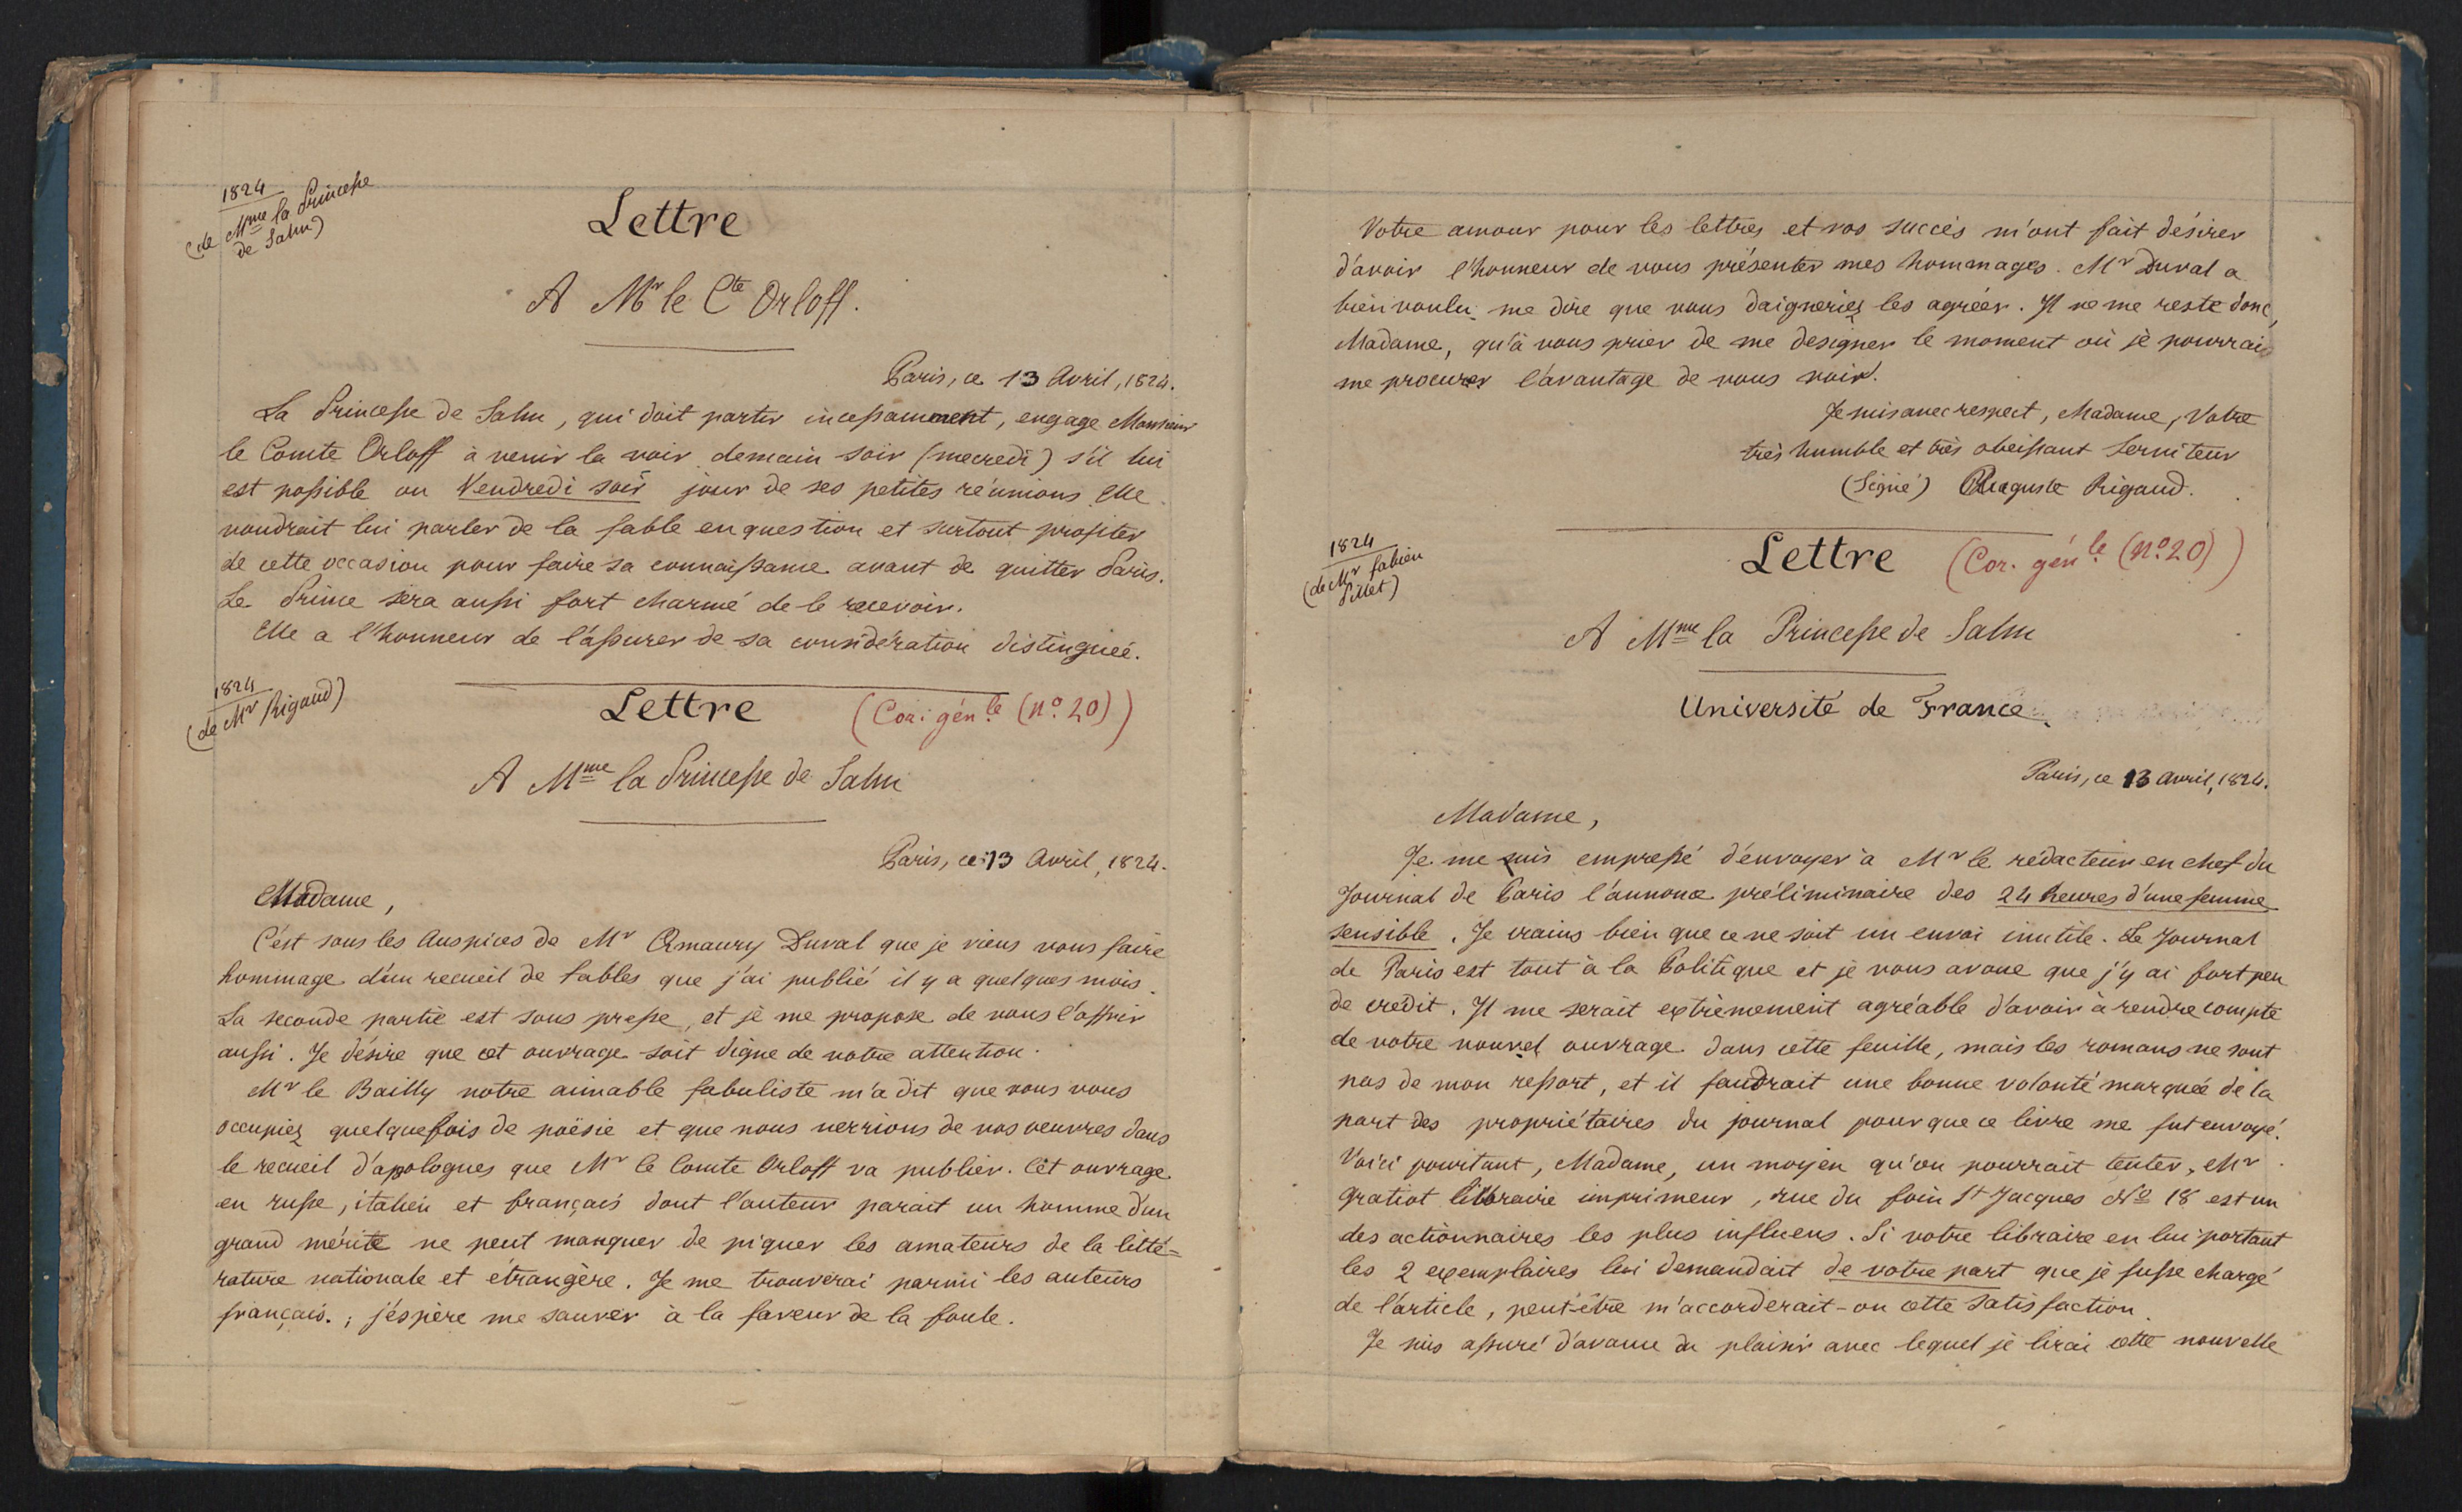
\includegraphics[width=15cm]{img/CdS02_Konv002-03_0056.jpg}
				\caption{Page présentant deux lettres puis le début de la lettre \textsf{CdS-b1-06pa} (notice \cite{CdS02056057}).}
				\label{56int}
			\end{figure}

			\begin{figure}[!h]
				\centering
				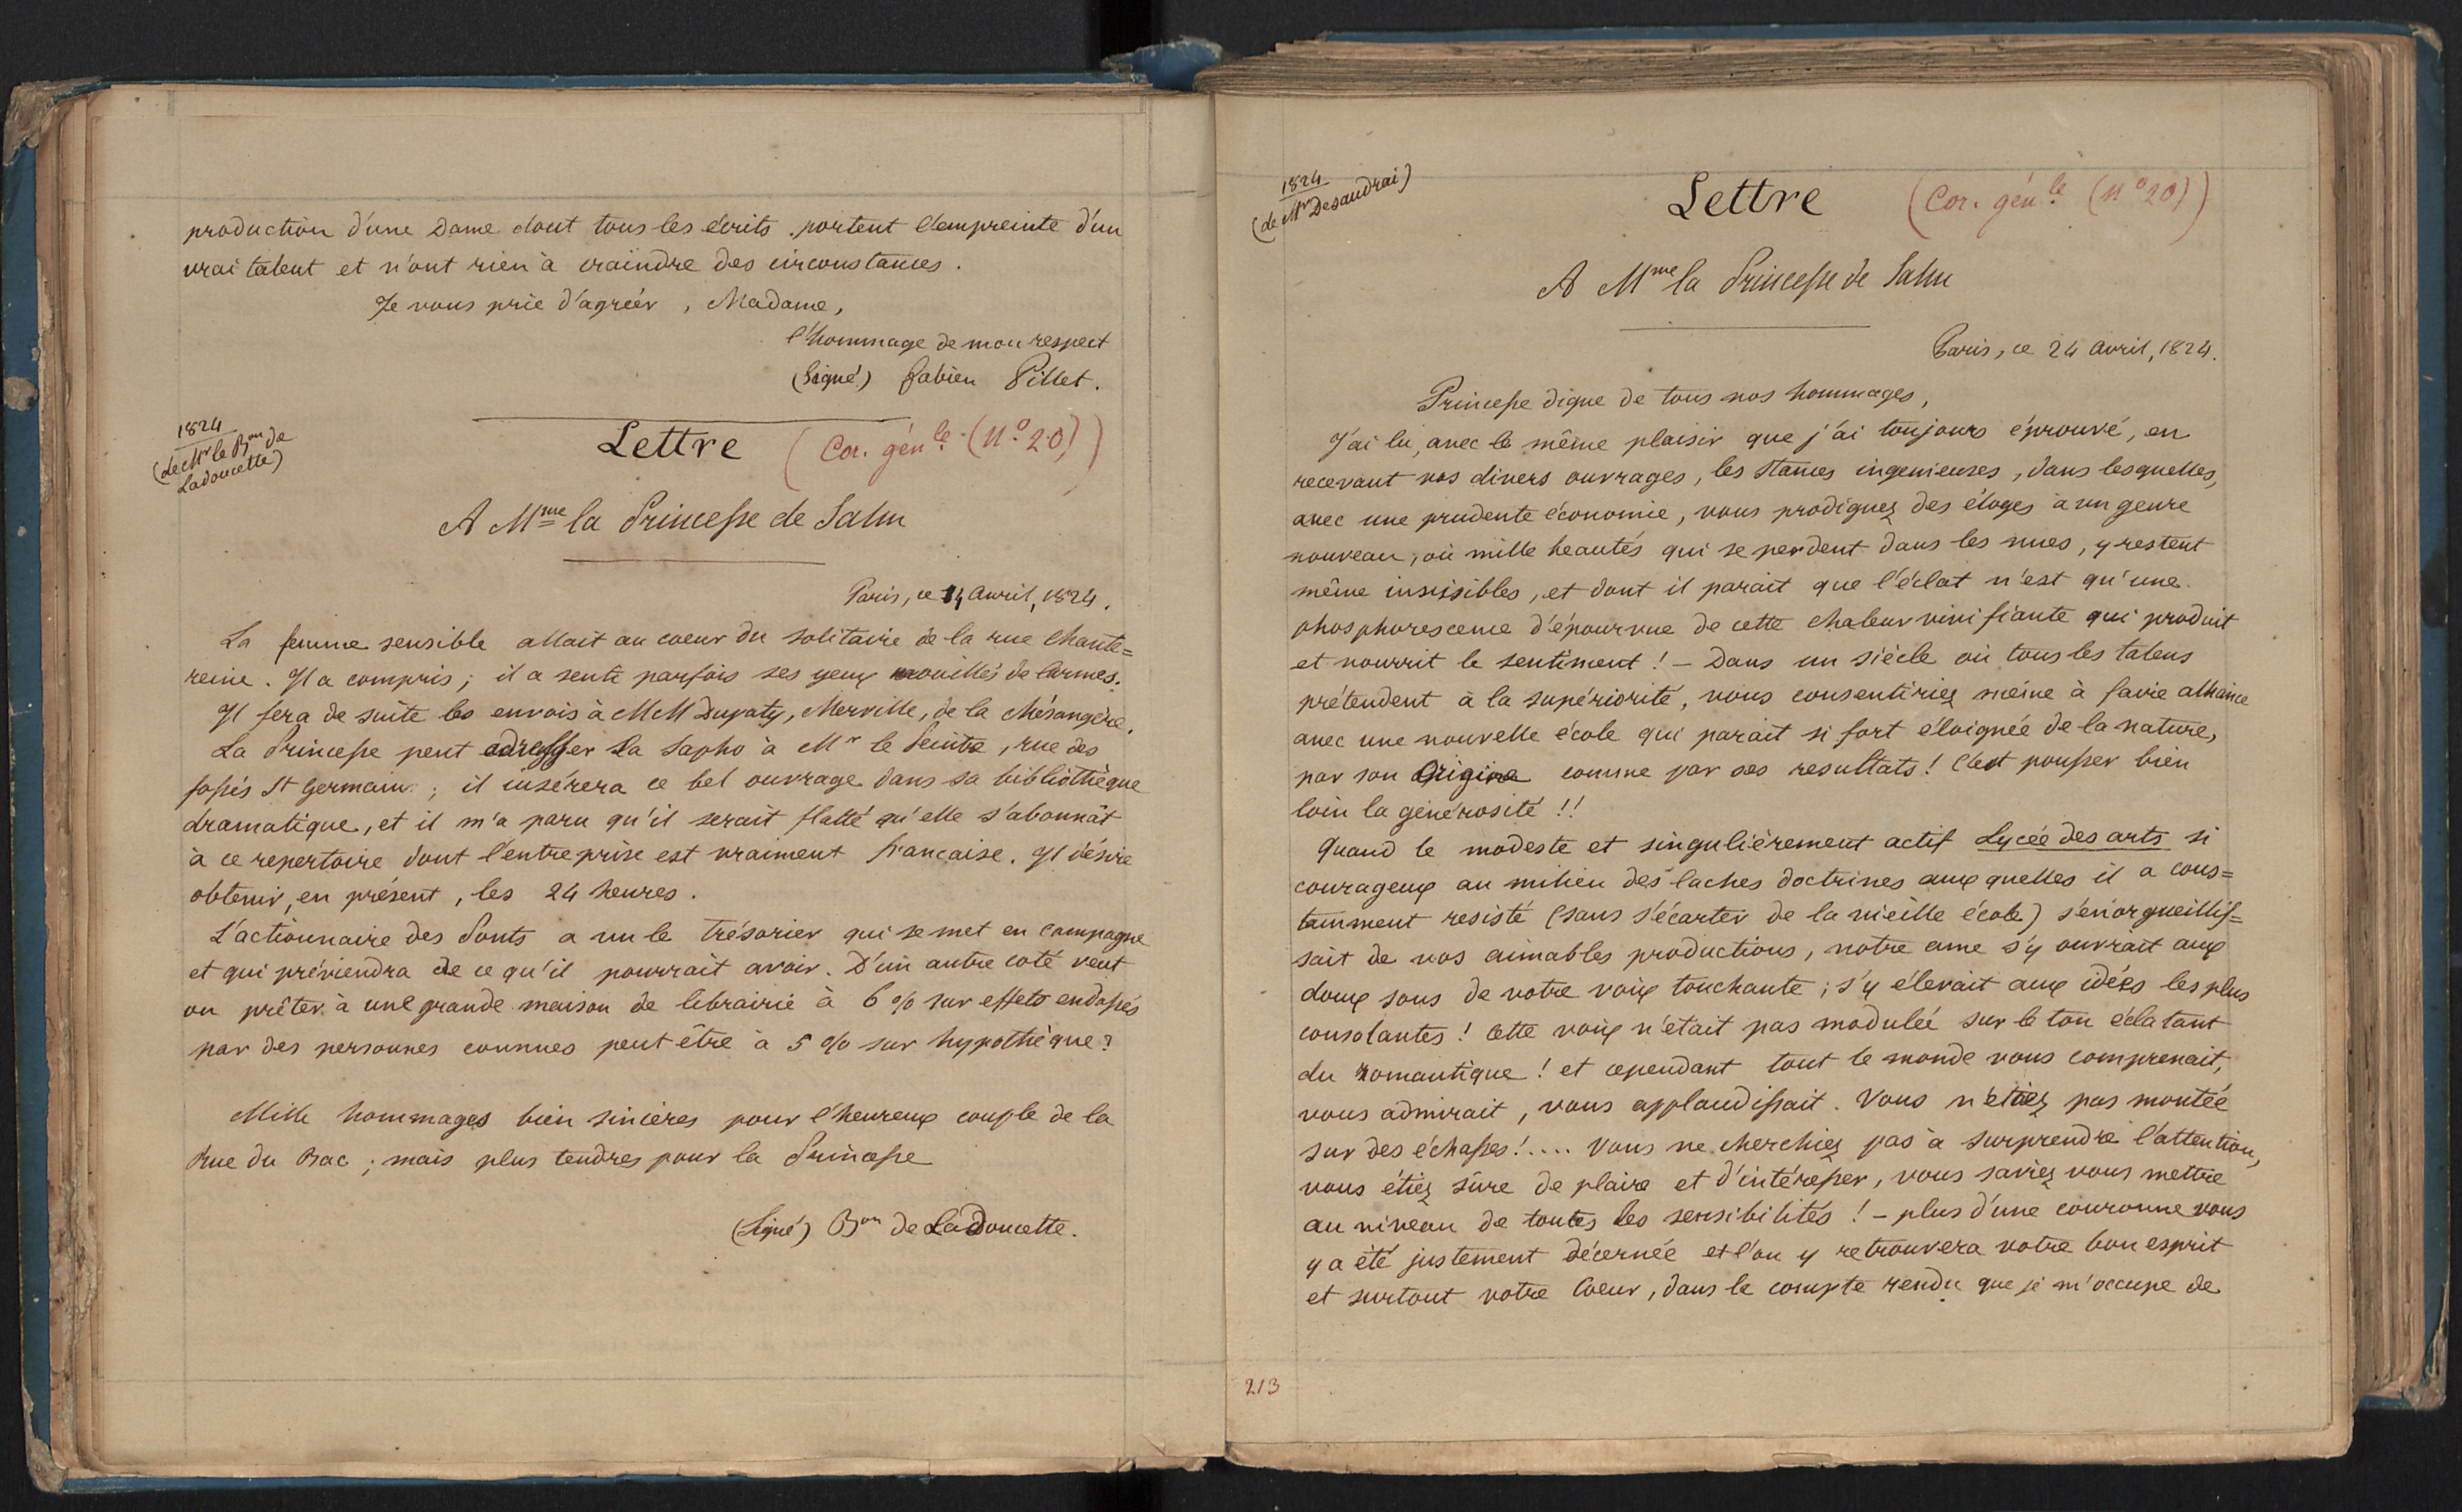
\includegraphics[width=15cm]{img/CdS02_Konv002-03_0057.jpg}
				\caption{Page présentant la fin de la lettre \textsf{CdS-b1-06pa} puis deux autres lettres.}
				\label{57int}
			\end{figure}
		
			Dans un premier temps, l'application Alto2tei importe dans l'élément \textsf{<sourceDoc>} du fichier \gls{tei} de la lettre l'intégralité du contenu des deux fichiers \gls{alto}, y compris le texte des autres lettres attestées sur les mêmes pages. Pour sélectionner le seul texte de la lettre à éditer, on s'est appuyé sur l'existence d'un titre pour chaque lettre. Ce titre a fait l'objet d'une annotation lors de la phase de {segmentation} et ses lignes sont donc accompagnées de l'information sémantique \textsf{HeadingLine:title}.
			
			Un script Python a été conçu pour intervenir dans l'application \gls{galcor} entre la construction du \textsf{<sourceDoc>} et la construction du \textsf{<text>} pour sélectionner les lignes pertinentes à éditer\footnote{Il s'agit de la fonction \textsf{selectionBlocs} dans le script \cite{biayCdsFonctionsPy2022}.}. Ce script doit récupèrer dans un premier temps une information capitale~: la position, dans la double page, du titre de la lettre à éditer. Connaissant le nombre de lettres attestées sur une même page et sachant que leurs identifiants se succèdent dans l'ordre alphanumérique, il avait été possible de calculer cette position automatiquement en générant le fichier de données dont on a montré un extrait précédemment (l'information est donnée sous la clé \textsf{title\_position})\footnote{Voir \textit{supra}, p.~\pageref{json-CdS-b1-06pa}}. On peut vérifier l'information en se reportant à l'image \ref{56int}~: le titre de la lettre d'exemple, dont le texte commence par \textit{Madame, je me suis empressé} est bien le troisième titre de la page. Le titre de la lettre ayant été localisé par sa position parmi les régions d'écriture, on procède alors à la récupération des régions d'écritures qui le suivent sur cette double page et sur la suivante, jusqu'à recontrer une nouvelle région d'écriture contenant un titre, ce qui indique qu'une nouvelle lettre est en train de commencer et que la sélection des régions pertinentes doit donc être interrompue
			\footnote{Cette opération de sélection a été effectuée au moyen de requêtes X-path construire dans le script Python grâce à la librairie Lxml (\url{https://lxml.de/}).}. Ces régions d'écritures récupérées, on en extrait la liste des identifiants de chaque ligne, car le format \gls{alto} attribue à chaque ligne un identifiant unique. C'est cette liste d'identifiant qui a permis de poser un filtre lors de la construction de l'élément \textsf{<text>} du fichier \gls{tei} à partir du contenu de son élément \textsf{<sourceDoc>}~: l'application Alto2tei a été modifiée pour ne construire l'élément \textsf{<text>} qu'à partir des lignes dont l'identifiant a été listé comme pertinent, les autres lignes étant simplement ignorées.
			
			L'extrait de données suivant montre l'information structurée (correspondant à une seule ligne de texte) à partir de laquelle est effectuée la construction du \textsf{<text>}~:
			
			\begin{minted}{js}
[
  "CdS02_Konv019_0003_z1_l16",
  "16", 
  "recommandé à tous a part de ne point inquiéter…", 
  "DefaultLine", 
  "MainZone", 
  "CdS02_Konv019_0003_z1", 
  "CdS02_Konv019_0003", 
  "eSc_line_f4af3b05"
]
			\end{minted}
			
			On constate que le texte de la ligne est transmis au script de construction accompagné de nombreuses métadonnées, sont l'identifiant unique de la ligne issu du fichier \gls{alto} (dernière donnée de la liste~: ici \textsf{eSc\_line\_f4af3b05}), ainsi que deux informations essentielles pour la suite des opérations~: le type de région d'écriture auquel la ligne appartient (ici \textsf{MainZone}) et le type de ligne lui-même (ici \textsf{DefaultLine}). Ces informations permettent en effet de structurer l'encodage de la lettre, comme on doit l'expliquer à présent.
						
		\section{Structurer l'encodage d'une lettre}

			L'opération la plus délicate de la transformation \gls{tei} est la construction de l'élément \textsf{<text>} à partir des lignes filtrées comme pertinentes. Le projet \gls{galcor} ayant vocation à transformer en \gls{tei} une très large typologie de documents, il propose une structuration très générique des textes édités. En revanche, une édition de correspondance concerne une typologie de document restreinte et implique une structuration d'encodage particulière. Ainsi le texte des lettres doit être sémantiquement structuré en trois parties principales~:
			
			\begin{enumerate}
				\item Un \textit{opener} contenant tous les éléments graphiques disposés visuellement au début de la lettre (en-tête, titre, date, nom de l'expéditeur, salutation)~;
				\item Une succession de paragraphes~;
				\item Un \textit{closer} contenant les éléments graphiques disposés visuellement en fin de lettre (salutation, signature) et qui peut éventuellement être suivi d'un post-scriptum.
			\end{enumerate}
		
			Le fait que le contenu de chaque ligne soit transmis au script de construction accompagné de ses métadonnées (et notamment des types de régions et de lignes associés au contenu) a permis d'automatiser cette structuration. Mais il fallait pour cela réécrire de manière profonde le script sur lequel l'application Alto2tei de \gls{galcor} reposait%
			\footnote{Pour le script original, voir \cite{christensenBodyBuildPy2022}~; pour son adpatation au présent proje, voir \cite{biayBuildBodyPy2022}.}.
			Cette réécriture exprime un ensemble de conditions relativement complexe, mais dont le principe général est simple~: ni le \textit{opener} ni le \textit{closer} de la lettre ne contiennent de ligne dont le type soit \textsf{DefaultLine}. Dès lors, l'énumération de chaque ligne dans l'ordre du texte permet de définir la partie dans laquelle on se situe~:
			
			\begin{enumerate}
				\item Tant que l'on ne rencontre pas de \textsf{DefaultLine}, on se situe dans le \textit{opener}~;
				\item Dès que l'on rencontre une \textsf{DefaultLine}, on se situe dans le corps de la lettre~;
				\item Dès que l'on rencontre une mention de date, une salutation ou une signature, on se situe dans le \textit{closer} (celui-ci pouvant être éventuellement suivi par un post-scriptum).
			\end{enumerate}
		
			L'arbre général des conditions de traitement des lignes est représenté par la figure \ref{cond-body}.
			
			\begin{figure}[!h]
				\centering
				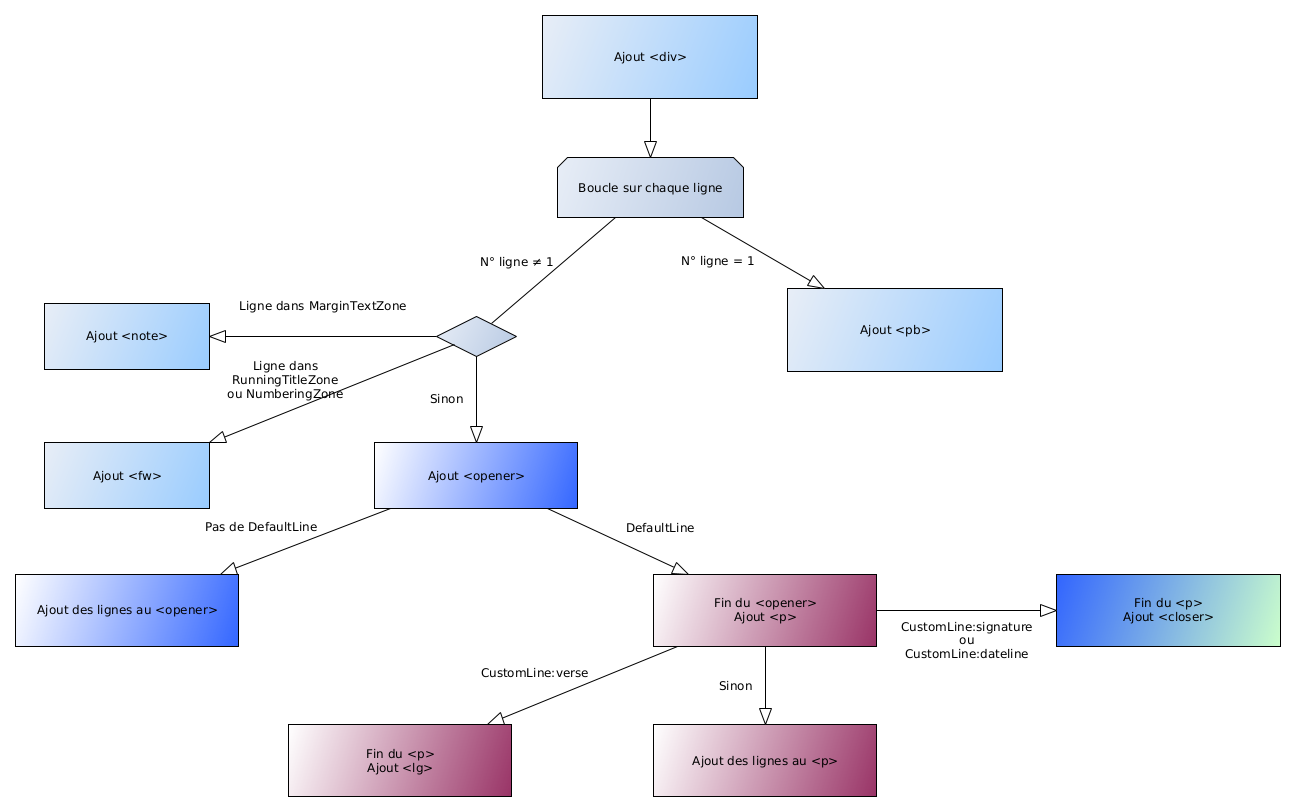
\includegraphics[width=15cm]{schema/build-body.png}
				\caption{Arbre des conditions de traitements des lignes pour la construction de l'édition (image en haute définition disponible \href{https://raw.githubusercontent.com/sbiay/CdS-edition/main/rapportBiay/schema/build-body.svg}{ici}).}
				\label{cond-body}
			\end{figure}
		
			Outre les principales parties du texte, il fallait tenir compte des éléments marginaux~: systèmes de numérotation (page, lettre), notes, annotations érudites ou d'origine, titres courants. Il n'était pas possible d'associer strictement ces éléments à leur lettre. Lorsque plusieurs pages se partagent la même lettre, la numérotation des éléments marginaux ne s'inscrit pas toujours au bon endroit dans la succession des régions d'écriture (ces éléments sont souvent rejetés en fin de numérotation). Pour que ce problème ne passe pas inaperçu, l'encodage automatique attire l'attention de l'éditeur de la façon suivante~:
			
			\begin{minted}{xml}
<note type="MarginTextZone">
  <!--Vérifier que la note corresponde à la lettre et mettre à jour le type-->
  [transcription de la note]
</note>
			\end{minted}
		
			Une dimension importante de la complexité de l'encodage des lettres a été l'alternance présentée par certaines entre contenu prosaïque (à transformer en éléments \textsf{<p>}) et contenu versifié (à transformer en élément \textsf{lg}). Encore une fois, l'annotation des lignes permet de les traiter de la manière adéquate (\textsf{CustomLine:verse} dans le cas des parties versifiées). 
			
			On présente ici à titre d'exemple le résultat de l'encodage automatique d'un texte singulier dans sa constitution, car il contient un poème en tant que post-scriptum.
			
			\begin{figure}[!h]
				\centering
				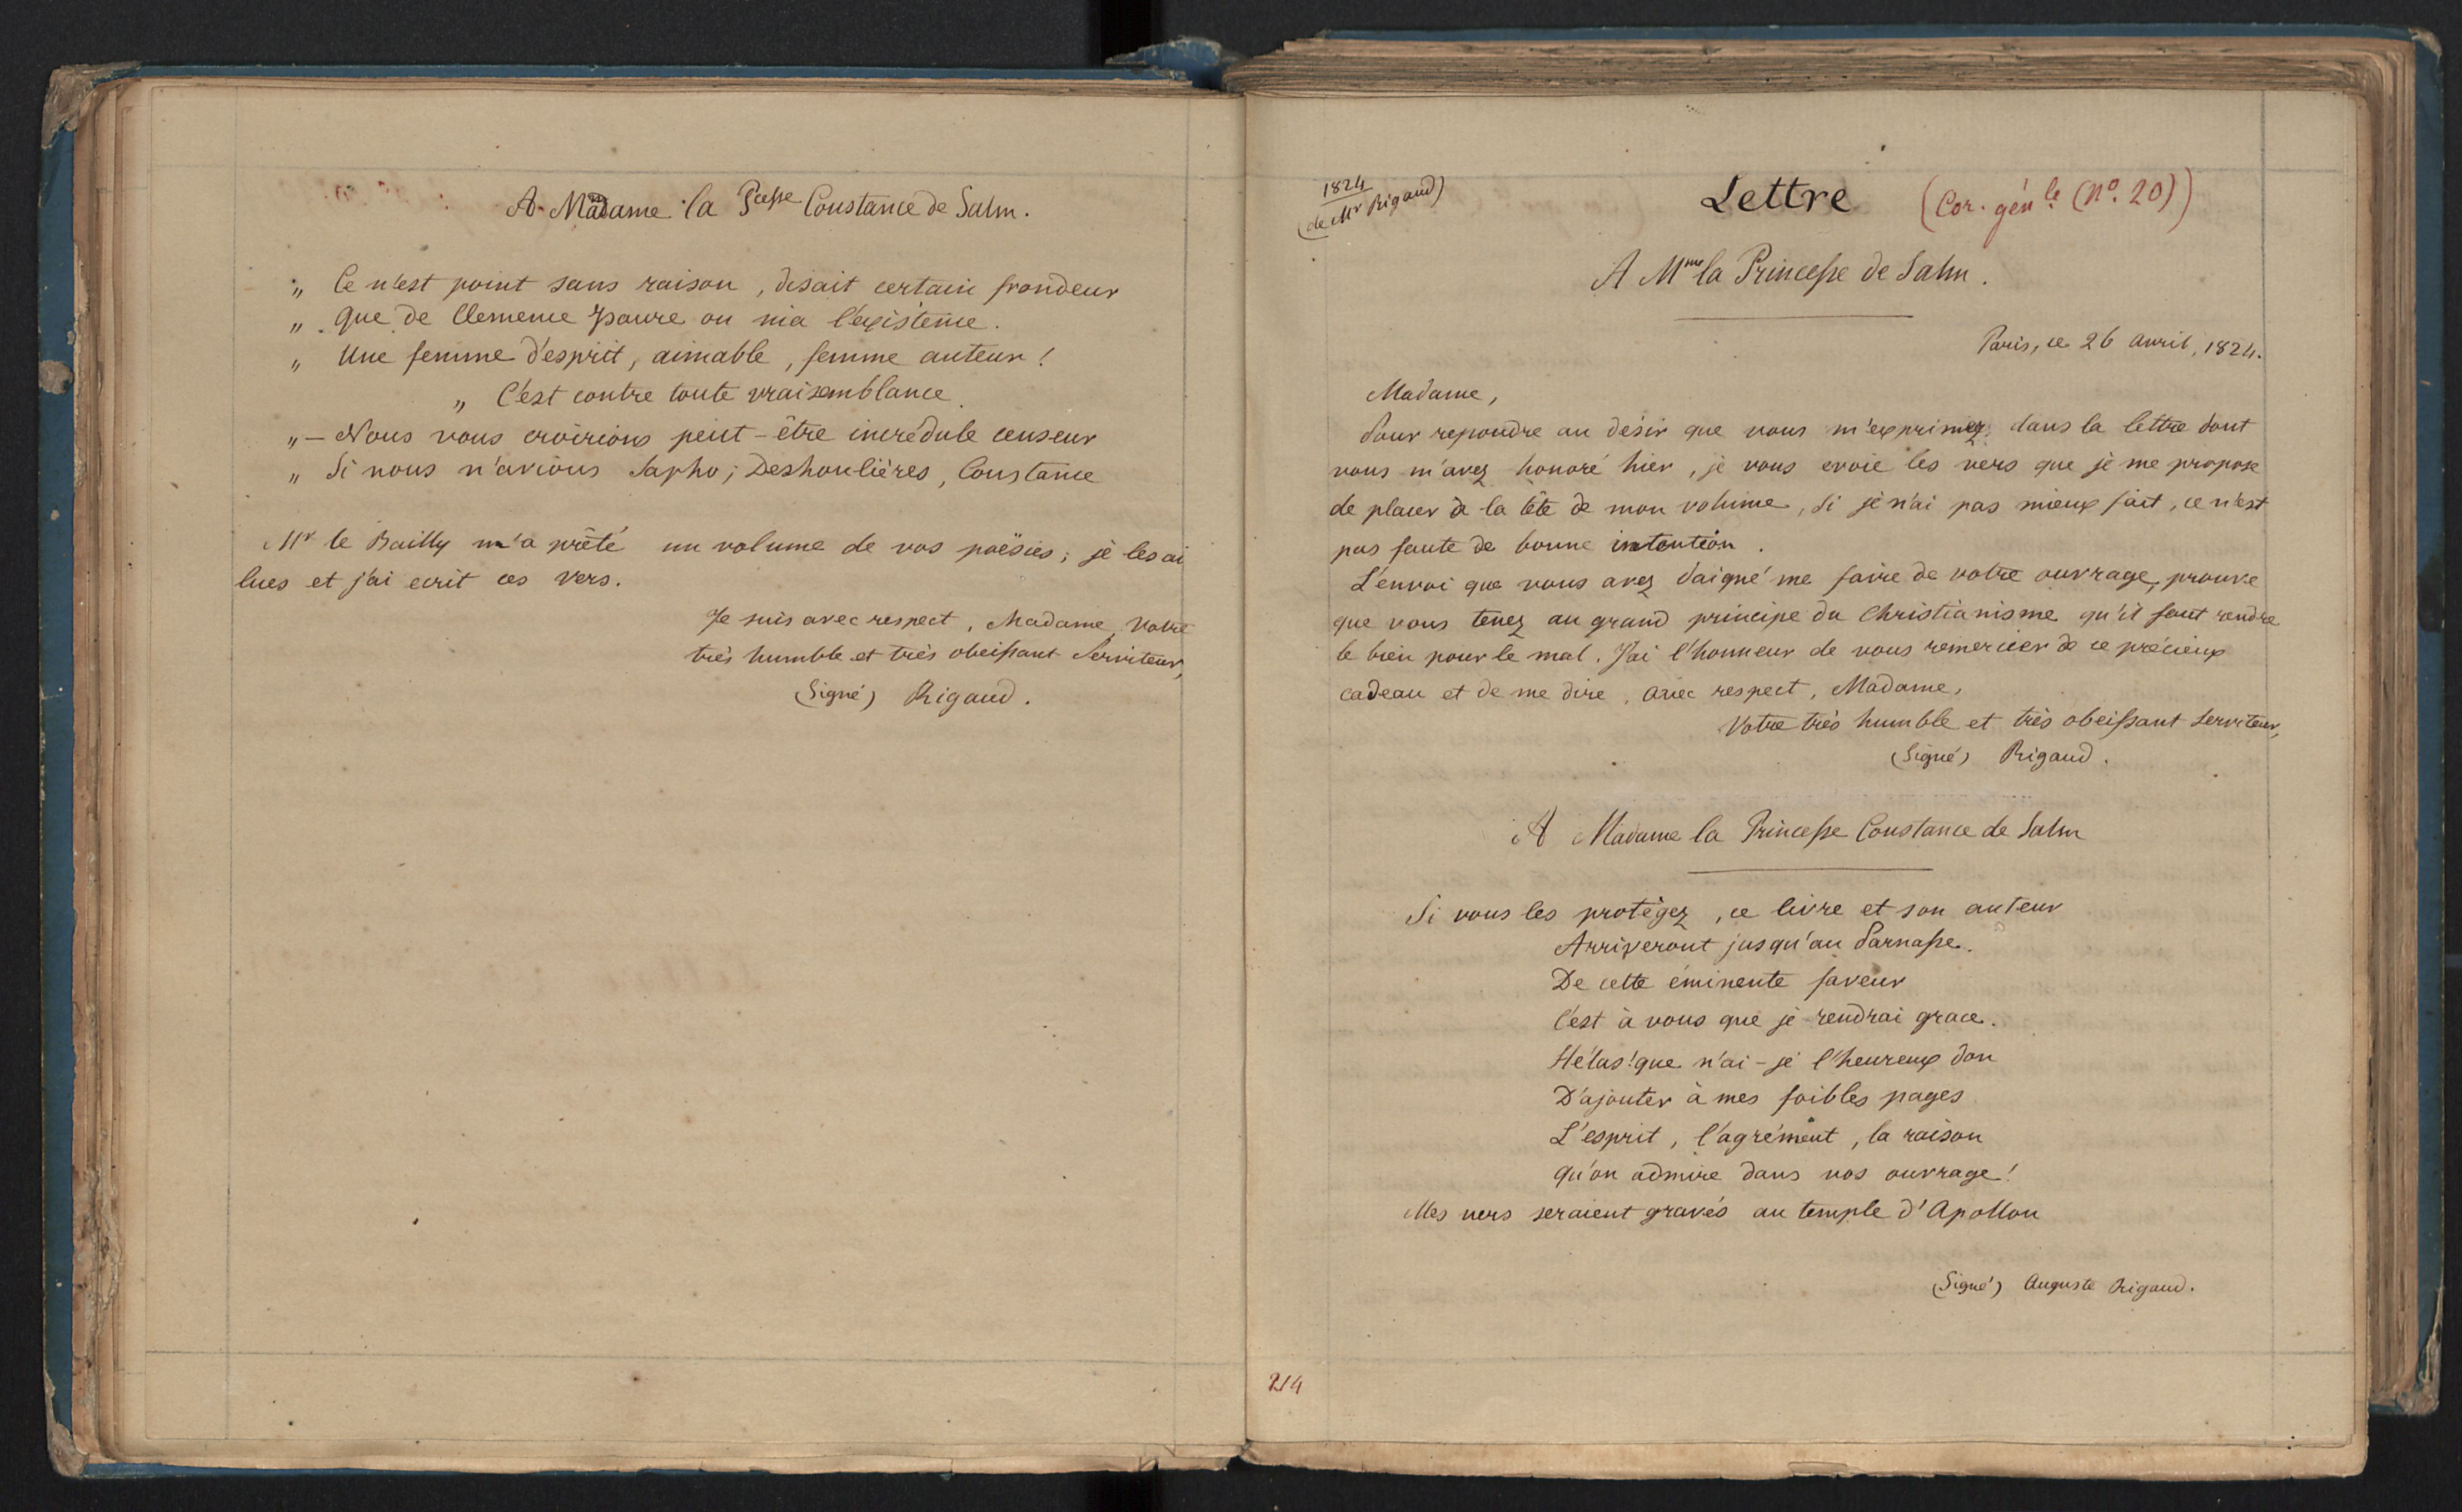
\includegraphics[width=15cm]{img/CdS02_Konv002-03_0059.jpg}
				\caption{Lettre de P.-A.~Rigaud à \gls{cds} (notice \cite{CdS02059})).}
				\label{}
			\end{figure}
			
			\small
			
			\begin{minted}{xml}
<div>
  <opener>
    <fw type="letterhead"><lb/>1824<lb/>(de Mr Rigaud)</fw>
    <title><lb/>Lettre<lb/>A Mme la Princesse de Salm.</title>
    <note><lb/>(Cor. génle. (n° 20)</note>
    <dateline><lb/>Paris, ce 26 avril, 1824.</dateline>
    <salute><lb/>Madame,</salute>
  </opener>
  <p><lb/>vous m'avez honoré hier, je vous evoie les vers que je me propose
    <lb/>Pour repondre au désir que vous m'exprimez, dans la lettre dont<lb/>
    de placer de la tête de mon volume, Si je n'ai pas mieux fait, ce n'est
    <lb/>pas faute de bonne intention.<lb/>L'envoi que vous avez daigné me 
    faire de votre ouvrage, prouve<lb/>que vous tenez au grand principe du 
    Christianisme qu'il faut rendre<lb/>le bien pour le mal. J'ai l'honneur 
    de vous remercier de ce précieux<lb/>cadeau et de me dire, avec respect, 
    Madame,
  </p>
  <closer>
    <signed><lb/>Votre très humble et très obéissant Serviteur,
    <lb/>(Signé) Rigaud.</signed>
  </closer>
  <postscript>
    <p><lb/>A Madame la Princesse Constance de Salm</p>
    <lg>
      <l><lb/>Si vous les protègez, ce livre et son auteur</l>
      <l>Arriveront jusqu'au Parnasse.</l>
      <l><lb/>De cette éminente faveur</l>
      <l><lb/>C'est à vous que je rendrai grace.</l>
      <l><lb/>Hélas ! que n'ai-je l'heureux don</l>
      <l><lb/>D'ajouter à mes faibles pages</l>
      <l><lb/>L'esprit, l'agrément, la raison</l>
      <l><lb/>Qu'on admire dans vos ouvrage !</l>
      <l><lb/>Mes vers seraient gravés au temple d'Apollon</l>
    </lg>
    <signed><lb/>(Signé) Auguste Rigaud.<!--Salut--></signed>
  </postscript>
  <fw corresp="#CdS02_Konv002-03_0059_z4" type="NumberingZone">
    <lb/>214<!--Vérifier que le numéro corresponde à la lettre et 
    mettre à jour le type : pageNum ou letterNum -->
  </fw>
</div>

			\end{minted}
		
			\normalsize
			Enfin, les corrections écrites dans l'interligne ont elles aussi été annotées de façon particulière (\textsf{InterlinearLine}), ce qui permet de les traiter dans un encodage qui exprime leur fonction de correction du texte original.
			
			\begin{figure}[!h]
				\centering
				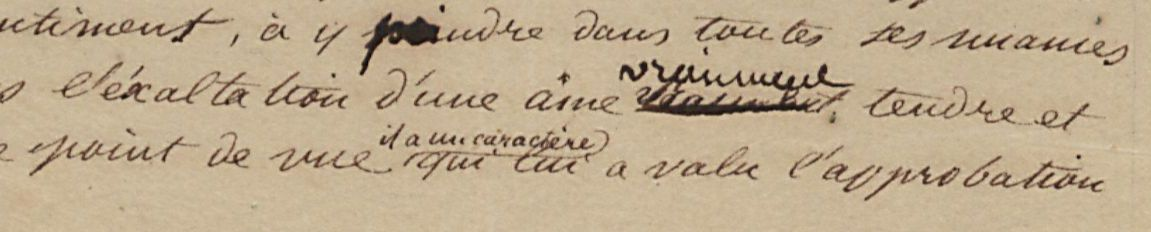
\includegraphics[width=15cm]{img/CdS02_Konv002-03_0072-detail-corr.jpg}
				\caption{Exemple de correction interlinéaire (notice \cite{CdS02072}).}
				\label{}
			\end{figure}
		
			L'encodage automatique prend la forme suivante (les balises de début de ligne ont été supprimées pour davantage de clarté)~:
			
			\begin{minted}{xml}
l'éxaltation d'une âme [........] tendre et
<!--Correction interlinéaire-->
<choice>
  <sic/><!--Partie laissée vide car non prédictible par le script-->
  <corr>
    vraiment
  </corr>
</choice>
			\end{minted}
			
			Bien entendu, cet encodage ne constitue qu'une étape intermédiaire, laissant une partie de travail non automatisable à la responsabilité de l'éditeur, qui en l'occurrence doit préciser que la partie corrigée n'est pas lisible~:
			
			\begin{minted}{xml}
l'éxaltation d'une âme 
<choice>
  <sic>
    <unclear reason="illegible"/>
  </sic>
  <corr>
    vraiment
  </corr>
</choice> tendre et
			\end{minted}
		
			Le bon fonctionnement des scripts d'encodage a été testé sur une sélection de lettres, choisies pour la diversité des cas de figures qu'elles présentaient\footnote{La collection de test se trouve à l'adresse suivante~: \url{https://github.com/sbiay/CdS-edition/tree/main/transformation-alto-tei/collection-test}.}. Il s'agissait de structurer correctement des lettres se développant sur plusieurs pages (sur deux pages ou sur plus de deux pages), mais aussi de bien distinguer plusieurs lettres écrites sur la même page, cas particulièrement fréquent dans les recueils de copies. L'automatisation de l'encodage a été testée tout particulièrement avec ces recueils de copies, documents très structurés, comportant des manchettes, des notes infrapaginales, des corrections, des textes en vers, et où les lettres se succèdent sans laisser de blanc. Il va de soi que la bonne structuration de l'encodage de ces documents complexes garantit la bonne structuration des documents plus simples. 
			
			Dans l'éventualité où une lettre serait dépourvue de titre, élément-clé de la méthode d'encodage que l'on a élaborée, la production de l'édition ne serait pas pour autant rendue impossible~: le contenu du texte serait encodé malgré tout, avec le texte des documents qui le précèdent ou qui le suivent sur la même page, obligeant à la suppression manuelle de ces parties.
			
		\section{Inscrire les métadonnées dans l'en-tête de la lettre}
		
			\subsection{Décrire la lettre}
				Le projet \gls{galcor} ne traitant que des sources publiées sur Gallica, il récupère les métadonnées bibliographiques dans deux sources principales~: les manifestes 3IF\footnote{Il s'agit de fichiers au format \gls{json}. Pour un bref aperçu des principes de ce mode d'exposition des données, voir \cite{robineauComprendreIIIFInteroperabilite2016}.} des documents et le catalogue général de la \gls{bnf}.
				
				Les métadonnées de la correspondance de \gls{cds} ont quant à elle été publiées sur la plateforme Zenodo dans un format tabulaire\footcite{peyronnetdrydenInventarKorrespondenzConstance2021}. Il est donc aisé d'associer le fichier \gls{tei} à ses métadonnées en allant chercher dans ces tableaux l'identifiant de la lettre à éditer. Le script \textsf{build\_teiheader} de l'application Alto2tei a été modifié pour procéder à cette récupération inscrire des données choisies dans l'arborescence de l'en-tête du fichier \gls{tei}. L'inscription de ces données a lieu au niveau de l'élément \textsf{<profileDesc>}, au sein d'un sous-élément spécialement dévolu à la description des correspondances~: le \textsf{<correspDesc>}. Celui-ci comporte des éléments obligatoires (\textsf{<correspAction>}) pour la description de l'expédition (expéditeur, lieu, date) et de la réception d'une lettre.
				
				\small
				\begin{minted}{xml}
<profileDesc>
  <correspDesc>
    <correspAction type="sent">
      <persName ref="https://viaf.org/viaf/121051">
        Salm, Constance de (CdS)
      </persName>
      <placeName ref="https://www.geonames.org/2894637">
        Dyck (Schloss), Gde. Jüchen
      </placeName>
      <date when-iso="1816-01-14">1816-01-14</date>
    </correspAction>
    <correspAction type="received">
      <persName ref="n/a">Prous, Henry</persName>
    </correspAction>
  </correspDesc>
</profileDesc>
				\end{minted}
				\normalsize
			
				Il convient également de donner une expression plus littéraire à ces données. C'est le rôle de l'élément titre (\textsf{<title>}) du document \gls{tei} que l'on a forgé de manière automatique, par la manipulation des chaînes de caractères du nom de l'expéditeur, du destinataire, du lieu et de la date d'expédition (avec les mentions s.l. et s.d. dans le cas de lettres sans lieu ou sans date). Il s'agissait notamment de simplifier les noms (débarassés des titres de noblesse) et de rétablir le prénom avant le patronyme, ou encore d'exprimer la date en toutes lettres. Toujours pour la même lettre (et donc à partir des mêmes données brutes), le titre a été exprimé de la façon suivante~:
				
				\small
				\begin{minted}{xml}
<title>
  Lettre de Constance de Salm à Henry Prous (Dyck, le 14 janvier 1816)
</title>
				\end{minted}
				\normalsize
				
				
			\subsection{Citer la notice de l'inventaire}
			
				Il était également essentiel d'inscrire dans l'en-tête du fichier \gls{tei} la référence bibliographique de la notice de la lettre publiée en ligne. Cette description intervient dans l'élément \textsf{<sourceDesc>}~:
				
				\small
				\begin{minted}{xml}
<sourceDesc>
  <biblStruct>
    <analytic>
      <title>CdS/19/002</title>
      <idno>https://constance-de-salm.de/archiv/#/document/10462</idno>
    </analytic>
    <monogr>
      <title>
        La correspondance de Constance de Salm (1767-1845). 
        Inventaire du fonds Salm de la Société des Amis du Vieux Toulon et de sa Région 
        et du fonds Constance de Salm, Archiv Schloss Dyck (Mitgliedsarchiv 
        der Vereinigten Adelsarchive im Rheinland e.V.). Édition numérique
      </title>
      <imprint>
        <publisher>DHI Paris</publisher>
        <pubPlace>Paris</pubPlace>
        <date>2021</date>
      </imprint>
    </monogr>
  </biblStruct>
</sourceDesc>
				\end{minted}
				\normalsize
				
			\subsection{Renseigner les données du projet}
			
				Enfin, les données descriptives du projet, l'édition de la correspondance dans son ensemble, ont été décrites dans l'élément \textsf{<seriesStmt>} de la façon suivante (l'encodage des noms a été simplifié)~:
				
				\small
				\begin{minted}{xml}
<seriesStmt>
  <title>La correspondance de Constance de Salm (1767-1845)</title>
  <respStmt>
    <resp>Encadrement scientifique et technique du projet</resp>
    <persName>Anne Baillot</persName>
    <persName>Mareike König</persName>
    <persName>Floriane Chiffoleau</persName>
  </respStmt>
  <respStmt>
    <resp>Réalisation de la chaîne de traitement</resp>
    <persName>Sébastien Biay</persName>
  </respStmt>
</seriesStmt>
				\end{minted}
				\normalsize

		\section{Finaliser l'encodage d'une lettre}
		
			Un certain nombre de tâches non automatisables ont fait l'objet d'une documentation fonctionnelle, exemples à l'appui\footcite{biayFinaliserEncodageLettre2022}.
			
			La première consiste à diviser les paragraphes. En effet, les zones d'écriture définies au moment de la \gls{segmentation} engloble les paragraphes d'une manière indistincte, et seul l'oeil humain permet de resconstituer cette structure à posteriori.
			
			Les corrections interlinéaires, en partie encodées automatiquement, doivent être réinsérées dans la ligne où se trouve la partie corrigée. On l'a également dit plus haut~: les notes marginales et éléments de numérotation doivent être contrôlées et parfois déplacées.
			
			Il n'a pas été prévu de script pour la résolution automatique des abréviations courantes, ce qui aurait été possible avec davantage de temps bien entendu. 
			
			D'une manière générale, l'édition numérique de la correspondance de \gls{cds}, avec les subtilités d'encodage inhérentes à ce type de travail, comme la création d'un apparat critique pour corriger le texte là où le copiste a commis des fautes manifestes, ne peut pas se satisfaire d'une simple documentation fonctionnelle. L'enjeu appelle la rédaction d'un schéma \gls{odd} qui établisse de manière précise et exhaustive les règles d'encodage de la correspondance et en porte la spécification technique\footnote{Une ODD joue à la fois un rôle de documentation pour les contributeurs du projet, sorte de guide d'encodage, et de validation technique des documents.}. Sa mise en œuvre étant un travail exigeant, les dimensions du stage ne permettaient pas d'atteindre cet objectif supplémentaire\footnote{On s'est contenté de finaliser manuellement l'encodage de trois petites lettres, afin de pouvoir en évaluer les possibilités d'exploitation. Cf.~\url{https://github.com/sbiay/CdS-edition/tree/main/transformation-alto-tei/final}}.
			
	\chapter*{Conclusion}
		\addcontentsline{toc}{chapter}{Conclusion}% Ajoute à la table des matières sans numérotation
		
		La correspondance de \gls{cds} est un vaste corpus (11\,000 pièces environ), constitué de documents de nature hétérogène (originaux, brouillons, copie), en feuilles libres ou constitués en recueils, copiés par de multiples mains. Il n'était guère possible d'analyser de manière complète ces documents, que ce soit sur le plan de la mise en page, sur le plan paléographique ou sur le plan de la conservation, et cette absence d'une évaluation globale est une limite évidente aux apports de ce stage. Mais, s'il eut été trop coûteux de dresser la cartographie complète du territoire, le front pionnier que l'on y a ouvert en facilitera sans doute l'exploration de manière considérable.
		
		On s'est ainsi attelé à trois problèmes inhérents à toute entreprise d'édition nativement numérique d'un corpus massif~: 
		
		\begin{enumerate}
			\item Analyser la mise en page des documents (par l'entraînement d'un modèle de segmentation des pages)~;
			\item Produire un modèle capable de reconnaître simultanément les écritures de plusieurs copistes et rendre sa méthode d'entraînement réitérable~;
			\item Structurer l'édition lettre par lettre à partir de sources où elles ont été copiées ensemble, et ce de manière automatisée.
		\end{enumerate}
		
		Pour relever ces différents défis, il fallait déterminer à quel endroit ouvrir le front. On s'est principalement attaché aux documents qui sont apparus comme les plus complexes, à savoir les recueils de la seconde copie\footnote{\cite{CdS02001330}~; \cite{CdS02001369}~; \cite{CdS02001334}.}~:
		
		\begin{enumerate}
			\item Ce sont les documents présentant la mise en page la plus structurée (titres, manchettes)~;
			\item Les éléments marginaux y sont nombreux (systèmes de classement par type de lettre, numérotation des pages, notes érudites)~;
			\item Elles contiennent de nombreux documents non inventoriés~: il était donc nécessaire de trier les documents à éditer et les documents à écarter.
		\end{enumerate}
		
		Aborder les documents apparaissant comme les plus complexes permet de penser que la chaîne de traitement qui a été mise en place est dotée d'une vraie robustesse, et qu'elle permettra sans mal de traiter des documents plus simples. 
		
		Au demeurant, toutes les difficultés de traitement des documents n'ont pas pu être prises en compte. On a notamment identifié un problème de transparence du papier dans la correspondance de J.-P.~Martini à \gls{cds}, qui mériterait de réfléchir à une méthode de pré-traitement des images\footnote{Voir par exemple la lettre \cite{CdS19054056}.}.
		
		L'analyse de la mise en page, par l'entraînement d'un modèle de \gls{segmentation}, n'a produit que des résultats partiels, mais encourageants. Les méthode d'entraînement sont amenées à évoluer rapidement dans les années à venir et l'on peut penser que l'approche de la \gls{segmentation} que l'on a envisagée sera rapidement dépassée. Mais cette approche a néanmoins abouti à un gain de temps réel dans le traitement des pages, seules les petites subtilités comme les mentions de date, les signatures, etc. représentant un réel problème. Malgré cet inaboutissement, il était important de ne pas sacrifier trop de temps à cette étape du travail afin de mettre en place une chaîne de traitement relativement complète, qui aboutisse à la construction de l'édition numérique au format \gls{tei}.
		
		L'entraînement d'algorithmes de reconnaissance des écritures manuscrites a en revanche rencontré moins de difficultés. Grâce aux apports méthodologiques et aux modèles récupérés du projet \gls{lectaurep}, d'excellents scores ont pu être obtenus avec relativement peu de données d'entraînements produites.
		Il a un temps été envisagé d'entraîner un modèle pour reconnaître l'écriture autographe de \gls{cds}, mais la transcription de ses brouillons s'est révélée gourmande en temps, avec le risque que le résultats se révèlent mauvais. On s'est donc contenté de donner en annexe les transcriptions effectuées afin de faciliter le travail d'un futur paléographe.
		La méthodologie de correction semi-automatisée qui a été inspirée par le projet \gls{dahn} a également été approfondie et élaborée pour parvenir à des résultats très satisfaisants en termes de fonctionnalité. Mais l'on conserve un doute sur l'utilité de ce dispositif dans le contexte d'une édition, où la relecture du texte est toujours nécessaire au moment de la réalisation de l'encodage final. Dissocier (pour l'automatiser) une partie de la correction de texte de cette phase finale est-elle vraiment rentable~? La réponse peut certes dépendre des conditions dans lesquelles est mené le projet, ce sur quoi l'on reviendra dans un instant.
		
		Enfin, l'on a abordé dans les dernières semaines (pour ne pas dire dans les derniers jours) du stage la phase de transformation des transcriptions automatiques en édition au format \gls{tei}. L'application Alto2tei du projet \gls{galcor} a permis un gain de temps considérable. La production d'éditions structurées a ainsi pu être menée à bien, mais le volet philologique du travail demeure incomplet, en l'absence d'une \gls{odd} en bonne et due forme, dont le \textit{Guide d'encodage pour l'édition numérique des égo-documents} du projet \gls{dahn} devrait constituer la meilleure matrice possible\footcite{chiffoleauGuideEncodagePour2022}. L'encodage pourrait en outre être poussé plus loin qu'on ne l'a fait, avec la reconnaissance des entités nommées (processus automatisable) ou la description des mains intervenant sur chaque lettre (copiste, corrections souvent effectuées par \gls{cds}, érudit).
		
		La chaîne de traitement que l'on a produite devrait permettre de mener efficacement l'édition numérique de la correspondance de \gls{cds} sans requérir d'importantes compétences en ingénierie ou en langages de programmation. Mais il est illusoire de penser qu'elle puisse parfaitement fonctionner pour tous les documents du corpus et que l'on puisse se l'approprier sans une bonne connaissance du XML (et de la TEI en particulier) ainsi que des notions de langage Python et d'utilisation d'un système d'exploitation Linux%
		\footnote{On a pu tester le fonctionnement de l'application Kraken dans une machine virtuelle sous Windows, mais pas l'installation complète de la chaîne de traitement.}. %
		La phase la plus délicate de la prise en main sera nécessairement son installation. Mais, alors qu'il nous a fallu déployer l'interface eScriptorium localement (ce qui n'a pas été simple), l'ouverture prochaine d'une instance de cette application hébergée par Paris Sciences et Lettres devrait grandement simplifier son l'accès à cet outil essentiel. 	
		Passées les difficultés du démarrage, les phases les plus chronophages du travail éditorial resteront la correction de la \gls{segmentation} des pages, la production de vérités de terrain ou la correction des \glspl{prédiction}, ainsi que la finalisation de l'encodage, dont une liste de tâches demeurent impossibles à automatiser.
		
		Il pourrait être intéressant, pour le développement futur du projet, d'engager un nouveau chantier d'ingénierie pour créer une plateforme de transcription collaborative, où la prédiction brute des textes serait proposée à la correction par les contributeurs, accélérant ainsi la constitution de vérités de terrain ou la correction préalable à l'encodage en \gls{tei}… 
		
		La route vers une édition complète de la correspondance de \gls{cds} sera longue quoiqu'il arrive, et nous n'avons fait qu'atteindre un premier relais. Mais l'histoire des femmes de lettres suscite l'adhésion du public et des institutions, et l'adéquation entre l'\og honnête liberté \fg \footcite{CdS02045046} louée par \gls{cds} et l'esprit du temps pourrait placer ce projet éditorial sous des auspices favorables.
		
		%ICI
			
				
	\appendix
	
	\renewcommand{\appendixpagename}{Annexes}
	% Pour renommer en "Annexes" la page de titre "Appendices"
	
	\renewcommand{\appendixtocname}{Annexes}
	% Pour renommer en "Annexes" le nom des annexes dans la table des matières
	
	\addappheadtotoc% Ajoute les annexes à la table des matières
	
	\appendixpage % Crée une page de titre pour les annexes
	
	\chapter{Transcriptions \\de deux manuscrits autographes \\de C.~de Salm}
		\label{autographes}
		
		\section{Premier extrait}
	
			La ponctuation a été quelque peu modernisée pour rejoindre une édition de type diplomatique.
		
			Extrait du début de la lettre de C.~de Salm à Therese Thurn und Taxis du 20 mai 1825\footcite{CdS67022030}~:
			
			\begin{quotation}
				\begin{flushright}
					Dyck, ce 20 mai 1825.
				\end{flushright}
				
				\begin{center}
					Madame,
				\end{center}
	
				Que vous dire de mon silence ?
				
				Comment pourrai-je l'expliquer ?
				
				je n'en sais rien~: le travail, la soufrance
				
				le repos ; est ennui qui vient tout attaquer,
				
				fruit de longues douleurs, dont la premiere me
				
				semble ††††ante pour jamais
				
				le charme d'une douce et simple jouissance,
				
				voilà pourquoi, si j'en crois l'apparence,
				
				depuis si longtemps me tais.
				
				Cependant, je dois vous le dire,
				
				moi mème je ne puis bien décider ce point ;
				
				car si je ne vous écris point,
				
				à chaque instant, je voudrais vous écrire.
				
				Mais le Printems, son éclat, sa fraicheur,
				
				La nature si belle en ses jours des pleud†††
				
				par leur vivifiante flamme
				
				de mon Corps épuisé raniment les ressorts.
				
				Ces jeunes fils, vrai soutiens de mon âme
				
				Sans le savoir secondant ses efforts
				
				de l'existance, aussi, me rouvrent les trésors
				
				et charmeur de nouveau narcoi†
				
				par luy de grands chaos d'esperances remplis.
				
				Enfin le sort et plus juste et plus doux
				
				pour un moment au moins de mes maux me soulage
				
				je sens renaitre en moi le calme, le courage
				
				je me retrouve et je reviens à vous.
							
				Voici, Madame le tableau fidele de tout ce qui
				passe en moi depuis que je ne vous ai ecrit, et de
				tout ce que j'éprouve aujourdhui. Mon ††††† en est fort
				triste. Ce n'est pas mon absence de Paris qui en est cause :
				Mon âge ; mes habitudes de travail ne me permettent pas
				de†††† cet' privation si vivement, C'est cet' vieille
				douleur qui est toujours ici, et aussi la perte d'une
				foule de mes amis et de personnes, de connaissance.
				Encore tout recemment j'ai vu disparaitre Derrou,
				la P(rin)cesse Borghese avec qui j'avais été tres liée, et qui
				etait une aimable personne, et le malchanceux courrier, assassiné
				près de son chateau, dieu sait par qui ! ‒ (vous auriez vu ce malheur
				dans les journaux). Ce que l'on dit sur les causes de ce terrible
				èvènement est affreux † pa††r, et je n'ose l'écrire. […]			
			\end{quotation}
	
		\clearpage
		\section{Second extrait}
			\label{trans-C11S92047049}
			Extrait du début de la lettre de C.~de Salm à Fürst von Hatzfeldt du 2 mars 1828\footcite{C11S92047049}~:
			
			\begin{quotation}
				\begin{flushright}
					Dyck ce 2 Mars 1818.
				\end{flushright}
				
				Vous serez sans doute surpris, Prince, de recevoir une lettre
				de moi dans ce moment, et je suis surprise aussi, d'avoir a vous
				l'ecrire sur le sujet dont je vais vous entretenir ; mais ayant tant
				de fois pris la plume pour des choses qui m'étaient étrangeres, je ne
				vois pas pourquoi je ne la prendrais pas dans une occasion qui
				m'interesse si personnellement, sutout quand je m'adresse à quelqu'un
				dont les sentiments de justice et d'amitié me sont également Connus.
				Voici le fait : un de mes amis ayant appris, par hazard que
				Mme. Valentine avait le projet de troubler vot' tranquiƚité, s'est
				haté de m'en prévenir, en me donnant à ce sujet des détails auxquels
				je l'avoue j'ai eu peine à croire. ‒ je n'attachais mème à cet
				écrit aucune importance réelle ; mais mon mari n'a pu se refuser
				à me laisser lire, dans ceƚes †††††††††† vos lettres, et celles de
				Mme. Valentine, et Comme j'ai vu dans vot' derniere que
				vous étiez mal informé sur les points les plus essentiels de ma
				position, j'ai cru sentir la nécessité de vous èclercir moi-mème,
				et de ne vous laisser rien ignorer de ce qui peut gèner vos idées
				sur moi. il n'est pas de rapport, Mons(seigneur), sous lesqels il ne
				me soit agréable d'avoir vot' estime entiere, et celui dont
				il s'agit est sans doute, par une faveur qui se respecte, le plus
				essentiel de tous.
				
				Il n'est ni dans mon caractere, ni dans ma maniere d'agir d'a†††r
				du malheur de qui que soit au monde ; je me suis fait, de tous
				tems, une loi de rester étrangere aux dificultés qui se sont élevées
				sans cesse, ent'e Mme. valẽtine et mon mari, non quand j'ai
				pu [..........] l'obliger près de lui, ce dont je le prend à temoin.
				Quoi que les lettres asséz fréquentes qu'elle croit devoir lui adresser ne
				puissent m'être bien agréables, je me serais reproché d'y met' le
				moindre obstacle et (soit-dit en passant), j'ai été blessée de la précaution
				qu'elle a prise [.......] de lui en faire remetre une par une
				voie détournée. Sure du coeur de mon mari, de mon état, de
				ma position, il ne m'est pas arrivé une seule fois de craindre
				l'effet de ces lettres, et j'ai poussé ce genre de procedés jusqu'à lui en
				envoyer une à Berlin, dans laquelle elle lui donnait un rendès-
				vous aux †aux : mais je dois sortir de vot' indiference lorsque
				je vois Prince, Mme. Valẽtine vous abuser, ou s'abuser au
				point de vous laisser croire que son divorce avec mon mari
				n'a pas ete judicieux. […]
				
			\end{quotation}
			
	
	\chapter{Normes de transcription}
		\label{normes-trans}
	
		\section{Accentuation}
			L'usage scribal a été respecté sans normalisation~: en cas d'oubli de l'accent sur la préposition \textit{à} on a transcit \textit{a}.
		
		\section{Majuscules et minuscules}
			La casse a été respectée sans appliquer les règles modernes~: \textit{je lis les Journaux Allemands}. Les accents ont été appliqués sur les majuscules.
		
		\section{Séparation des mots}
			La séparation des mots respecte l'usage graphique du scribe, mais sans imiter l'espacement réel des mots. Ainsi, les élisions, agglutinations ou encore les lexicalisations (consacrées ou fautives) ont été respectées~: \textit{d'avantage, Ç'a été, tédeum}. Lorsqu'il n'y a aucun doute sur le fait que deux mots sont distincts, même s'il sont très proches dans l'espace de la page, ils ont été séparés d'une espace.
		
			Nous n'avons pas restitué de trait d'union lorsque l'usage moderne l'imposerait~: \textit{portez vous bien}.
	
			Dans le cas particulier de l'écriture personnelle de \gls{cds}, les mots sont très souvent écrits dans un même mouvement de la plume. Dans ce cas seulement, ils ont été transcrits sans espace séparatrice.
				
		\section{Orthographe}
			L'orthographe des mots a été respectée~: \textit{enfans, momens, sentimens, cahos}.
			
			Lorsque l'orthographe était erronée et changait la prononciation du mot, on a transcrit le mot sans le corriger~: \textit{Mr. Prons} pour \textit{Mr. Prous}.
		
		\section{Abréviations}
			Les abréviations ont été transcrites sans être résolues~: \textit{9bre} pour novembre, \textit{Mr.} pour Monsieur.
		
			L'abréviation \textit{ll} pour livres (unité monétaire) a été transcrite par le caractère Unicode \href{https://mufi.info/m.php?p=muficharinfo&i=4088}{U + 1EFB}.

		\section{Ponctuation}
			Les signes de ponctuation ont été transcrits fidèlement, y compris les points marquant une pause de la plume sans articulation syntaxique~: \textit{je ne sais pas . si vous en serez bien aise}. Les tirets ont été transcrits par le caractère ‒.
		
		\section{Passages biffés, palimpsestes}
			\label{biffes}
			Pour la transcription des phénomènes complexes tels que les passages biffés ou les palimpsestes, on a appliqué les conventions préconisées par la convention de Leyde\footcite{leidenConvention}, retenues dans le cadre du \gls{cremma}\footcite{pincheSeminaireCreationModele2021a}.
			
			On a transcrit tout ce qui était lisible, y compris les lettres biffées, lorsque c'était possible, privilégiant le dernier état du texte et en plaçant le passage corrigé entre crochets~: [abc].
		
			On a remplacé chaque lettre biffée illisible par un point et placé l'ensemble des lettres concernées entre crochets~: [..] \textit{(pour deux lettres illisibles)}.
		
		\section{Passages illisibles}
			Pour les problèmes de déchiffrement du texte, la convention de Leyde n'a pas d'autre préconisation que la mention en apparat
			\footnote{\langue{No sigla were suggested for corruptions (i.e. letters that are legible or restorable, but not understood). Instead, it was proposed that these should be dealt with in an apparatus} (\cite{leidenConvention}).}.
			Le choix a été fait de substituer à chaque lettre d'un mot non lu le signe †.
      	
	\printglossaries
	
	% Bibliographie
	% Pour afficher seulement le titre général de la bibliographie
	\printbibheading[heading=bibintoc]
	
    % Notices d'inventaire de la correspondance
    \printbibliography[heading=subbibliography, title=Correspondance de C.~de Salm, keyword=sources-cds,prenote=sources-cds]
    
    %Pour les actions de valorisation
    \printbibliography[heading=subbibliography, title=Valorisation du projet, keyword=valorisation]
    
    % Ressources numériques du projet
    \printbibliography[heading=subbibliography, title=Ressources du projet, keyword=ressources-projet]
    
    % Autres ressources numériques
    \printbibliography[heading=subbibliography, title=Autres ressources numériques, keyword=autres-ressources]
    
    % Pour les autres références
    \printbibliography[heading=subbibliography, title=Études, notkeyword=valorisation, notkeyword=ressources-projet, notkeyword=sources-cds, notkeyword=autres-ressources]
    
      
\end{document}